\chapter{Finite Element Analysis of Rivet-HSB Hybrid Connection}
\label{ch4}

%%%%%%%%%%%%%%%%%%%%%%%%%%%%%%%%%%%%%%%
% IMPORTANT
\begin{spacing}{1.25} %THESE FOUR
\minitoc % LINES MUST APPEAR IN
\end{spacing} % EVERY
\onehalfspacing % CHAPTER
% COPY THEM IN ANY NEW CHAPTER
%%%%%%%%%%%%%%%%%%%%%%%%%%%%%%%%%%%%%%%



\section{Introduction}

Steel structures constructed in the early days of welding technology used riveted joints consisting of multiple layers of thin plates. Today, the majority of existing riveted bridges are more than 60 years old. Many riveted bridges that have been in service for a long period of time have experienced corrosion damage at the support and girder points, where rainwater tends to accumulate, and at the rivet heads, where the coating film is difficult to adhere to. In a previous survey of riveted bridges \cite{okamoto2011investigation}, it was reported that most of the rivet heads were corroded. Therefore, appropriate repair and reinforcement of such corrosion damage is necessary to keep bridges in service safely.

There are three main methods of repairing corroded riveted joints: a: replacement with new rivets, b: replacement with high-strength bolt pressure joints, and c: replacement with high-strength bolt friction joints. a: rivet material is difficult to obtain, tools and skilled workers are scarce, and the conditions for on-site installation are severe with respect to fire and noise. b: it is difficult to remove the rivet without losing the rivet hole, and the pressure bolts require high accuracy in bolt diameter. As for point b, it is difficult to remove the rivet without losing the rivet hole when removing the rivet, which is a major problem for pressure bolts with high accuracy requirements for the bolt hole diameter. Therefore, from the viewpoints of workability and economy, it is generally considered that the most effective method is to replace c with a high-strength bolt for friction welding. However, slip of the friction surface, which is one of the limiting conditions of friction joints, depends greatly on the friction coefficient of the joint surface, but the condition of the joint surface of aged riveted bridges is unknown due to aging. Therefore, it is necessary to confirm whether the slip coefficient specified in the \ac{JSHB} \cite{douji2017} is guaranteed. Therefore, as an efficient repair and reinforcement method, a method that combines load transfer by frictional force and load transfer by bearing pressure at riveted joints has been proposed by using both rivets and high-strength bolts, instead of replacing all rivets with high-strength bolts. However, sufficient knowledge has not been accumulated on the load carrying capacity and load transfer mechanism of joints using rivets and high-strength bolts for friction joints, and design methods have not yet been established for repairing such joints. In fact, as shown in Figure 1, the load transfer mechanisms of friction joints with high-strength bolts and riveted joints are different. The road map stipulates that joints with different load transfer mechanisms, such as a joint method that combines a high-strength bolt friction joint and a rivet joint (hereinafter referred to as HSB-rivet hybrid joint), should not be used because their load transfer mechanisms have not been clarified. Therefore, it is a challenge to elucidate the load transfer mechanism of joints with riveted and high-strength bolted joints that have different jointing methods.

Naito et al. \cite{naito2007basic} conducted tensile tests on riveted joints after 35 years of service by replacing all rivets with high-strength bolt support joints or high-strength bolt friction joints as a basic performance study. The results showed that the slope of the curve up to the design load for riveted joints was larger than that for riveted joints, high-strength bolt support joints (without preload), and high-strength bolt friction joints, in that order. On the other hand, there was no significant difference in the slope of the curves of the riveted joints up to the design load in the practical range. This indicates the possibility of replacing old rivets with high-strength bolts without changing the surface treatment. However, this study was conducted when the slip coefficient was greater than 0.25, and when the slip coefficient was less than 0.25 [4], it would be difficult to replace all the rivets.

Hashimoto et al. \cite{hashimoto2008} performed FEM analysis of a joint in which a riveted joint was partially replaced by a high-strength bolt friction joint, and proposed a simple bearing capacity calculation formula that cumulates the design slip capacity by high-strength bolts and the bearing capacity by rivets as indicated in the Design Standard for \ac{RTRI} \cite{rtri2009Design}. This study assumes that the thickness of the main plate is 12mm to 28mm and the materials are SS400 and SM490Y, and focuses on the failure of the rivets rather than the main plate. In addition, the preload introduced into the rivet (hereafter referred to as the rivet preload $N_r$) is not considered.

In a typical riveted bridge, the strength of the riveted material is lower than that of the rivet, and the bearing capacity is governed by the strength of the riveted material. In addition, preloads are introduced during actual riveting due to thermal effects. Therefore, material strength and rivet preload are considered to influence the load transfer mechanism and failure mode of the combined joint.

In this study, a three-dimensional elasto-plastic finite displacement analysis was conducted using rivet and high-strength bolt arrangements as parameters to elucidate the load transfer mechanism of a joint using a riveted joint and a high-strength bolt friction joint, considering the preload introduced during tightening. In order to focus on the yielding around the rivet holes in the main plate due to the supporting pressure of the rivets, the plate width b was varied while the plate thickness t was kept constant.

\section{Investigate the Load Transfer Mechanism of Rivet and HSB}

\subsection{Finite element (FE) analysis}
\label{ch4sec2}

For the FEM analysis, the general-purpose structural analysis code Abaqus / Standard 2018 \cite{Smith2020} was used to perform a three-dimensional elastoplastic finite displacement analysis. The analytical model is shown in Fig. \ref{fig-femodel-hsbrive} and the analysis cases in Table 1. As shown in Figure 2, the analytical model was part of a two-sided riveted joint at the transverse girder joint of an aged riveted bridge (hereafter referred to as "A bridge"). The joint consists of six rivets per row and three per column on each side. The thickness of the joint is 9.2 mm for the main plate and 12 mm for the bracing plate. The modeling range of the analytical model was one-quarter model in the plate width direction for symmetry. The analytical model was modeled using a three-dimensional, eight-node solid element (reduced integral element) for all of the main plate, the bracing plate, the bolts, and the washers. Boundary nonlinearities were taken into account by setting contact boundaries on the joint surfaces between the main plate and the bracing plate, between the bolt and bolt hole, and between the rivet and rivet hole. The rivet hole is modeled as 23.5 mm so that the rivet and hole wall make contact in advance. When replacing the rivet hole with a high-strength bolt, the bolt hole is enlarged to 26.5 mm with a clearance of 2.25 mm on each side.

\begin{figure}[htbp]
    \centering
    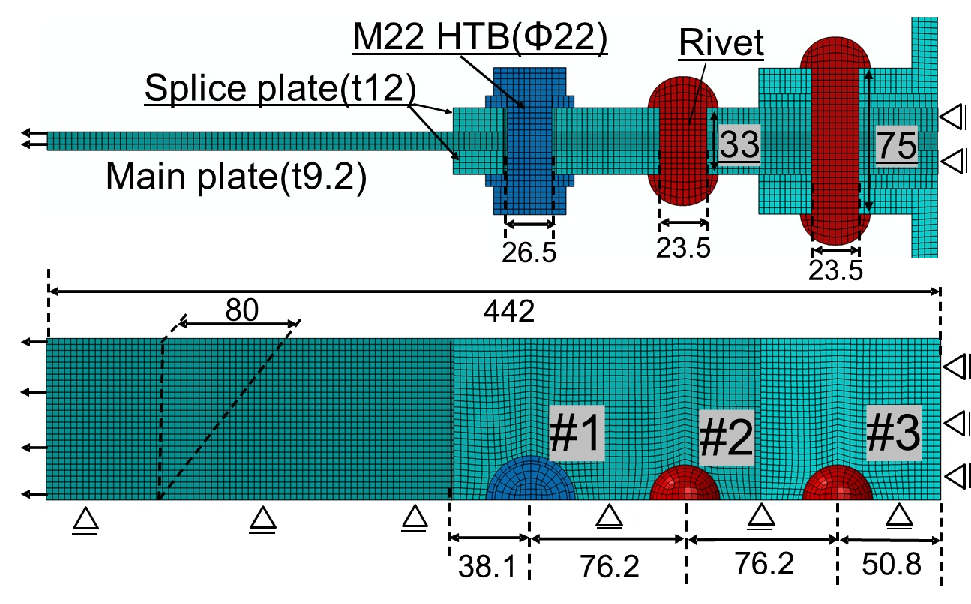
\includegraphics[width=0.75\linewidth]{imgs//ch4/femodel-hsbrive.pdf}
    \caption{FE Analysis model of hybrid joint combined with HSB and rivet (e.g. HSB1-b, Unit: mm)}
    \label{fig-femodel-hsbrive}
\end{figure}


% 
\begin{sidewaystable}[thp]
\caption{Analysis case and designed strength}
\label{tab-anacase-rivet}
\centering
\begin{tabular}{@{}lcccccccccccc@{}}
\toprule
\multirow{2}{*}{\begin{tabular}[c]{@{}c@{}}Case\\ Name\end{tabular}} & \multirow{2}{*}{\begin{tabular}[c]{@{}c@{}}Number \\ of Bolt\\ $n_{hsb}$\end{tabular}} & \multirow{2}{*}{\begin{tabular}[c]{@{}c@{}}Number\\ of Rivet\\ $n_{r}$\end{tabular}} & \multirow{2}{*}{\begin{tabular}[c]{@{}c@{}}Width\\ $b$\\ {[}mm{]}\end{tabular}} & \multicolumn{2}{c}{\begin{tabular}[c]{@{}c@{}}Designed \\ preload of Rivet\\ $N_r$ $[kN]$\\ Length of rivet shank\end{tabular}} & \begin{tabular}[c]{@{}c@{}}Designed \\ preload of\\ Bolt\\ $N_{hsb}$\end{tabular} & \begin{tabular}[c]{@{}c@{}}Slip \\ resistance\\ $F_{slip}$\end{tabular} & \begin{tabular}[c]{@{}c@{}}Net \\ Cross-section\\ yiled resistance\\ $F_{yp}$\end{tabular} & \begin{tabular}[c]{@{}c@{}}Modified \\ bearing\\ resistance\\ $F_{bp}$\end{tabular} & \multirow{2}{*}{\begin{tabular}[c]{@{}c@{}}$F_{yp}/F_{bp}$\\ $\gamma$\end{tabular}} & \multirow{2}{*}{\begin{tabular}[c]{@{}c@{}}$F_{yp}/F_{slip}$\\ $\beta$\end{tabular}} & \multirow{2}{*}{\begin{tabular}[c]{@{}c@{}}Expected \\ Serviceability \\ Limit State\end{tabular}} \\ \cmidrule(lr){5-6}
 &  &  &  & $33mm$ & $75mm$ & $[kN]$ & $[kN]$ & $[kN]$ & $[kN]$ &  &  &  \\ \midrule
HSB0-y & 0 & 3 & \multirow{8}{*}{102} & \multirow{7}{*}{45} & \multirow{7}{*}{78.5} & - & 70.8 & 199.2 & 249.6 & 0.80 & 2.81 & \multirow{8}{*}{\begin{tabular}[c]{@{}c@{}}Net \\ Cross-section \\ yiled limit\end{tabular}} \\
HSB1-y & \multirow{3}{*}{1} & \multirow{3}{*}{2} &  &  &  & \multirow{7}{*}{205} & 138.0 & 191.6 & \multirow{2}{*}{257.2} & 0.74 & 1.39 &  \\
HSB2-y &  &  &  &  &  &  & 138.0 & 199.2 &  & 0.77 & 1.44 &  \\
HSB3-y &  &  &  &  &  &  & 123.9 & 199.2 & 243.2 & 0.82 & 1.61 &  \\
HSB12-y & \multirow{3}{*}{2} & \multirow{3}{*}{1} &  &  &  &  & 205.2 & 191.6 & 264.7 & 0.72 & 0.93 &  \\
HSB13-y &  &  &  &  &  &  & 191.1 & 191.6 & \multirow{2}{*}{250.7} & 0.76 & 1.00 &  \\
HSB23-y &  &  &  &  &  &  & 191.1 & 199.2 &  & 0.79 & 1.04 &  \\
HSBall-y & 3 & 0 &  & \multicolumn{2}{c}{-} &  & 258.3 & 191.6 & - & - & - &  \\ \midrule
HSB0-b & 0 & 3 & \multirow{6}{*}{160} & \multirow{5}{*}{45} & \multirow{5}{*}{78.5} & - & 70.8 & 346.3 & 249.6 & 1.39 & 4.89 & \multirow{5}{*}{\begin{tabular}[c]{@{}c@{}}bearing \\ deformation\\ limit\end{tabular}} \\
HSB1-b & \multirow{3}{*}{1} & \multirow{3}{*}{2} &  &  &  & \multirow{5}{*}{205} & 138.0 & 338.7 & \multirow{2}{*}{257.2} & 1.32 & 2.46 &  \\
HSB2-b &  &  &  &  &  &  & 138.0 & 346.3 &  & 1.35 & 2.51 &  \\
HSB3-b &  &  &  &  &  &  & 123.9 & 346.3 & 243.2 & 1.42 & 2.80 &  \\
HSB23-b & 2 & 1 &  &  &  &  & 191.1 & 346.3 & 250.7 & 1.38 & 1.81 &  \\
HSBall-b & 3 & 0 &  & \multicolumn{2}{c}{-} &  & 258.3 & 338.7 & - & - & - & Slip limit \\ \bottomrule
\end{tabular}
\end{sidewaystable}


The boundary nonlinearity was modeled using the penalty method for contact and Coulomb friction for friction. In the literature \cite{rtri1992Manual}, it is reported that a slip coefficient of 0.25 to 0.28 can be expected when rivets are replaced with high-strength bolts while leaving leadite on the joint surface. On the other hand, in a separate test conducted by the authors to confirm the coefficient of slip of joint surfaces with lead-pan coating, the coefficient of slip at girder joints ranged from 0.15 to 0.38 \cite{Chen2021}. Based on the above, a coefficient of friction of 0.21 was given as the coefficient of friction for the case with lead-pan coating in this analysis, referring to the average value of the coefficient of slip in the literature.

In this study, a total of 14 analytical cases shown in Table \ref{tab-anacase-rivet} were set up using the rivet and high-strength bolt arrangements and the plate width b of the material to be joined as parameters. The cross-sectional shapes of the analysis cases do not change the bearing capacity of the main plate, so the plate thickness and material are not changed, and only the plate width is changed.

For the names of the analysis cases, HSB represents a high-strength bolt, the number following it indicates the location of the high-strength bolt, and y: yield-precedence type and b: bearing pressure-precedence type indicate the expected service limit mode. In this study, rivets and high-strength bolts are collectively referred to as fasteners.

Fasteners were positioned from the outside of the joint to the inside as shown in Figure 2, from 1 to 3.

For example, HSB1-y means a case with one high-strength bolt at fastener position 1 and a rivet in combination with a yield-precedence type. HSBall is a case where all fastener positions 1, 2, and 3 are high-strength bolts.

The stress-strain relationships of the materials used in the analysis are shown in Fig. \ref{fig-anarivet-mt} and the mechanical properties in Table \ref{tab-anarivet-mt}. The constitutive law of each material was modeled as a bilinear type with a quadratic stiffness of $E/100 (E=200,000 MPa)$, and the mechanical properties of the main plate and the riveted plate were obtained from material test results cut from the transverse girder of the A Bridge. For the mechanical properties of the rivets, the results of tensile tests \cite{KOMATSU2015} on the rivets of the Hokko Bridge (completed in 1932), which uses the same type of rivets as those of the A Bridge, were used.


\begin{table}
    \centering
    \caption{Mechanical properties of materials}
    \label{tab-anarivet-mt}
    \begin{tabular}{cccc}
    \toprule
        \multirow{2}{*}{\begin{tabular}[c]{@{}c@{}} Member\end{tabular}}  &
        \multirow{2}{*}{\begin{tabular}[c]{@{}c@{}} Class\end{tabular}} & 
        Yiled Strength & Ultimate Strength\\ 
         &  & $N/mm^2$ & $N/mm^2$ \\ \midrule
        Steel plate & St39 & 275.8 & 454 \\
        Rivet & SV34 & 295 & 389 \\
        HTB	& F10T & 900 & 1000 \\
    \bottomrule
    \end{tabular}
\end{table}

\begin{figure}[htbp]
    \centering
    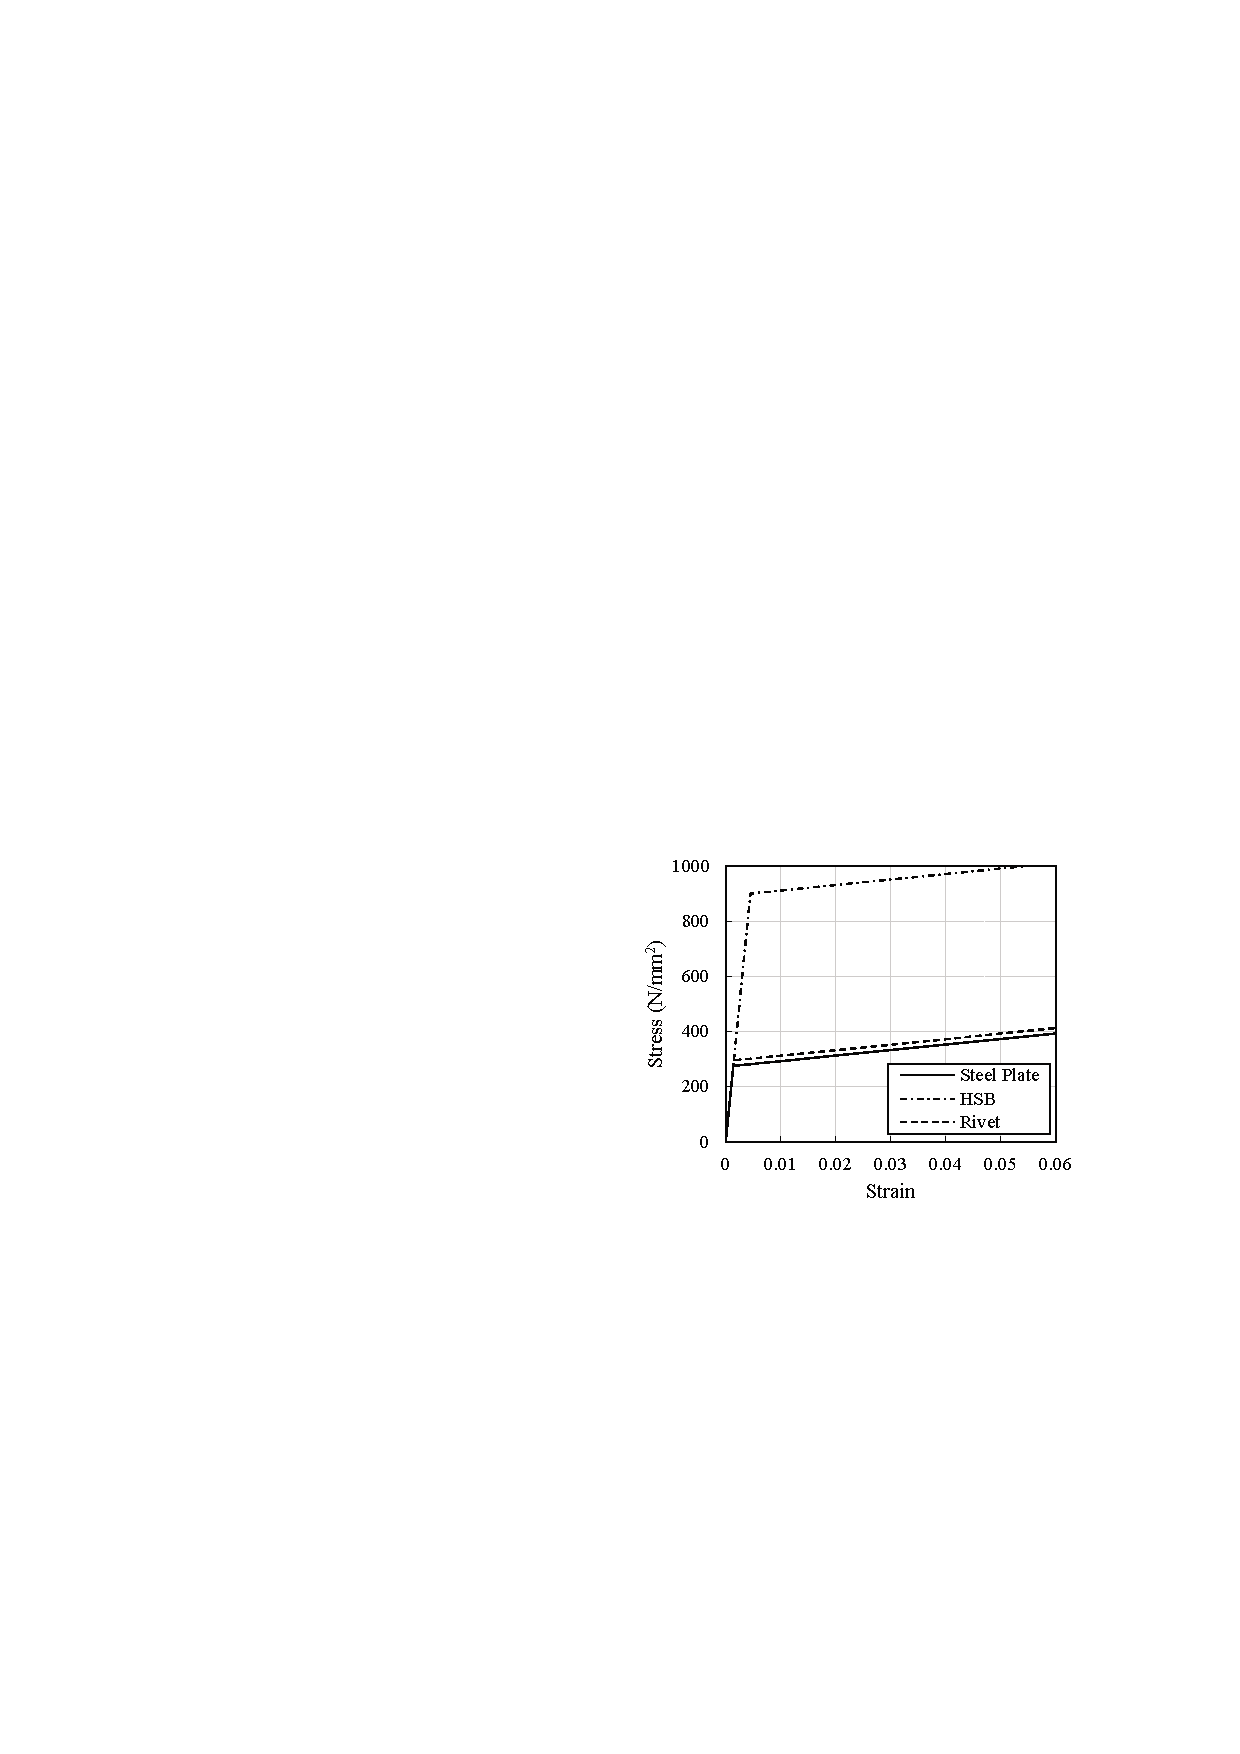
\includegraphics[width=0.55\linewidth]{imgs//ch4/rivet-mt-ch3.pdf}
    \caption{Stress-strain relationship used in the analysis}
    \label{fig-anarivet-mt}
\end{figure}

In the analysis, initial preloads were introduced to the rivets and high-strength bolts in Step 1, and tensile forces due to forced displacement were applied to the end of the material to be joined in Step 2.

The bolt and rivet preloads were introduced in the analysis by setting up a reference section in the center of the rivet and high-strength bolt shafts and applying initial bolt preloads to the reference section using the bolt loading option in Abaqus / Standard. In subsequent loading steps, the reference section displacement changed by the introduction of the bolt preload is fixed so that changes in the bolt preload can be taken into account. The Poisson's ratio $v$ of the rivet is set to 0 because the rivet's axial diameter is reduced by the Poisson's effect when the preload is introduced and the initial state of support between the rivet and rivet hole cannot be reproduced.

For the rivet preload $N_r$ , the literature \cite{Heinemeyer2011TheConnections} reported that the rivet preload depends on the shaft length and that for rivets with a diameter of 22 mm, the rivet preload/rivet shaft yield strength ratio for a shaft length of 33 mm was 0.4 on average and the rivet preload/rivet shaft yield strength ratio for a shaft length of 75 mm was 0.7 on average. The rivet shaft force/rivet shaft yield strength ratio used in Bridge A was reported to be 0.7 on average. The average yield strength of the rivets used in Bridge A is assumed to be 295 MPa \cite{KOMATSU2015}, so rivet shaft forces of 45 $kN$ for a shaft length of 33 mm and 78.5 $kN$ for a shaft length of 75 mm were introduced.
 
\subsubsection{Bearing resistance per Fastener}\label{ch4sec2-1}

The bearing capacity, shear capacity and slip capacity per fastener are shown in Table \ref{ch4tab3}.

\begin{table}[]
\caption{Resistance per fastener}
\label{ch4tab3}
\centering
\begin{tabular}{@{}lcccccc@{}}
\toprule
\multicolumn{2}{c}{\multirow{3}{*}{Fastener}} & \multirow{2}{*}{\begin{tabular}[c]{@{}c@{}}Friction\\ Coefficient\end{tabular}} & Preload & \multicolumn{3}{c}{Resistance per fastener} \\ \cmidrule(l){5-7} 
\multicolumn{2}{c}{} &  & $N_f$ & Slip & Bearing & Shear \\
\multicolumn{2}{c}{} & $\mu$ & $[kN]$ & $F_{s1}$ & $F_{bs1}$ & $F_{sh1}$ \\ \midrule
\multirow{2}{*}{Rivet} & 33mm & \multirow{3}{*}{0.21} & 45 & 18.9 & \multirow{2}{*}{89.4} & \multirow{2}{*}{127.3} \\
 & 75mm &  & 78.5 & 32.97 &  &  \\
\multicolumn{2}{c}{HSB} &  & 205 & 86.1 & 83.7 & 395.0 \\ \bottomrule
\end{tabular}
\end{table}


In the area subjected to bearing, plastic flow is unlikely to occur due to the surrounding restraints, and strength above the yield strength can be expected. For this reason, the bearing strength $\sigma_{bs}$ should be 1.5 times the yield strength of the main plate $\sigma_{yp}$ as shown in Equation \ref{eq-sigbs}. In this study, the bearing resistance per rivet $F_bjr1$ was calculated from the railroad standard equation \ref{eq-fbs}. The shear strength of the rivets is given by Equation \ref{eq-tauyf}, and the shear yield capacity per rivet, $F_v1$, is calculated from Equation \ref{eq-fsh1}. The slip resistance per fastener $F_{s1}$ is given by Equation \ref{eq-fs1}.

\begin{equation}\label{eq-sigbs}
    \sigma_{bs}=1.5\sigma_{yp}
\end{equation}
\begin{equation}\label{eq-fbs}
    F_{bjr1}=d_f t\sigma_{bs}
\end{equation}
\begin{equation}\label{eq-tauyf}
    \tau_{yf}=\sigma_{yf}/\sqrt{3}
\end{equation}
\begin{equation}\label{eq-fsh1}
    F_{v1}=\pi (0.5d_f)^2 \tau_{yf} m
\end{equation}
\begin{equation}\label{eq-fs1}
    F_{s1}=\mu m N_f
\end{equation}

where, $\sigma_{bs}$: bearing strength, $\sigma_{yp}$ : yield strength of the main plate, $t$: thickness of the main plate, $d_f$ : diameter of fastener, $F_{bs1}$: bearing resistance of one fastener, $\sigma_{yf}$ : yield strength of the fastener, $\tau_{yf}$ : shear strength of fastener, $F_{sh1}$ : shear resistance of one fastener, $F_{s1}$ : slip resistance of one fastener, $m$ : the number of shear plane, $N_f$ : perload of fastener.


\subsubsection{Design Strength of Joints}

In this study, the design bearing capacity for the service limit was obtained as follows

The slip resistance $F_{slip}$ and the net cross-section yield resistance 
$F_{yp}$ of the joint is calculated from the total value of each fastener in Eq. \ref{fslip-ch4} and Eq. \ref{fyp-ch4} respectively.

\begin{equation}\label{fslip-ch4}
    F_{slip} = \sum F_{s1}
\end{equation}
\begin{equation}\label{fyp-ch4}
    F_{yp} = (w-d_1)t\times \sigma_{yp}
\end{equation}

where, $F_{slip}$ : slip resistance of the joint, $w$ : width of the main plate, $d1$ : diameter of the hole at outermost fastener.

It is assumed that after the main slip occurs, the frictional resistance force is not taken into account and the load is entirely carried by the bearing resistance in a friction joint \cite{rivet1977}. However, in actual behavior, the frictional resistance force remains to some extent even after slip occurs. On the other hand, the road map and railroad standards do not clearly indicate the limit state of bearing capacity in riveted joints.

In the literature \cite{hashimoto2008}, the bearing capacity of a combined joint using rivets and high-strength bolts was proposed as shown in Equation (8). However, this equation does not take into account the design bearing capacity at the service limit and the rivet preload that affects the load transfer condition. On the other hand, the bearing capacity of the rivet in Equation (8) uses the yield strength of the rivet and focuses on the yield of the rivet shaft, which may not be appropriate when the material to be joined is a thin plate or when the yield strength of the material to be joined is lower than the rivet.

Therefore, this study proposes an improved bearing capacity as the design bearing capacity of a combined joint that considers the preload of the rivet and focuses on the yield of the rivet hole in the material to be jointed.,$F_{bm}$. The improved bearing capacity is proposed as the design bearing capacity of the joints with rivet holes. The improved bearing capacity,F-bp. is calculated as the sum of the slip capacity and bearing capacity of each fastener using Equation (9). Here, the bearing capacity per rivet is not the standard bearing capacity of the railroad, but the yield strength of the material to be jointed.1.5,σ-y. but from the yield strength of the material to be jointed.1.0,σ-y. The bearing capacity per rivet is calculated based on the yield strength of the material to be joined, rather than the standard bearing strength of the railway. The effective area of bearing capacity assumes that the shaft of the rivet is in contact with the hole and that load is transmitted in the projected area of the rivet shaft.

\begin{equation}\label{eq-fbhashi}
    F_{b,hashimoto}=n_b μmN_b + n_r \times 1.5d_r tσ_yr
\end{equation}
\begin{equation}
    F_{bp,rivet}=μm(n_b N_b+n_r N_r)+n_r d_r tσ_y
\end{equation}

where,$F_b.$ : bearing capacity by Hashimoto et al.,$F_bp$. : the improved bearing capacity proposed in this study, $n_b$: Number of high-strength bolts, $n_r$ Number of rivets, $N_b$: preload of high strength bolts. $N_r$ : preload of rivets. $\sigma_{yr}$ : Yield strength of rivet, $σ_y$ : Yield strength of the main plate, $t$ : thickness of the material to be joined, $d_r$: rivet shaft diameter.

\subsection{Results and Discussions}

\subsubsection{Limit states of use of joints in combination}

In this study, we focused on the overall displacement of the joint and plasticization around the hole, and defined the service limit state of the joint as the time when the load-overall displacement relationship of the joint begins to exhibit nonlinear behavior. The nonlinear behavior of the joint is governed by the yielding of the rivet hole or the pure section.

In this analysis, the bearing load $P_{bya}$ is defined as the load at which all the rivet holes in the main plate yield. Yield of a rivet hole is defined as the time when equivalent plastic strain occurs at all six integration points of the rivet hole wall, as shown in Fig. \ref{fig-posieqqe}. The net cross-sectional yield load is defined as the equivalent plastic strain at the net cross-sectional location of the kovar surface.

\begin{figure}[htbp]
    \centering
    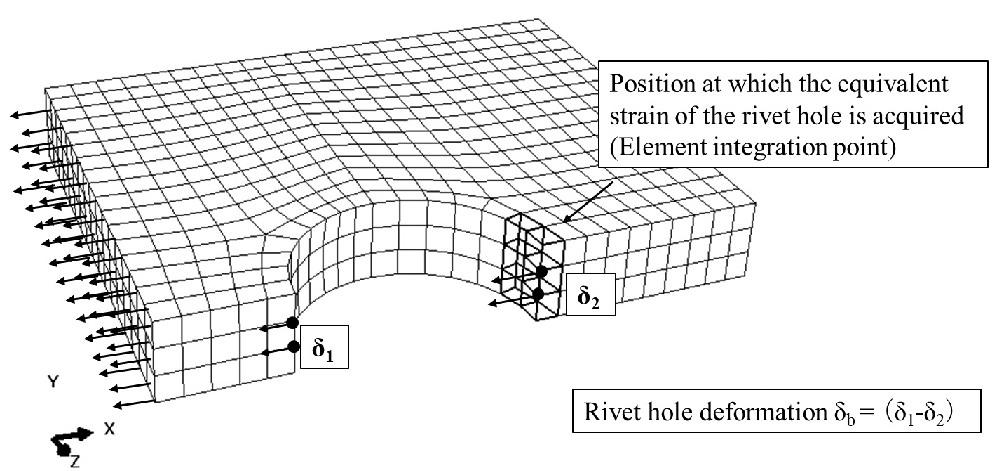
\includegraphics[width=0.75\linewidth]{imgs//ch4/posi-eqqe.pdf}
    \caption{Equivalent strain and the rivet hole deformation}
    \label{fig-posieqqe}
\end{figure}

Fig. \ref{fig-ls-ch4} shows the relationship between load and equivalent plastic strain of the fastener hole in the riveted HSB0-b joint, and Fig. \ref{fig-ld-htb0b} shows the relationship between load and overall displacement of HSB0-b. As shown in Fig. \ref{fig-femodel-hsbrive}, the overall displacement is the amount of forced displacement applied to the end of the joint.

\begin{figure}[htbp]
    \centering
    \begin{minipage}[t]{0.48\textwidth}
    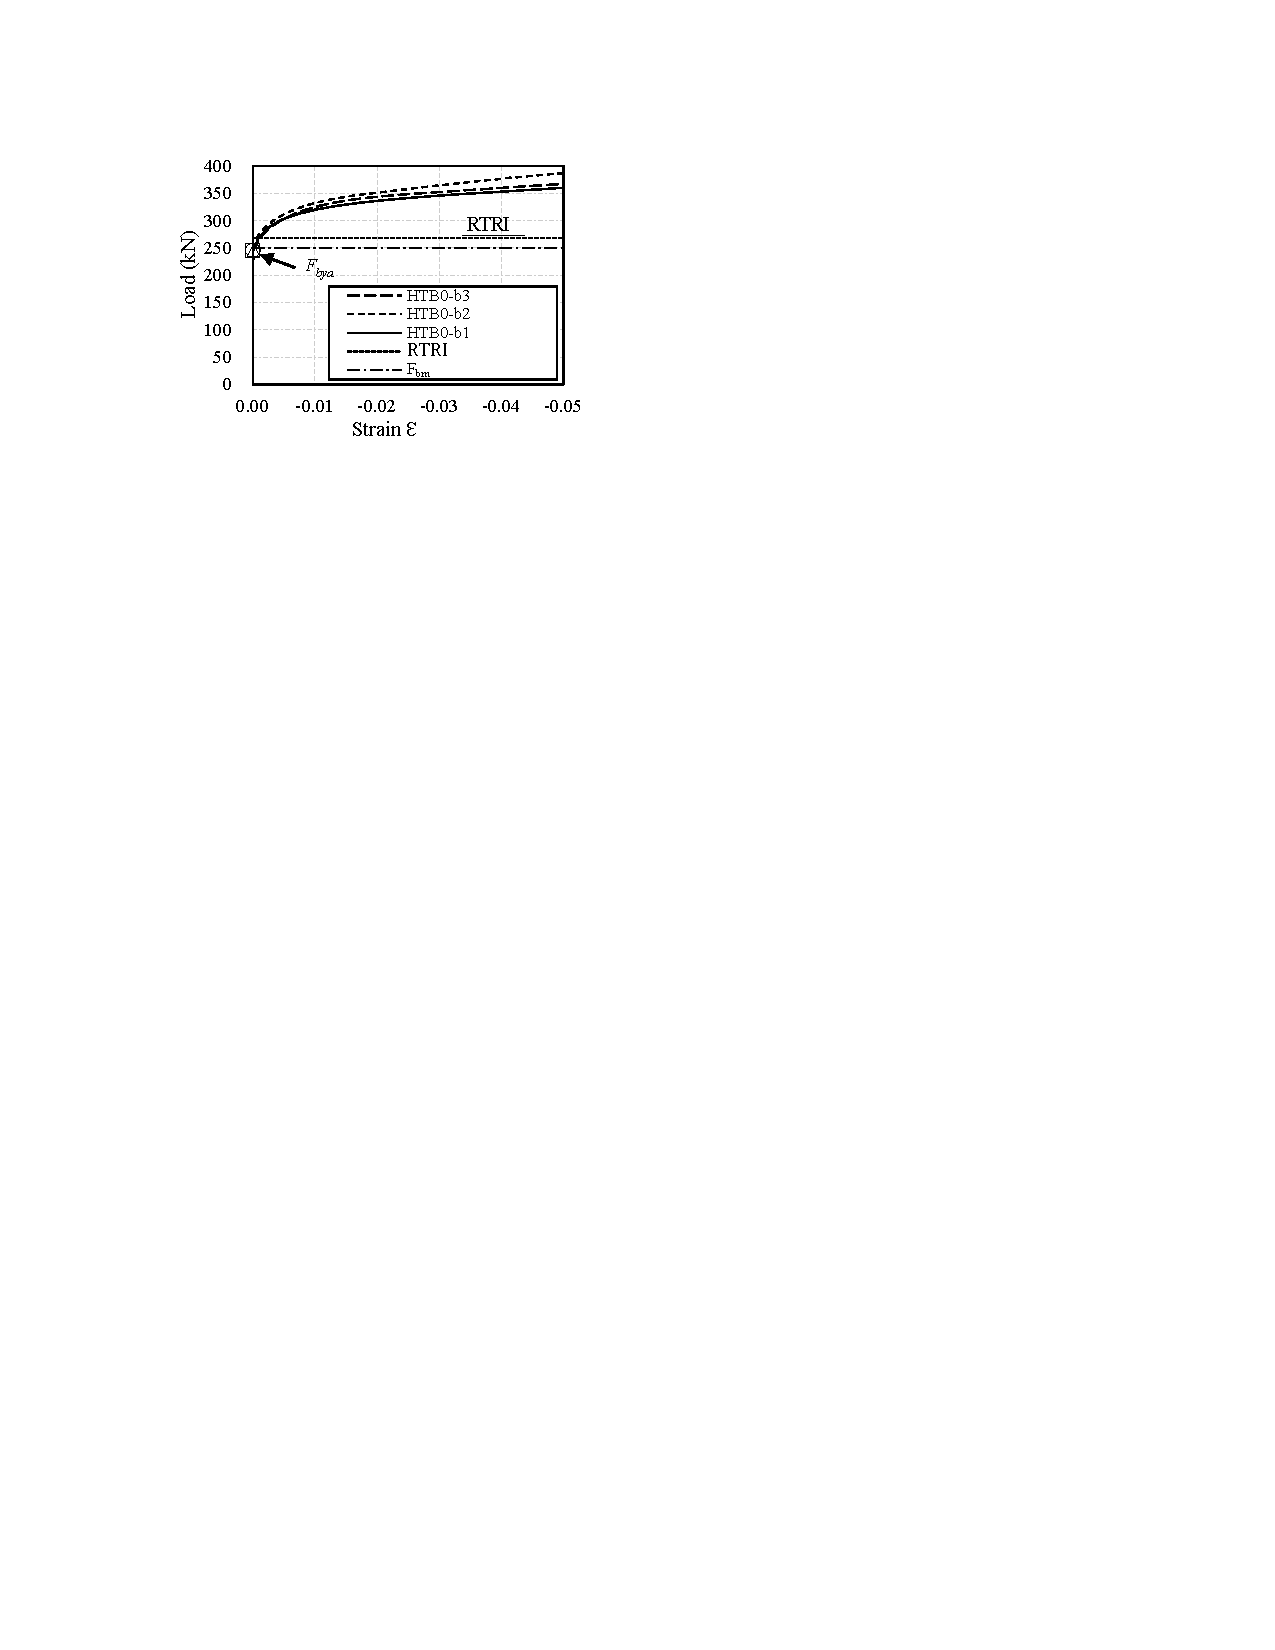
\includegraphics{imgs/ch4/LS-ch4.pdf}
    \caption{Relationship between load and strain}
    \label{fig-ls-ch4}
    \end{minipage}
    \begin{minipage}[t]{0.48\textwidth}
    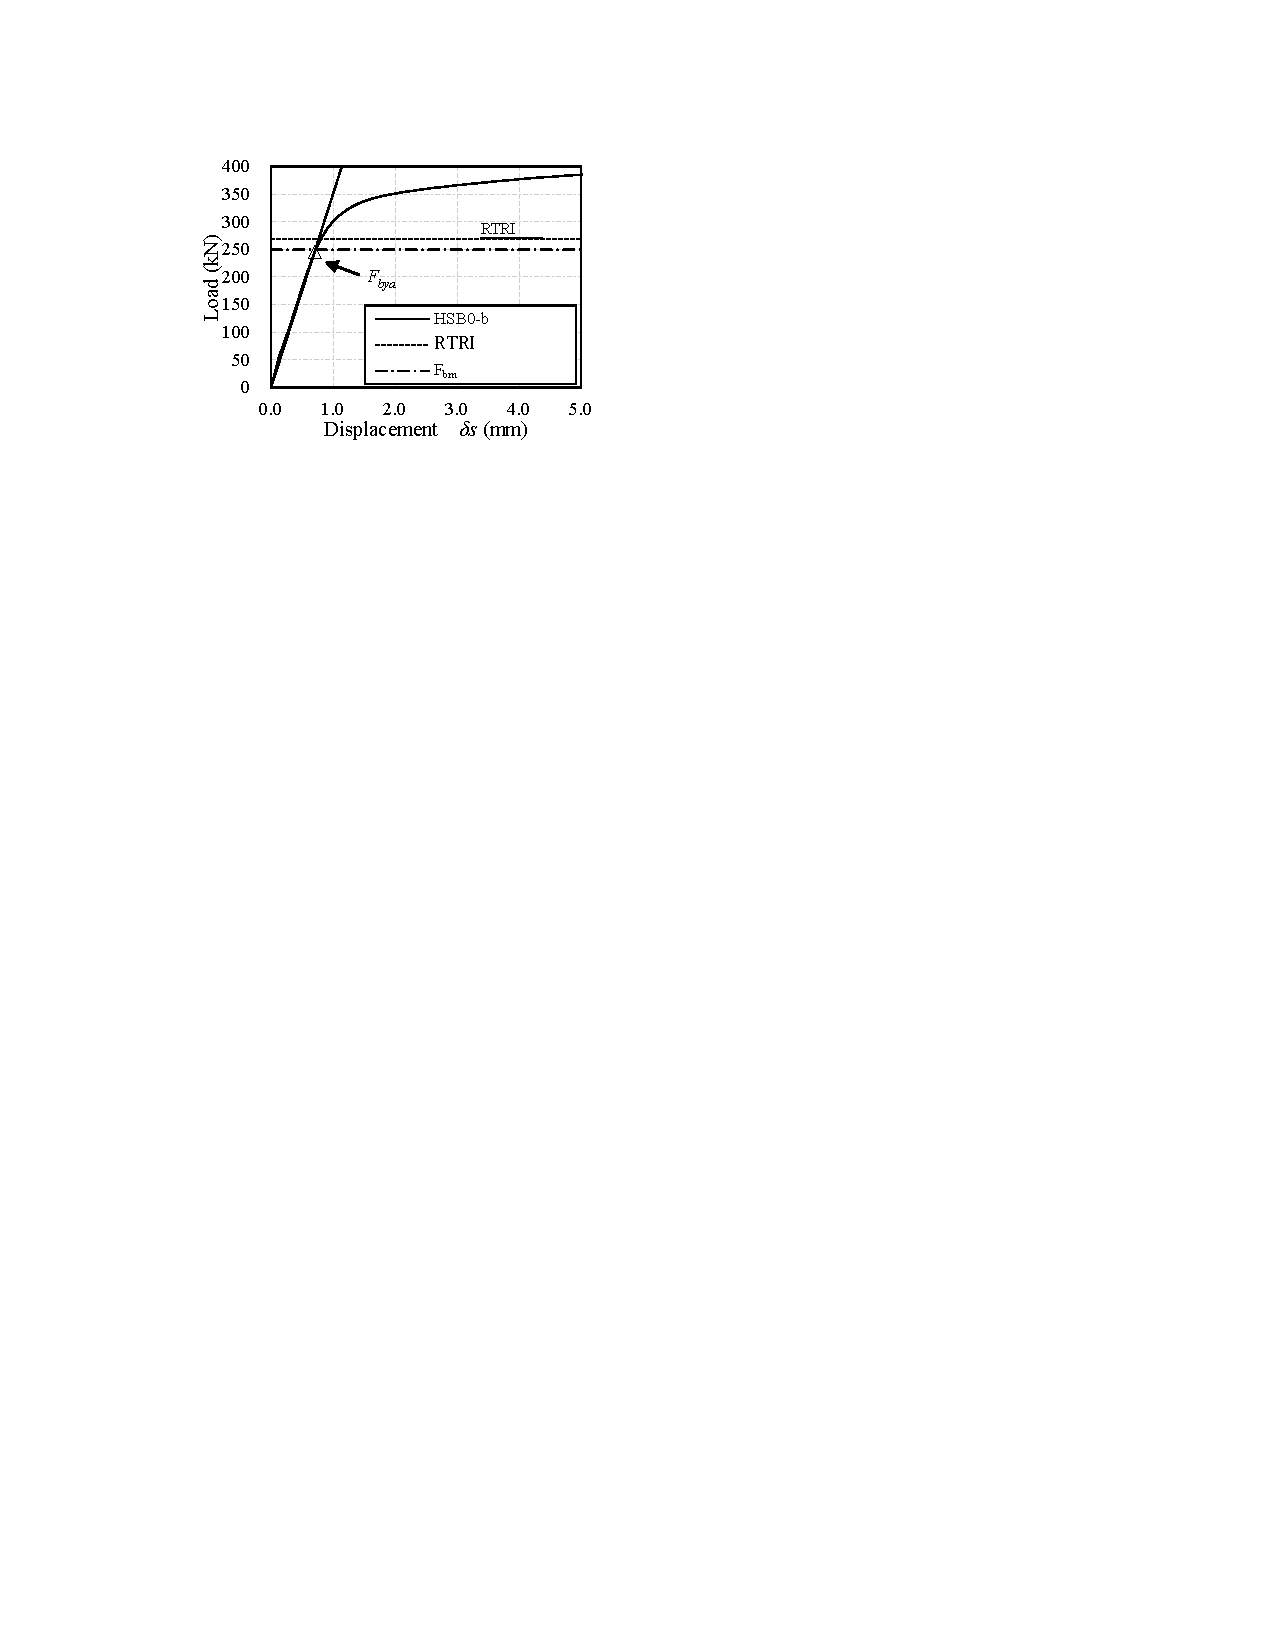
\includegraphics{imgs/ch4/ld-htb0b.pdf}
    \caption{Relationship between load and displacement (HTB0-b)}
    \label{fig-ld-htb0b}
    \end{minipage}
    \begin{minipage}[t]{0.48\textwidth}
    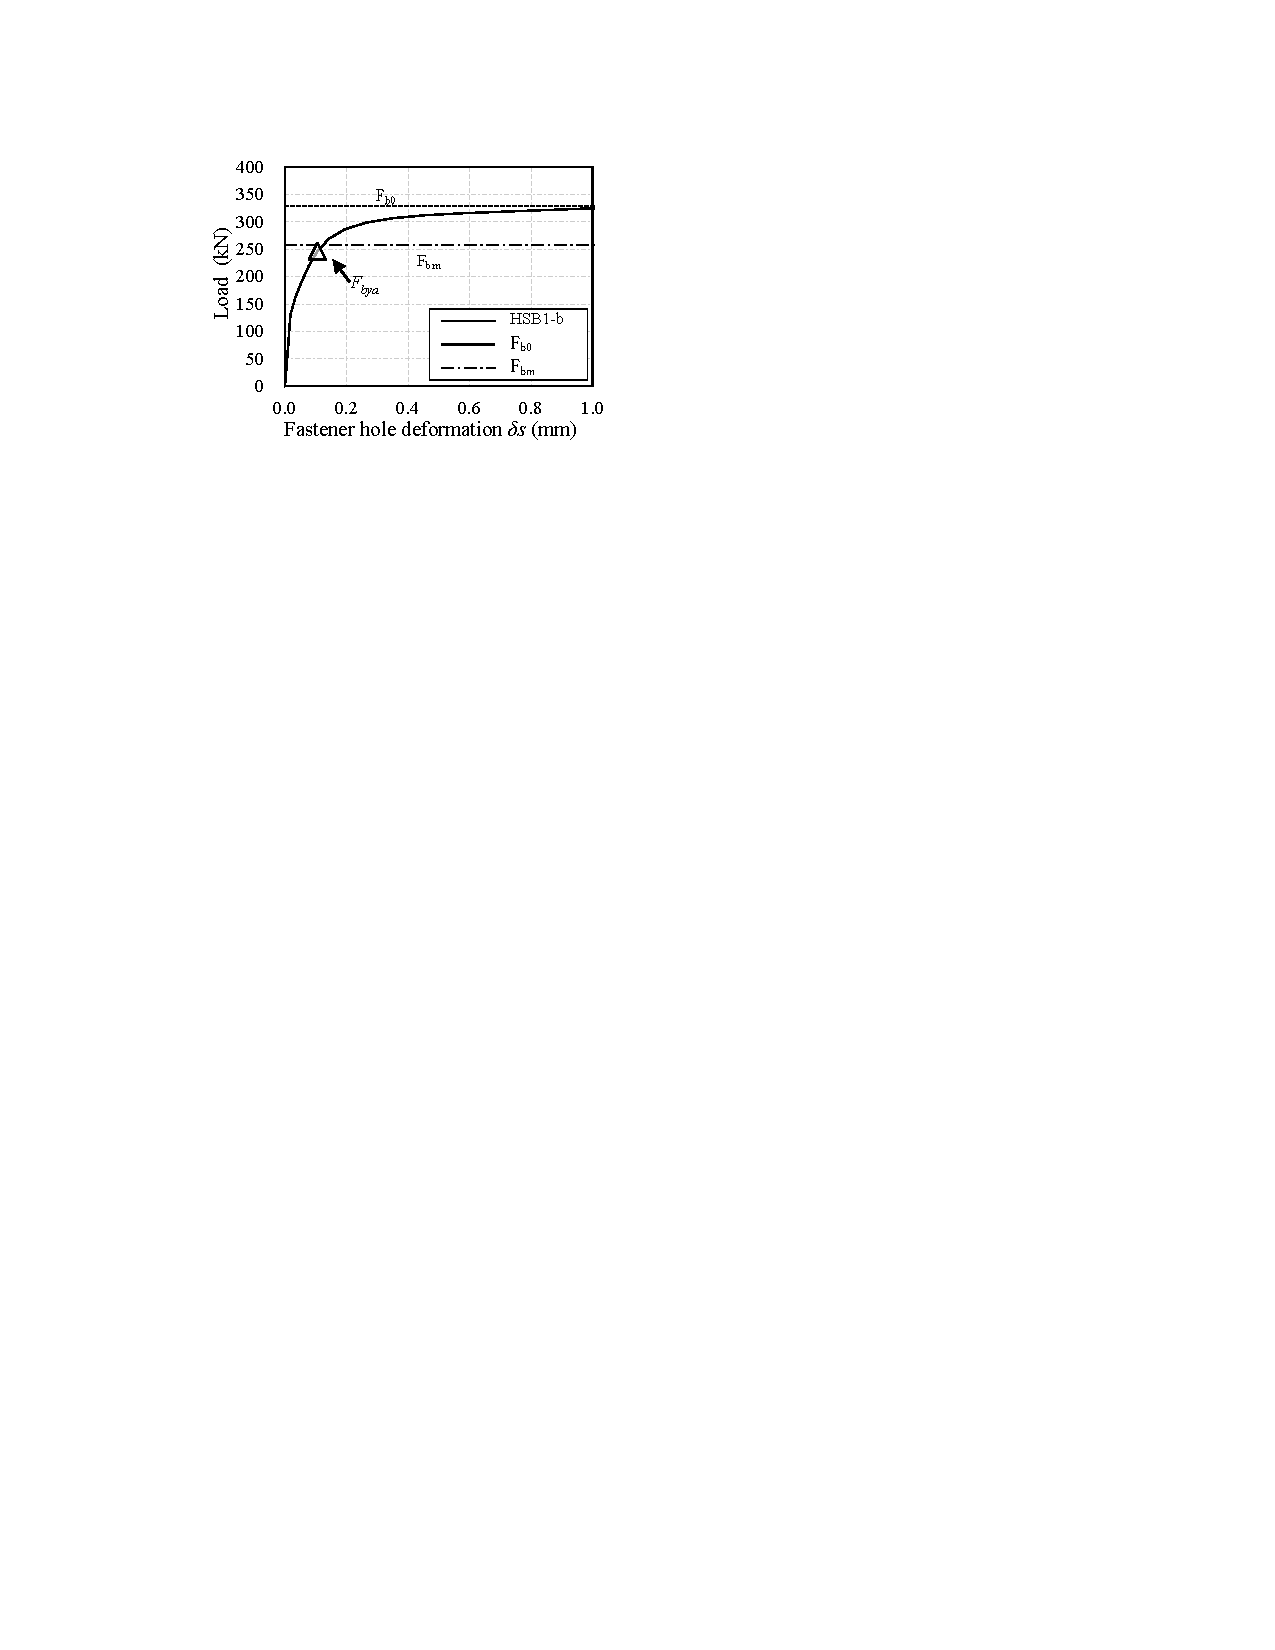
\includegraphics{imgs/ch4/lfhd-ch4.pdf}
    \caption{Relationship between load and fastener hole deformation (HTB1-b)}
    \label{fig-lfhd-ch4}
    \end{minipage}
    \begin{minipage}[t]{0.48\textwidth}
    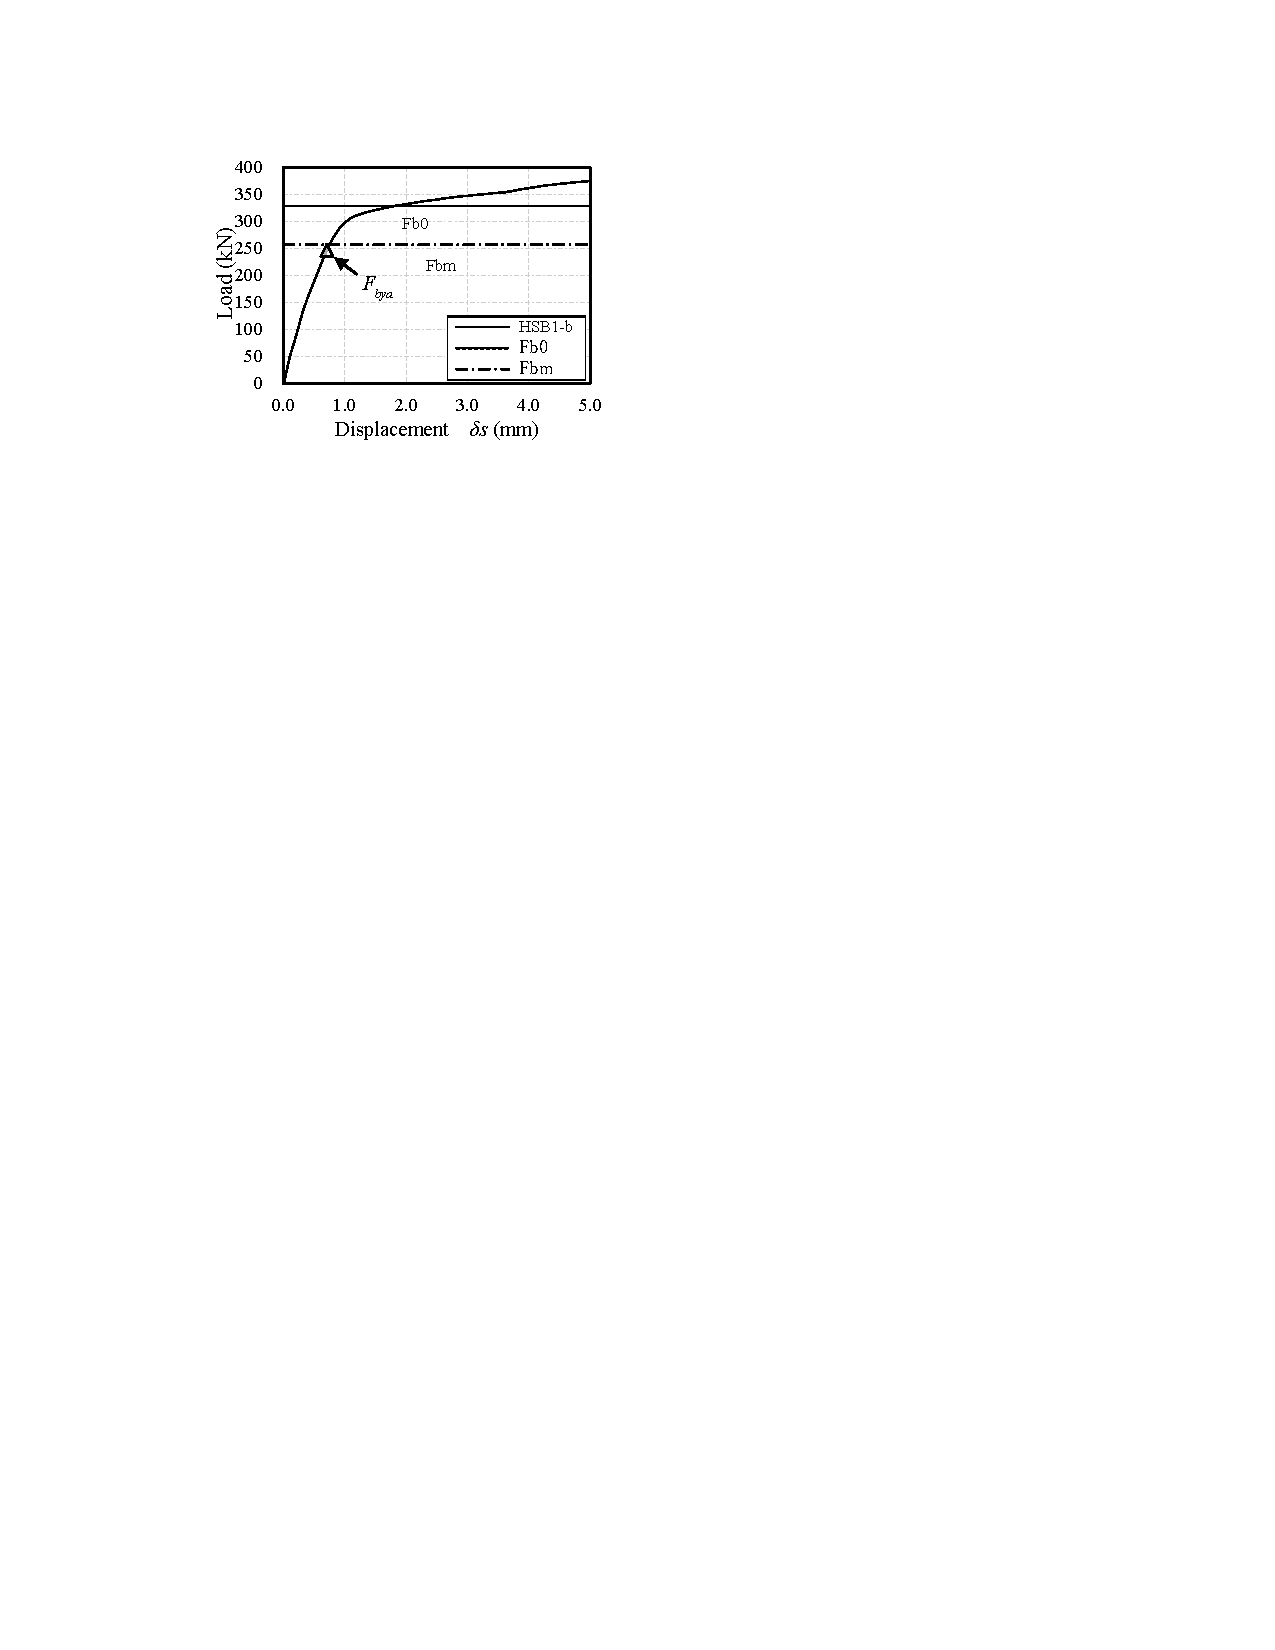
\includegraphics{imgs/ch4/ld-htb1b.pdf}
    \caption{Relationship between load and displacement (HTB1-b)}
    \label{fig-8ch4}
    \end{minipage}
    
\end{figure}

Fig.\ref{fig-lfhd-ch4} and Fig. \ref{fig-8ch4} show the load-displacement relationship for HSB1-b and the total deformation of the three fastener holes, respectively. Note that the bearing load $P_{bya}$ is plotted as △.

Figure 5 shows that the bearing capacity of HSB0-b ($P_{bya}$ = 245 $kN$) is comparable to the improved bearing capacity proposed in this study (Fbp = 249.6 $kN$). Figures 6, 7, and 8 show that the load-total displacement relationship for both the riveted and combined joints exhibited nonlinear behavior once the bearing capacity load $P_{bya}$ was reached.

\begin{figure}[htbp]
    \centering
    \begin{minipage}[t]{1\textwidth}
    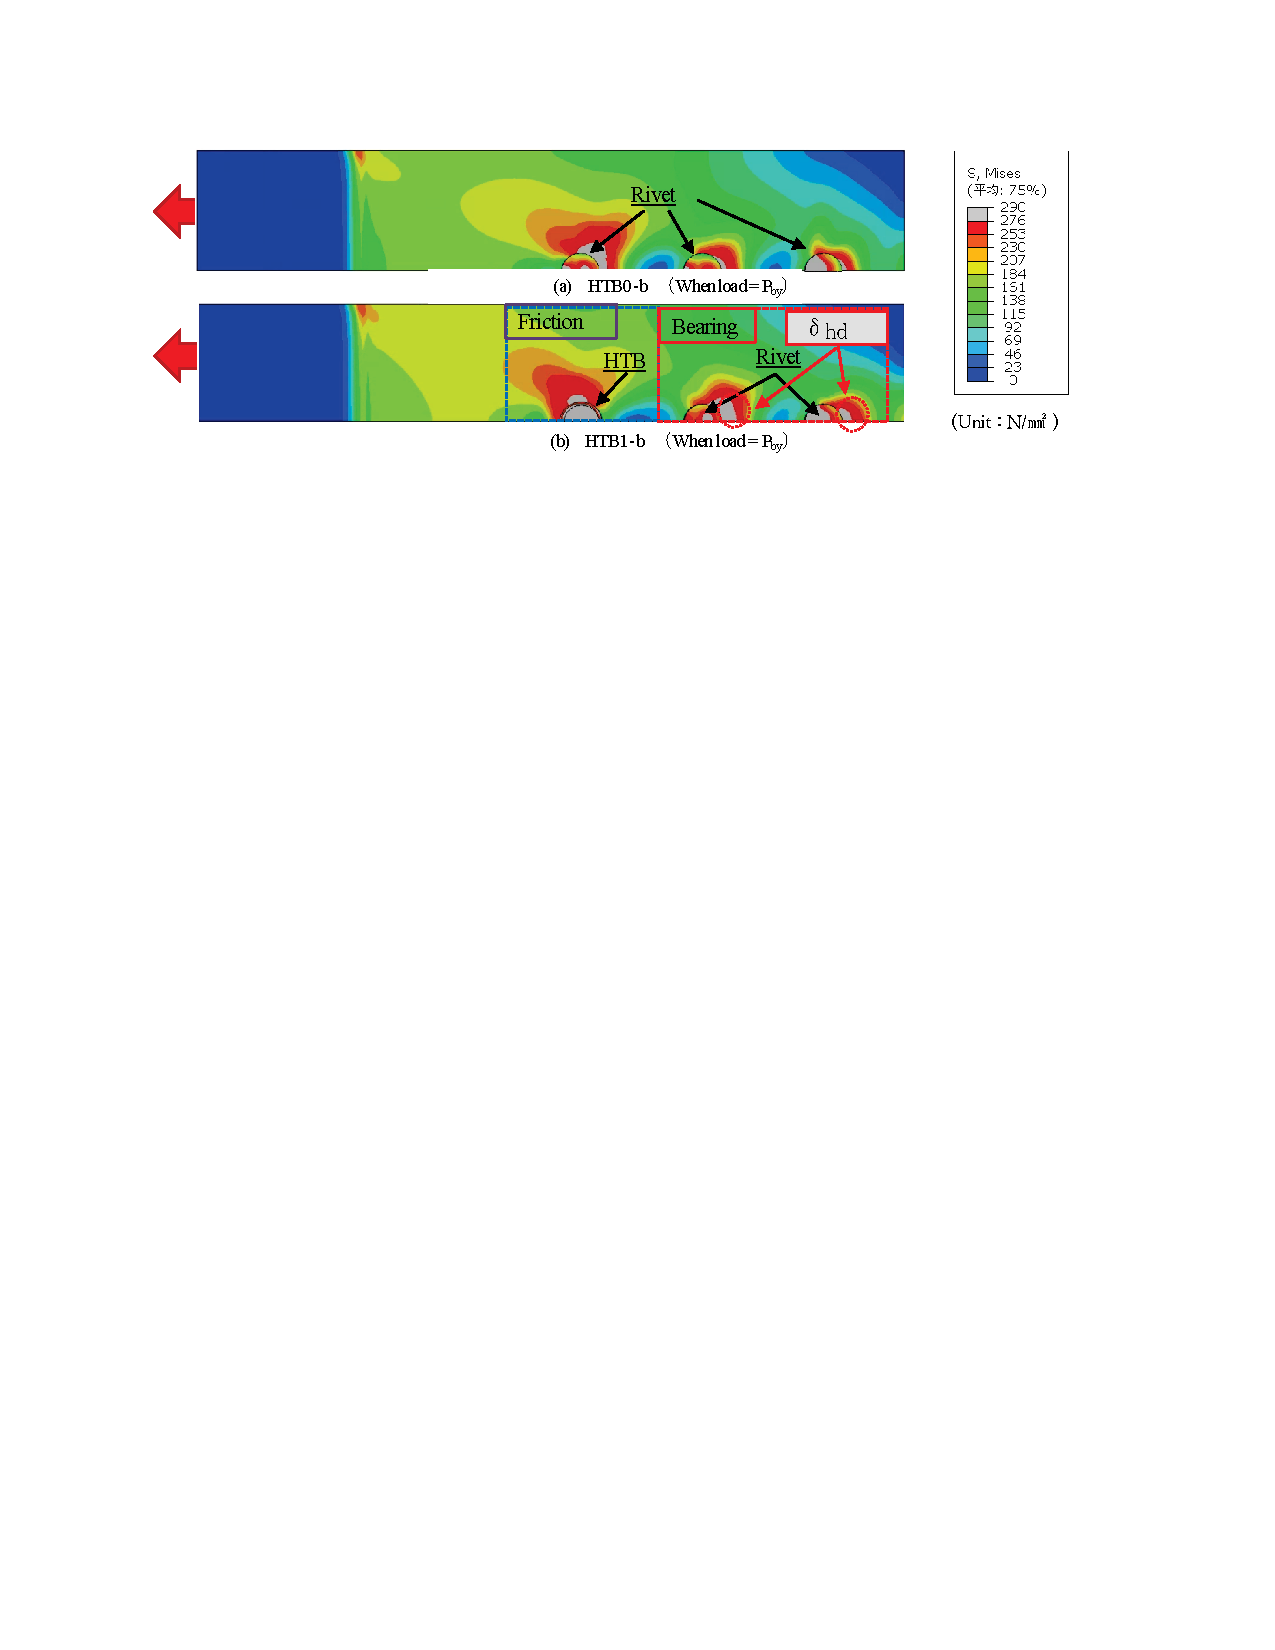
\includegraphics{imgs/ch4/ch4fig9.pdf}
    \caption{Mises stress counter of the joint (thickness center of main plate)}
    \label{fig-9-ch4}
    \end{minipage}
    \begin{minipage}[t]{1\textwidth}
    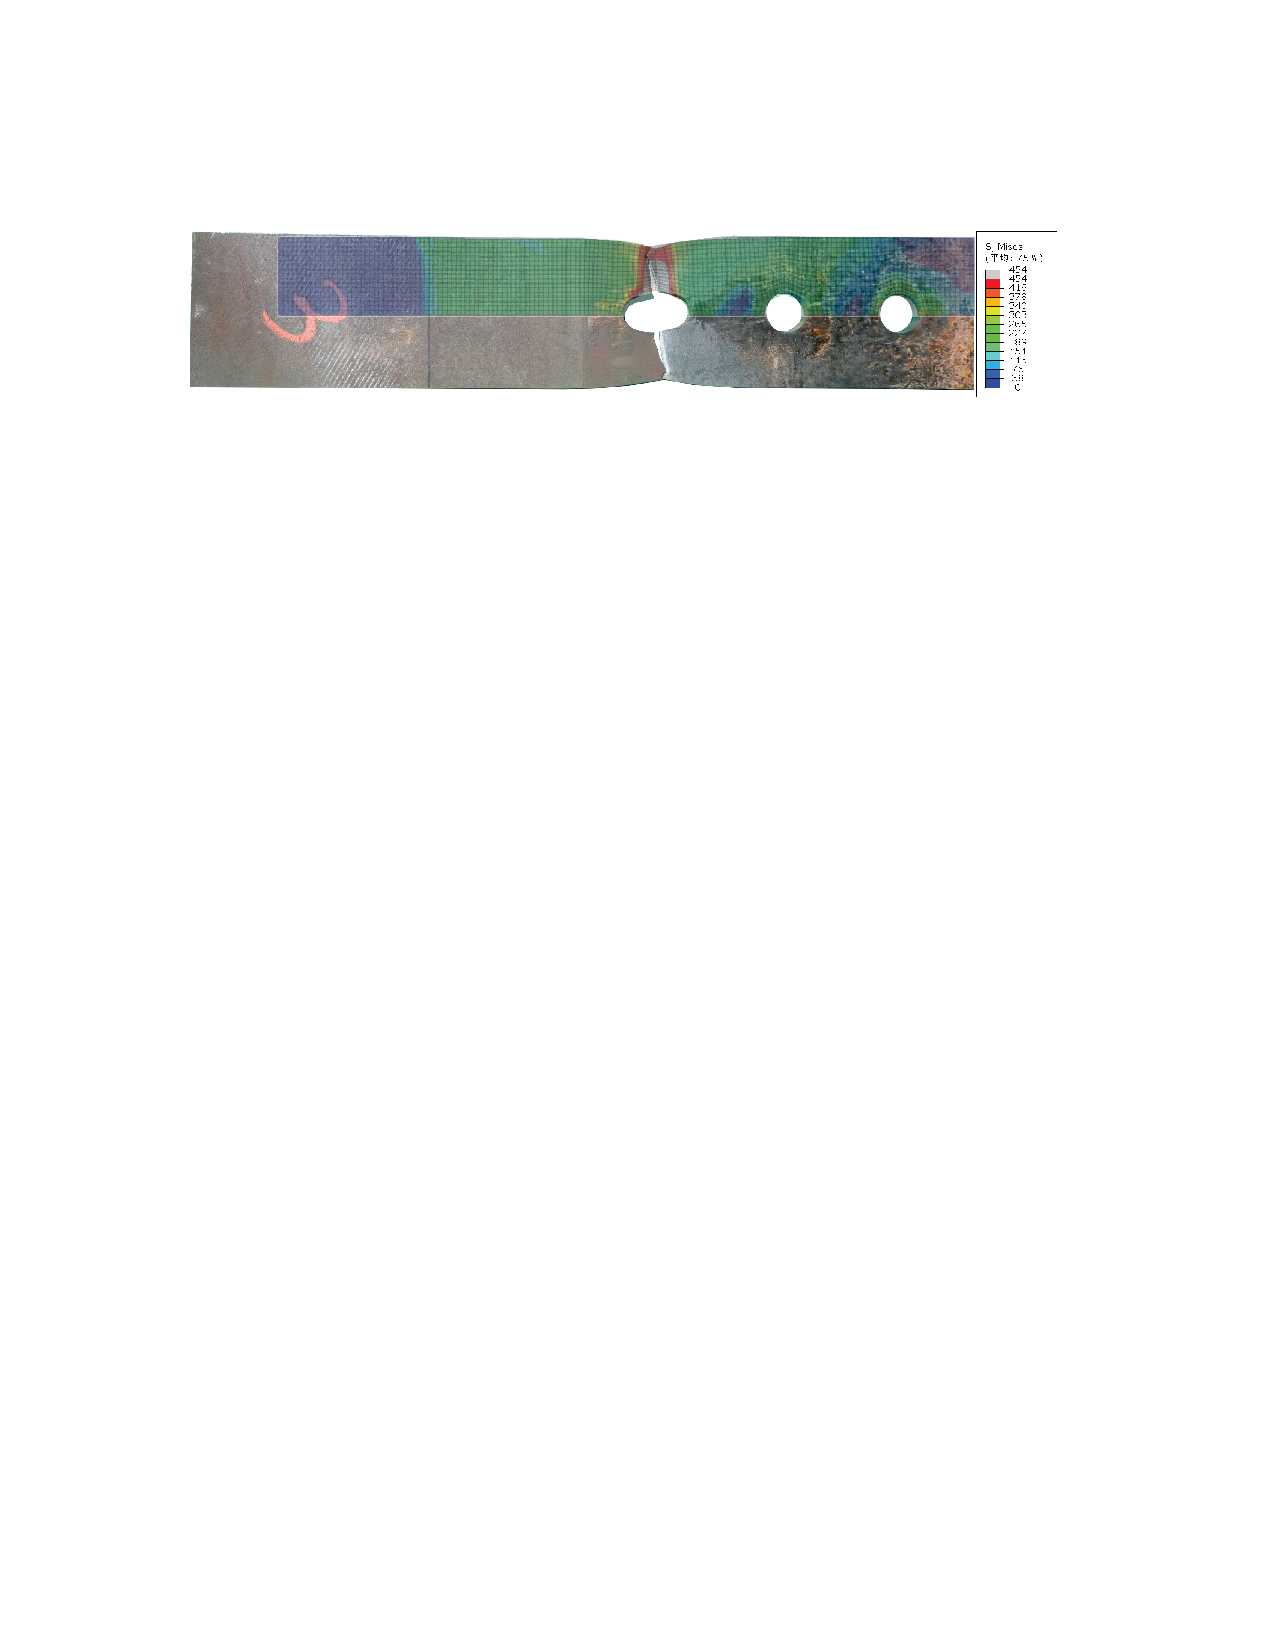
\includegraphics{imgs/ch4/ch4fig10.pdf}
    \caption{Relationship between load and displacement (HTB0-b)}
    \label{ch4fig10}
    \end{minipage}
\end{figure}


Fig. \ref{fig-9-ch4} shows the Mises stress contours at the center of the thickness of the material to be welded when HSB0-b and HSB1-b reach the bearing load $P_{bya}$ .

Fig. \ref{fig-9-ch4} shows that the degree of plasticization of the rivet holes is not uniform at a bearing load $P_{bya}$ , and is smallest at fastener position 3 and largest at fastener position 1. ybpThe γ in equation (10) is used to classify the service limit state of the combined joints as the pure sectional yield-precedence type when γ is greater than 1 and the pressure-precedence type when γ is less than 1. F  and F  were calculated from the pure sectional yield capacity equation (7) and the improved bearing capacity equation (9), respectively.
$γ=,F-y./,F-bp.$ (10)

γ<1 : net sectional yield first type


γ>1 : Bearing yield first type %支圧先行


\subsubsection{Mechanical behavior}

Fig. \ref{ch4fig10} shows the Mises stress contours and the fracture plan of the base material of the specimen under study at the maximum load of HSBall-y.

Fig. \ref{ch4fig10} shows that the deformation and failure location of the pure section obtained from the FEM analysis were almost consistent with the experimental results. The ultimate state is considered to be pure section rupture because the tensile strength of the entire pure section is reached in all cases of the analysis, as shown in Figure 10.


Figures 11.b and 12.b show the case with one high-strength bolt, while Figures 11.c and 12.c show the enlarged view near the net section yield load for the case with two high-strength bolts. Here, the obtained bearing load $P_{bya}$ is indicated by a large symbol. The slope between the load and the overall displacement of the joint is defined as the stiffness, and the initial stiffness change point is defined as the time when the entire joint begins to exhibit nonlinear behavior.

\begin{figure}[htbp]
    \centering
    \begin{subfigure}[t]{0.75\textwidth}
    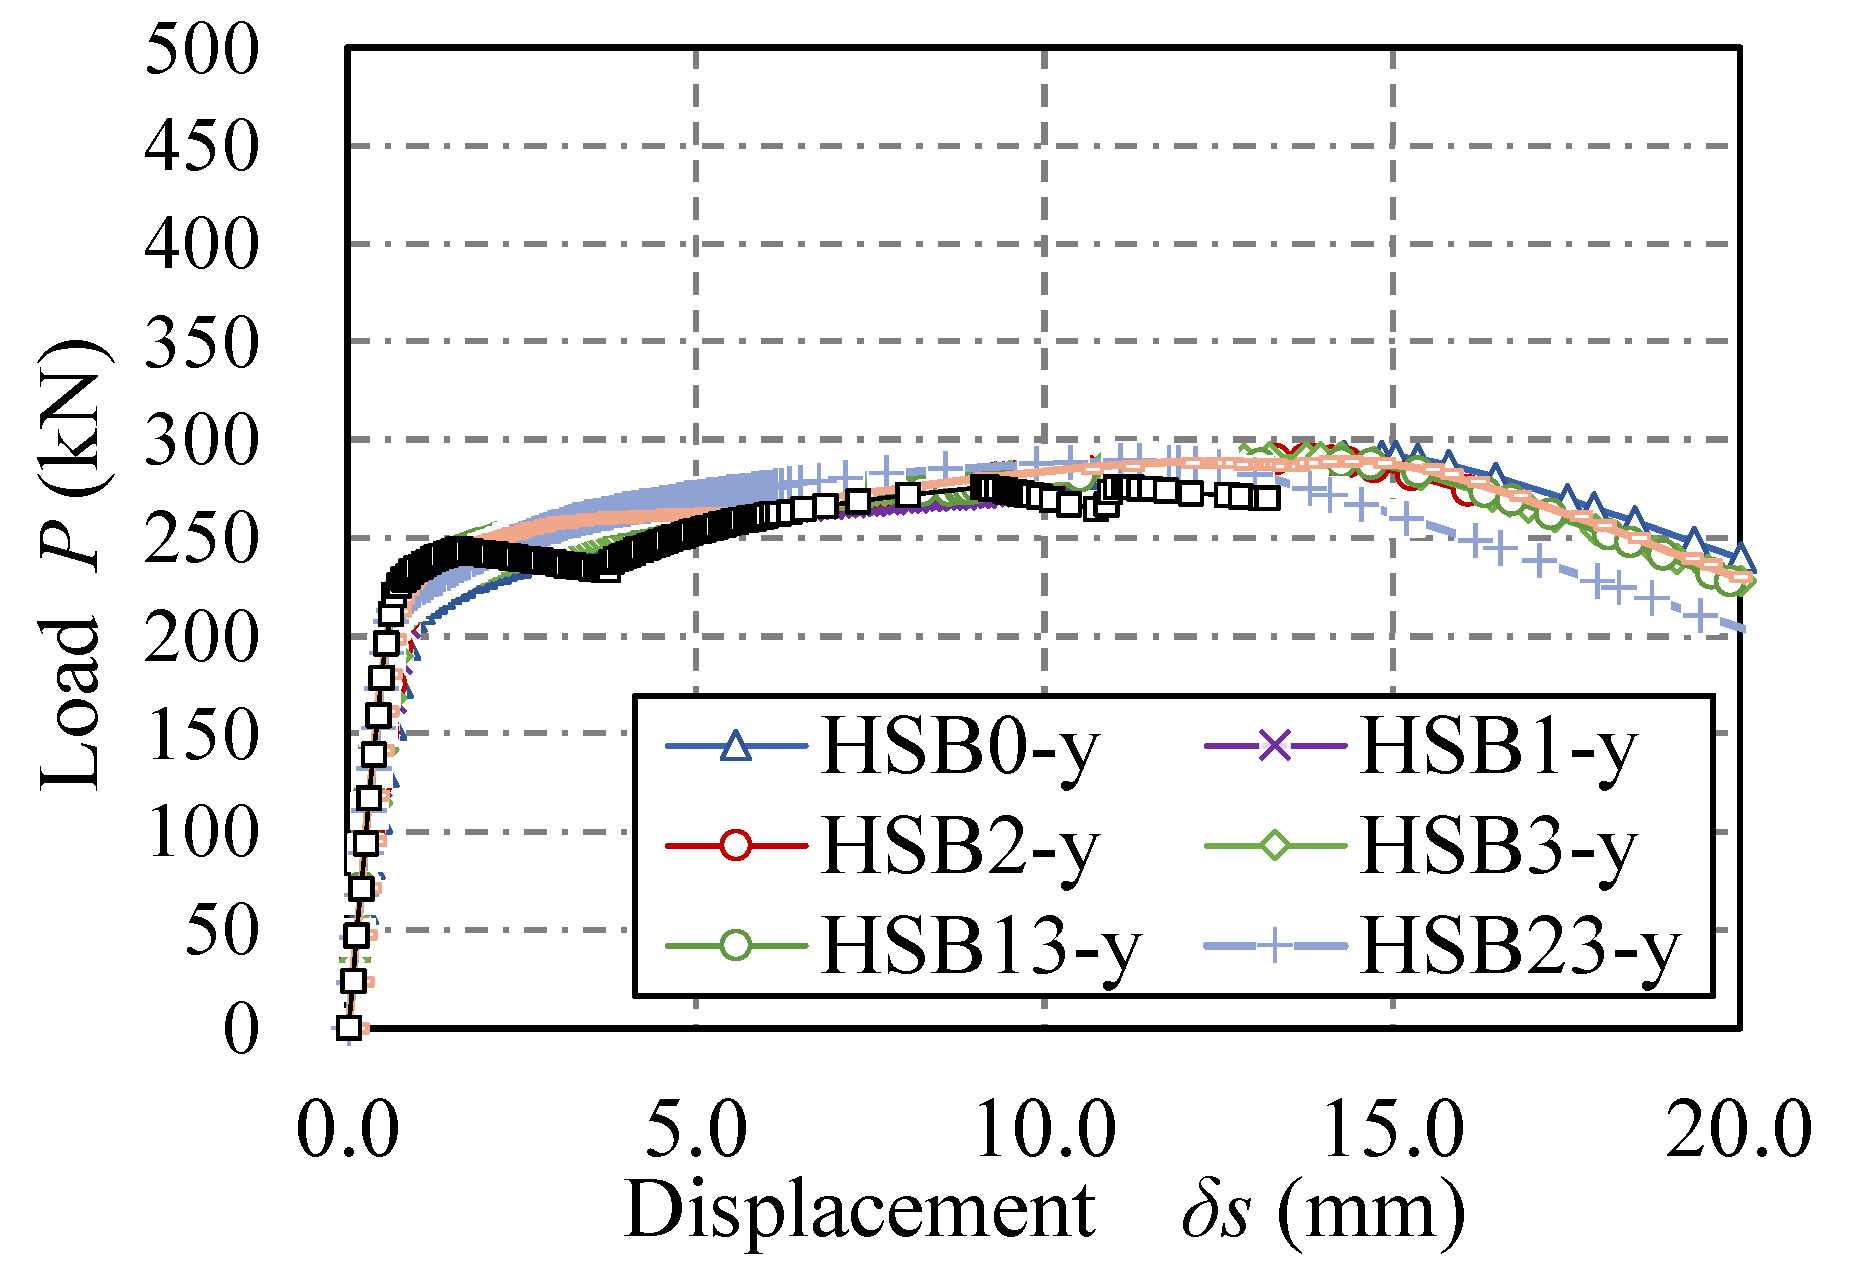
\includegraphics[width=\linewidth]{imgs/ch4/fig11-a.pdf}
    \caption{Overall}
    \label{ch4fig11-a}
    \end{subfigure}
    \begin{subfigure}[t]{0.48\textwidth}
    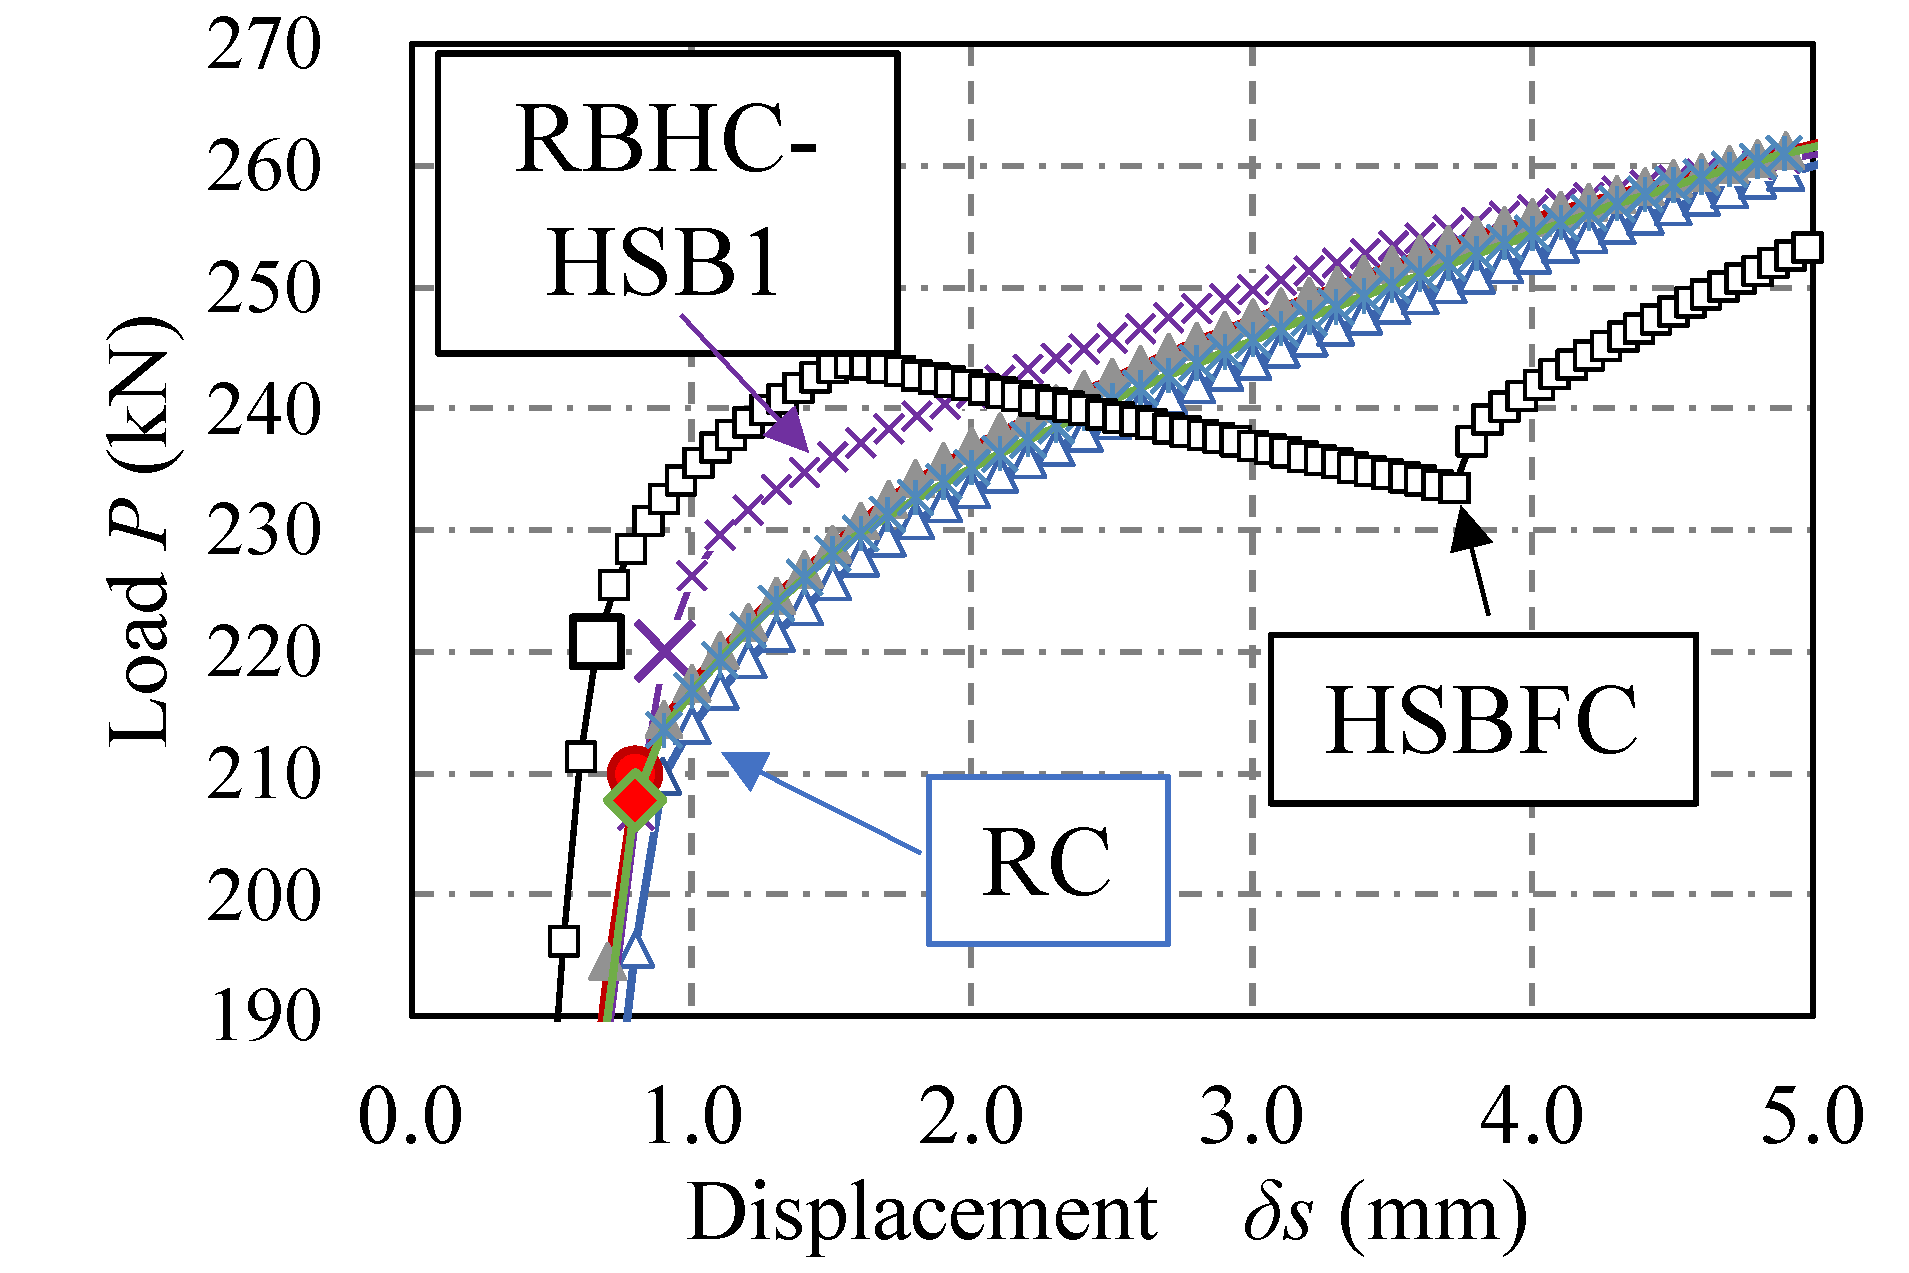
\includegraphics[width=\linewidth]{imgs/ch4/fig11-b.pdf}
    \caption{Enlarged figure ($n_b=1, n_r=2$)}
    \label{ch4fig11-b}
    \end{subfigure}
    \hfill
    \begin{subfigure}[t]{0.48\textwidth}
    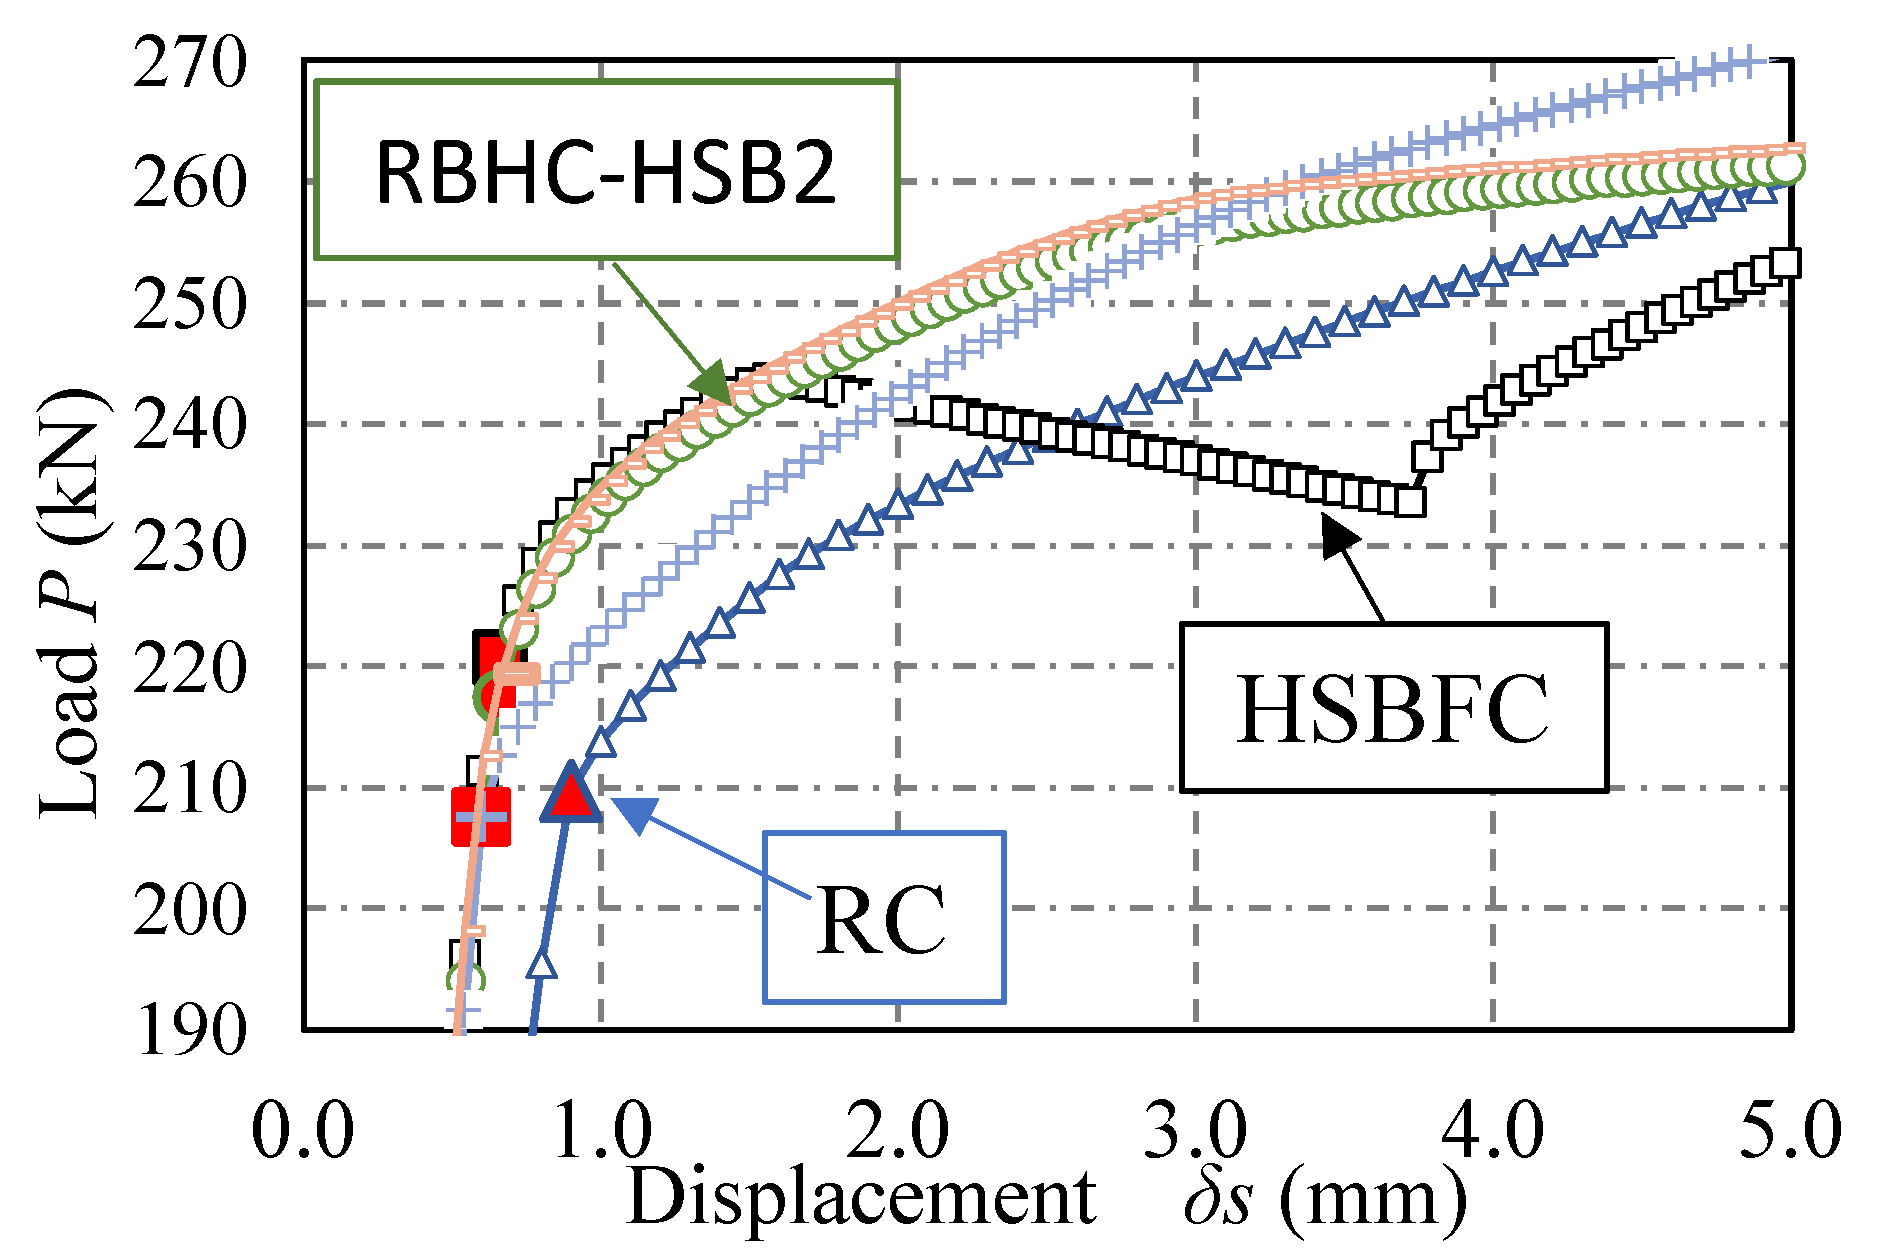
\includegraphics[width=\linewidth]{imgs/ch4/fig11-c.pdf}
    \caption{Enlarged figure ($n_b=2, n_r=1$)}
    \label{ch4fig11-c}
    \end{subfigure}
    \caption{Relationship between load and displacement (net cross-section yield first type)}
    \label{ch4fig11}
\end{figure}

\begin{figure}[htbp]
    \centering
    \begin{subfigure}[t]{0.76\textwidth}
    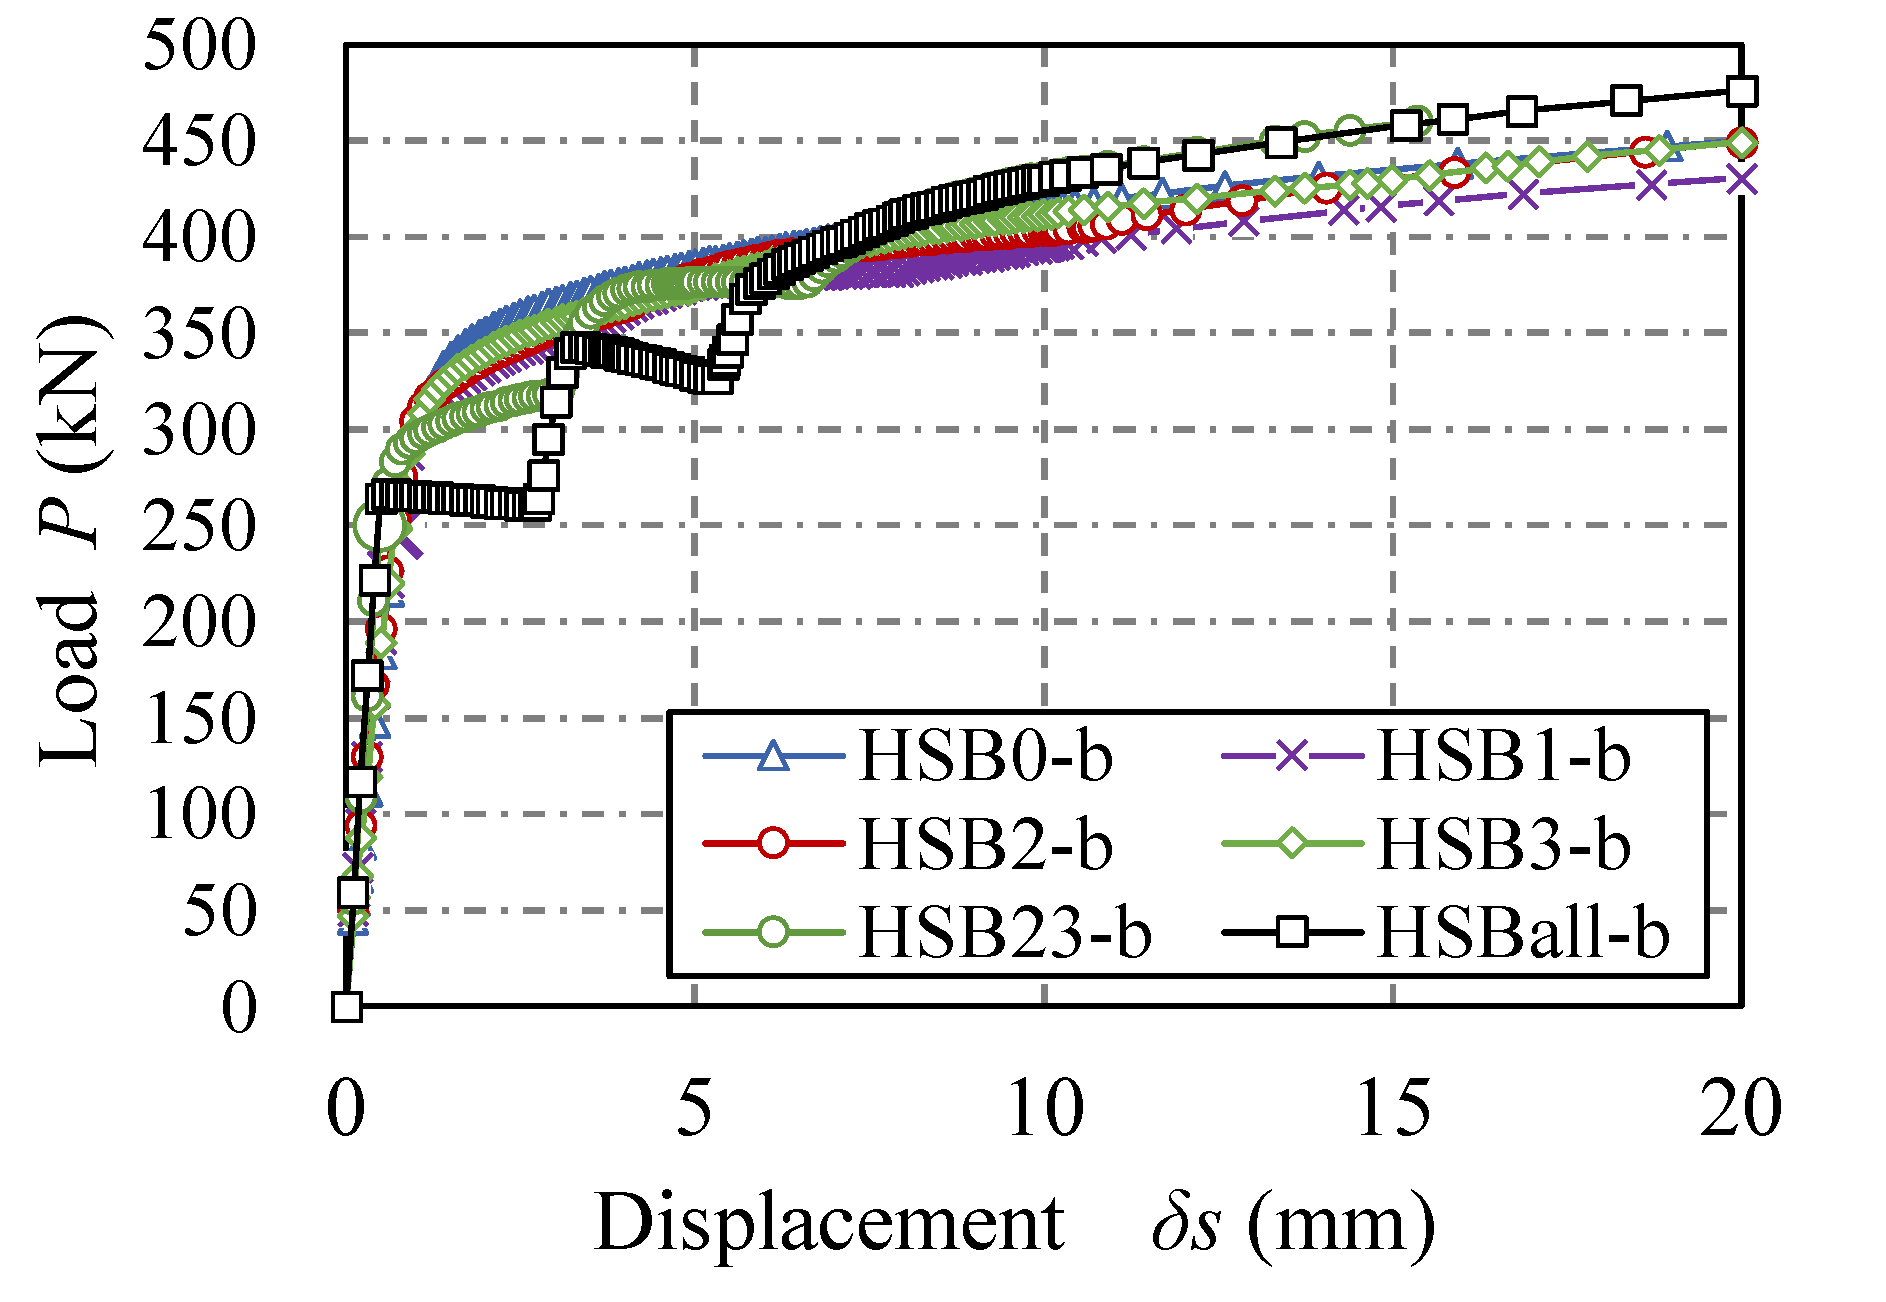
\includegraphics[width=\linewidth]{imgs/ch4/fig12-a.pdf}
    \caption{Overall}
    \label{ch4fig12-a}
    \end{subfigure}
    \begin{subfigure}[t]{0.48\textwidth}
    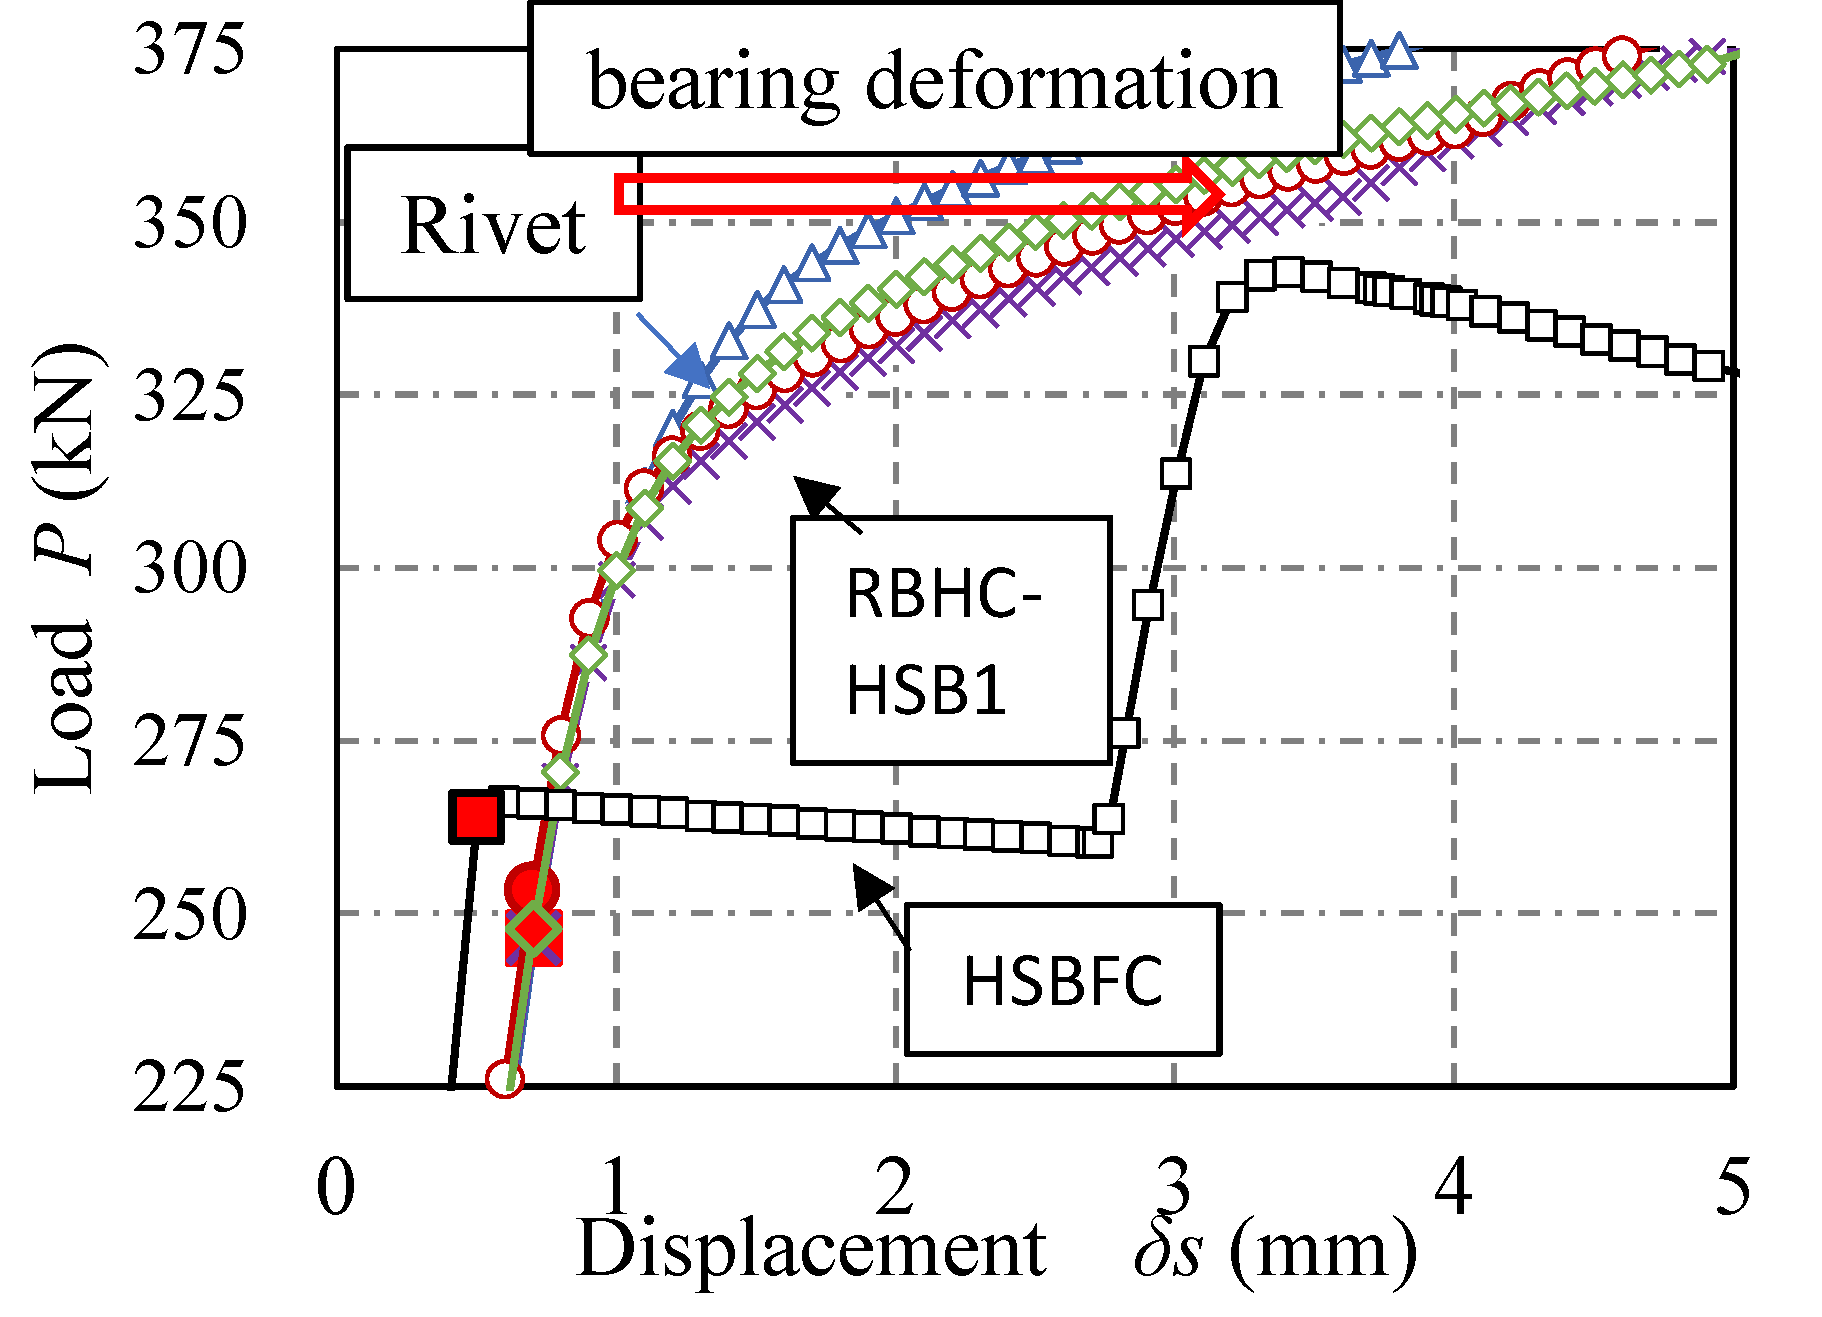
\includegraphics[width=\linewidth]{imgs/ch4/fig12-b.pdf}
    \caption{Enlarged figure ($n_b=1, n_r=2$)}
    \label{ch4fig12-b}
    \end{subfigure}
    \hfill
    \begin{subfigure}[t]{0.48\textwidth}
    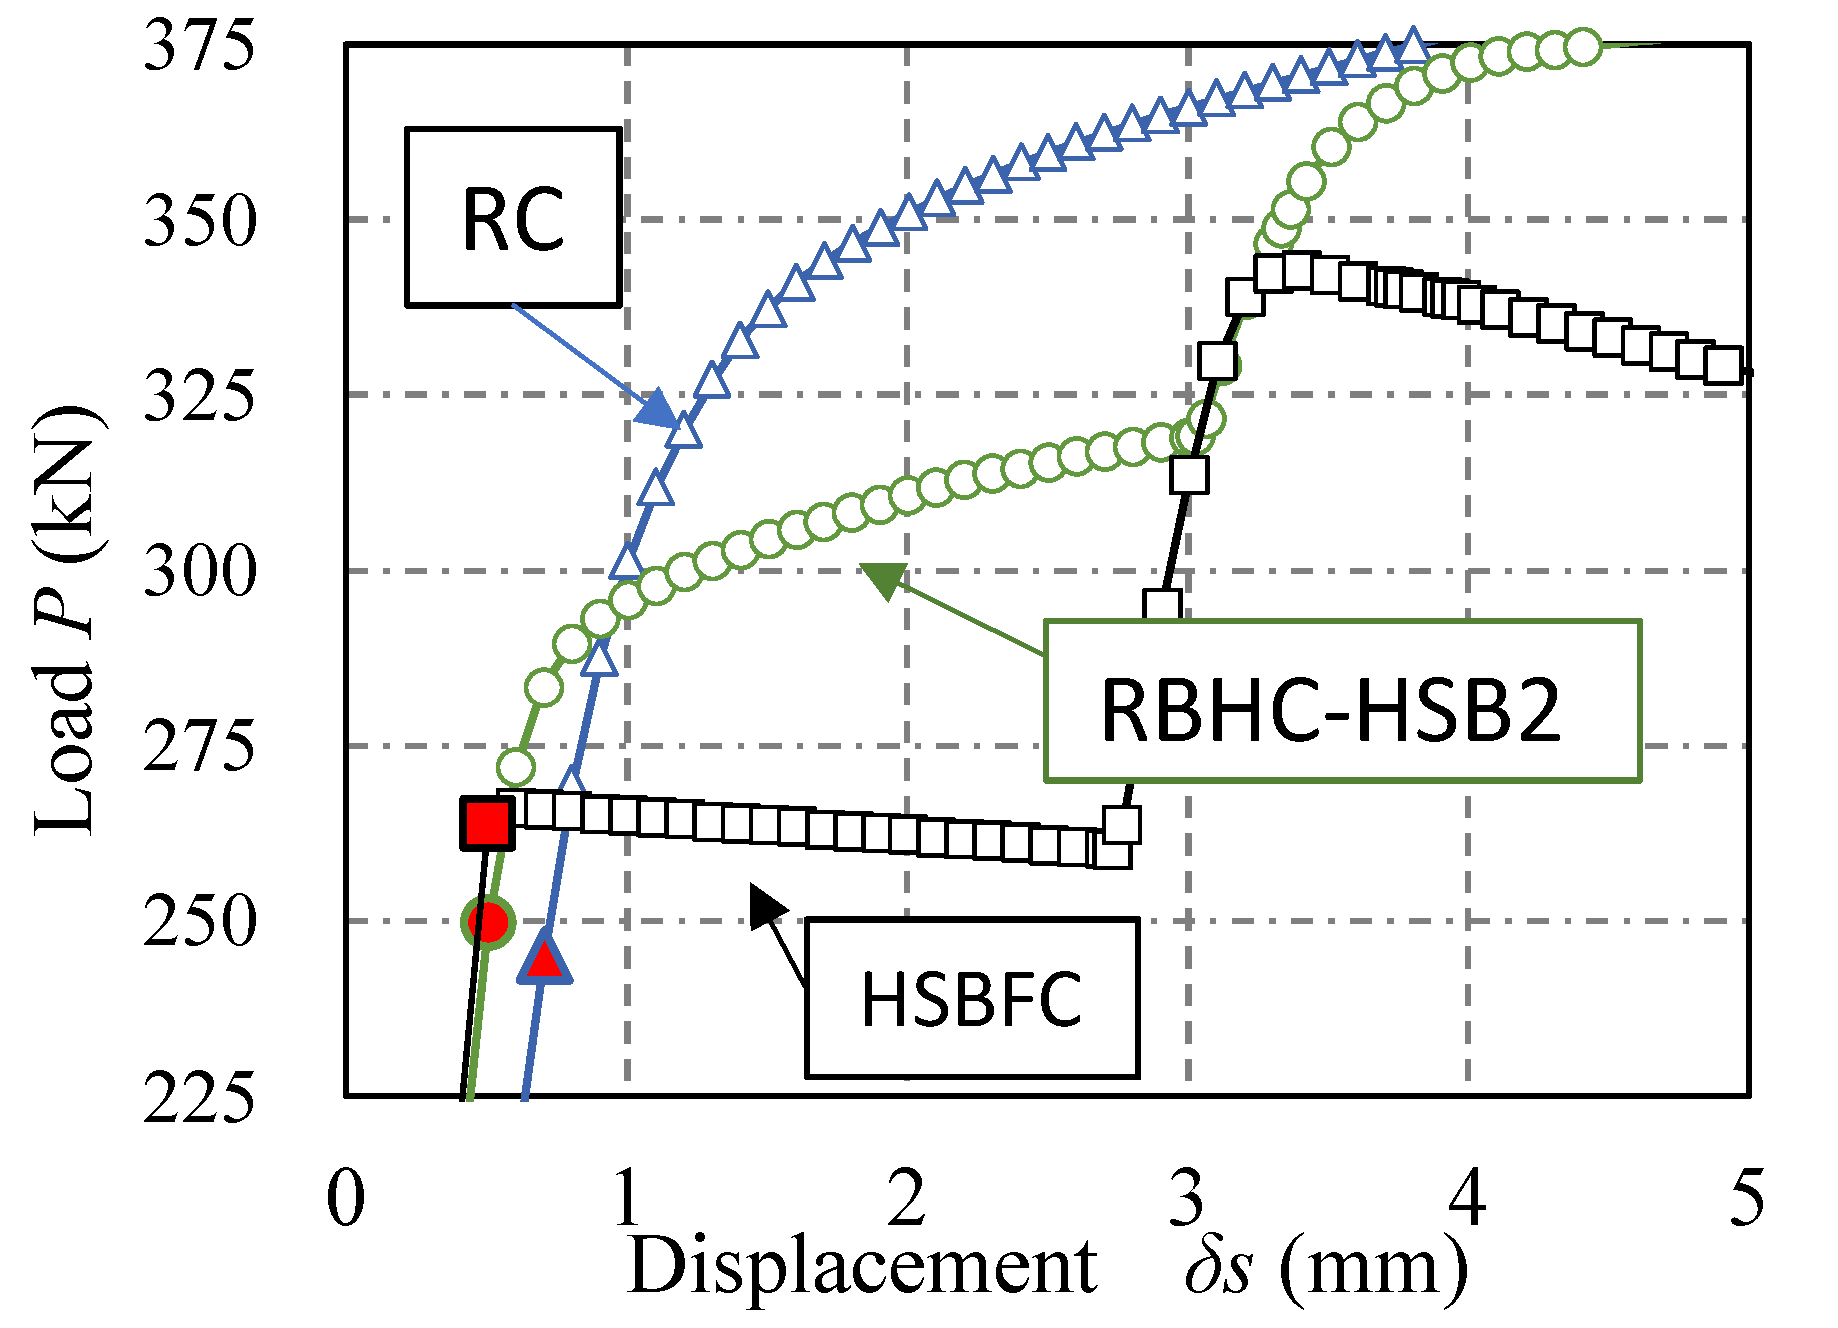
\includegraphics[width=\linewidth]{imgs/ch4/fig12-c.pdf}
    \caption{Enlarged figure ($n_b=2, n_r=1$)}
    \label{ch4fig12-c}
    \end{subfigure}
    \caption{Relationship between load and displacement (bearing yield first type)}
    \label{ch4fig12}
\end{figure}

The relationship between load and relative displacement for the net cross-section yield first and bearing yield first cases are shown in Fig. \ref{ch4fig13} and Fig. \ref{ch4fig14}, respectively. The relative displacement on the horizontal axis is the relative displacement in the direction of load between the bracing plate and the welded material at a position 10 mm from the edge of the welded material on the play side at the joint cover surface.

\subsubsection{Net section yield-precedence type}

Fig. \ref{ch4fig11} shows that the initial stiffness of the riveted joints (HSB0-y) is lower than that of the combined and friction joints (HSBall-y), and in all cases, net section yielding occurred at the point of initial stiffness change.

Fig. \ref{ch4fig11-b} shows that the load at the initial stiffness change point was the same for all cases with a single high-strength bolt (HSB1-y, 2-y, 3-y), but the slope of the curve after that point was larger for the case with the high-strength bolt placed at fastener position 1 (HSB1), the pure cross-section position. This is considered to be due to the fact that when the high-strength bolt is placed at fastener position 1, the load transfer by frictional force outside the pure cross-sectional position is larger.

Fig. \ref{ch4fig11-c} shows that the initial stiffness of the cases with two high-strength bolts (HSB13-y, 23-y, and 12-y) is the same as that of the HSB friction joint (HSBall-y). However, the initial stiffness change point and subsequent stiffnesses were lower for HSB-23-y, where only fastener position 1 was not replaced, than for the other cases with two high-strength bolts and HSBall-y. The behavior after pure sectional yielding showed that HSBall-y experienced a drop in load when the load was 243 $kN$. This was due to the preload loss of the high-strength bolt caused by pure section yielding, which resulted in slippage. However, for HSB13-y and HSB12-y, the slope change of the curve near the slip capacity was small because the load was transmitted by the support pressure of the rivets even after the slip capacity was exceeded.

Fig. \ref{ch4fig13} shows that the slope between load and relative displacement before the net section yield load was exceeded was the smallest for HSB0-y and was similar for HSBall-y and the combined joint. The initial relative displacement increment was smaller for the combined joints when the high-strength bolt was used as the fastener closer to the location where the relative displacement was obtained.

\begin{figure}[htbp]
    \centering
    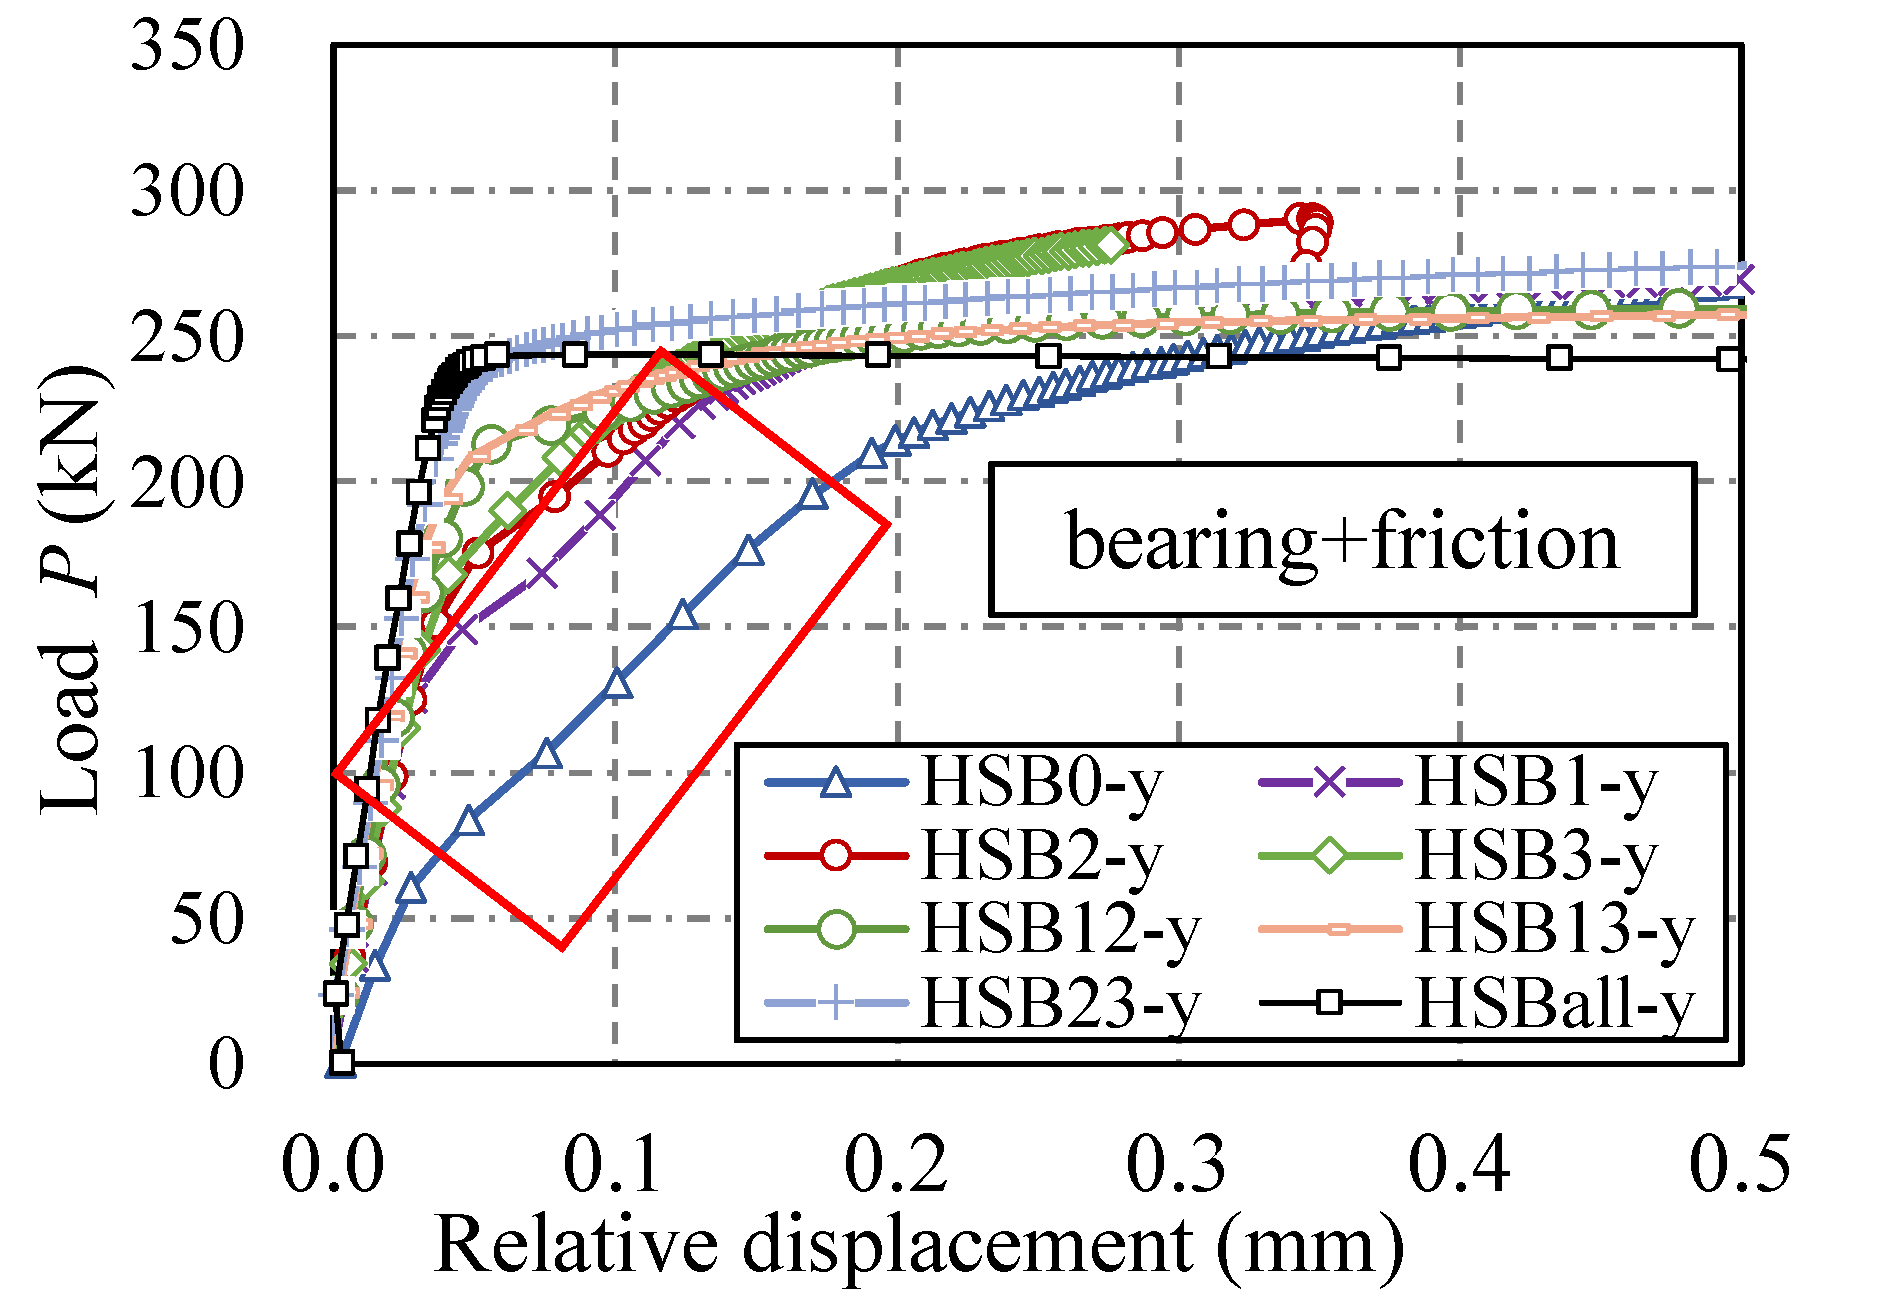
\includegraphics[width=0.75\textwidth]{imgs/ch4/fig13.pdf}
    \caption{Relationship between load and relative displacement (net cross-section yield first type)}
    \label{ch4fig13}
\end{figure}

\subsubsection{Bearing yield type}

Fig. \ref{ch4fig12} shows that the initial stiffness of the case with two high-strength bolts (HSB23-b) was similar to that of the friction-jointed HSBall-b. For HSBall-b, the displacement increased while the load decreased at 263.7 $kN$, and the analytical values generally agreed with the sliding capacity, Fslip  = 258.3 $kN$. In the case of the combined joint, the load increased even when the slip capacity was exceeded, and the displacement increment was small.

From Fig. \ref{ch4fig12-b}, \ref{ch4fig12-c}, the curves after exceeding the bearing pressure load $P_{bya}$ (indicated by the larger plots) (overall displacement of 1mm~3mm) were at the top for the riveted joint (HSB0-b) and at the bottom for the HSB23-b case. This is because there are three rivets resisting bearing pressure in the riveted joints, and in the HSB23-b case, the load is resisted by the bearing pressure of one rivet and the friction of two high-strength bolts before the high-strength bolts enter the bearing pressure.

Fig. \ref{ch4fig14} shows that in all cases, the point of change in the slope of the curve of the relative displacement-load relationship (indicated by the large plot) was equivalent to the slip capacity Fslip . In addition, HSBall-b, which was frictionally joined with high-strength bolts, exhibited clear slippage, while the other joints with rivets did not exhibit slippage.

\begin{figure}[htbp]
    \centering
    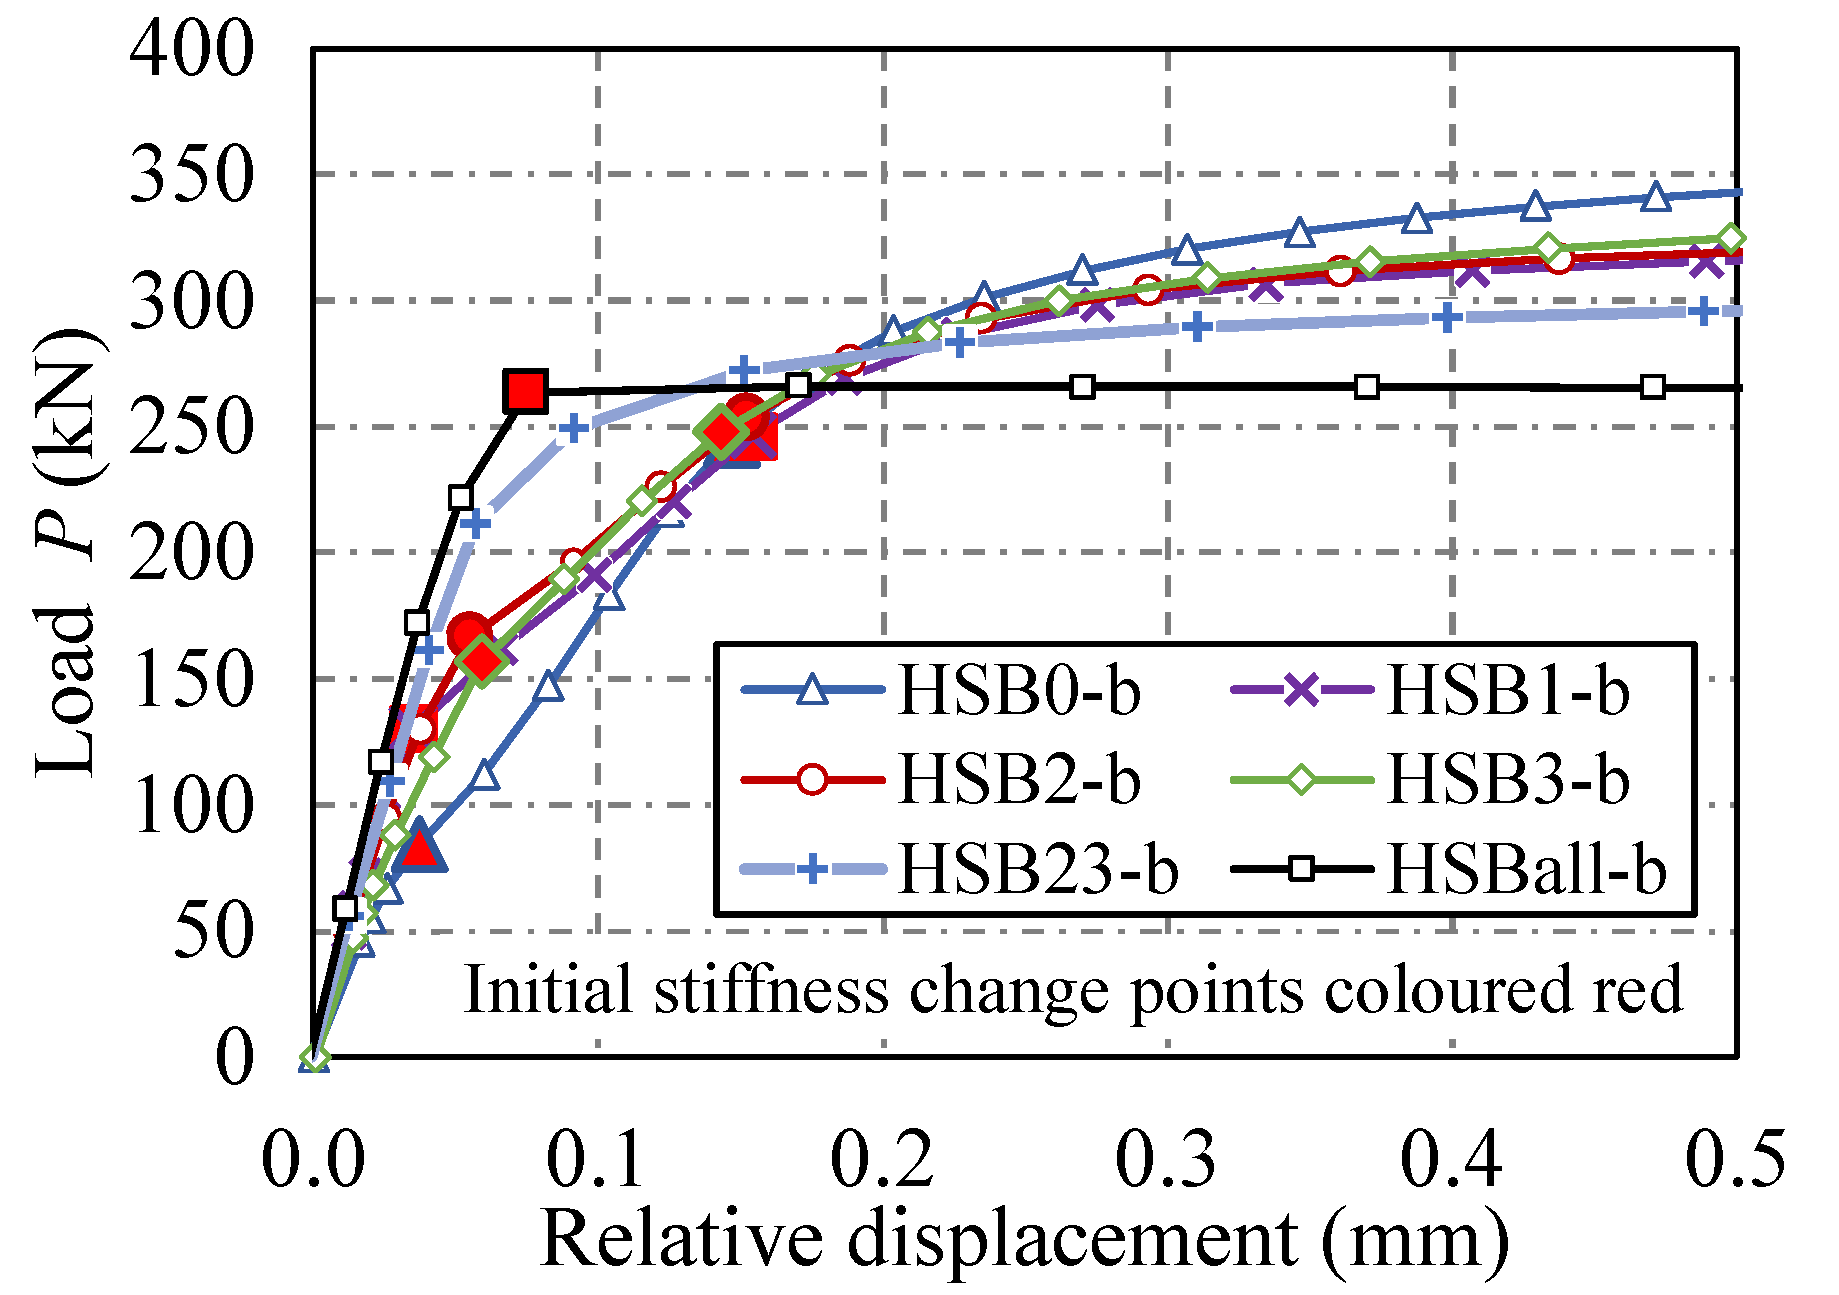
\includegraphics[width=0.75\textwidth]{imgs/ch4/fig14.pdf}
    \caption{Relationship between load and relative displacement (bearing yield first type)}
    \label{ch4fig14}
\end{figure}

\subsubsection{Load Transfer Mechanism}

As shown in Fig. \ref{ch4fig15}, the combined joint transmits loads through three processes: (1) a friction transmission phase in which loads are transmitted almost exclusively by friction up to a slip capacity $F_{slip}$ , (2) a combined transmission phase in which loads are transmitted by bearing pressure and friction up to a bearing load $P_{bya}$ , and (3) a plastic deformation phase in which the joint is plastically deformed afterwards.

\begin{figure}[htbp]
    \centering
    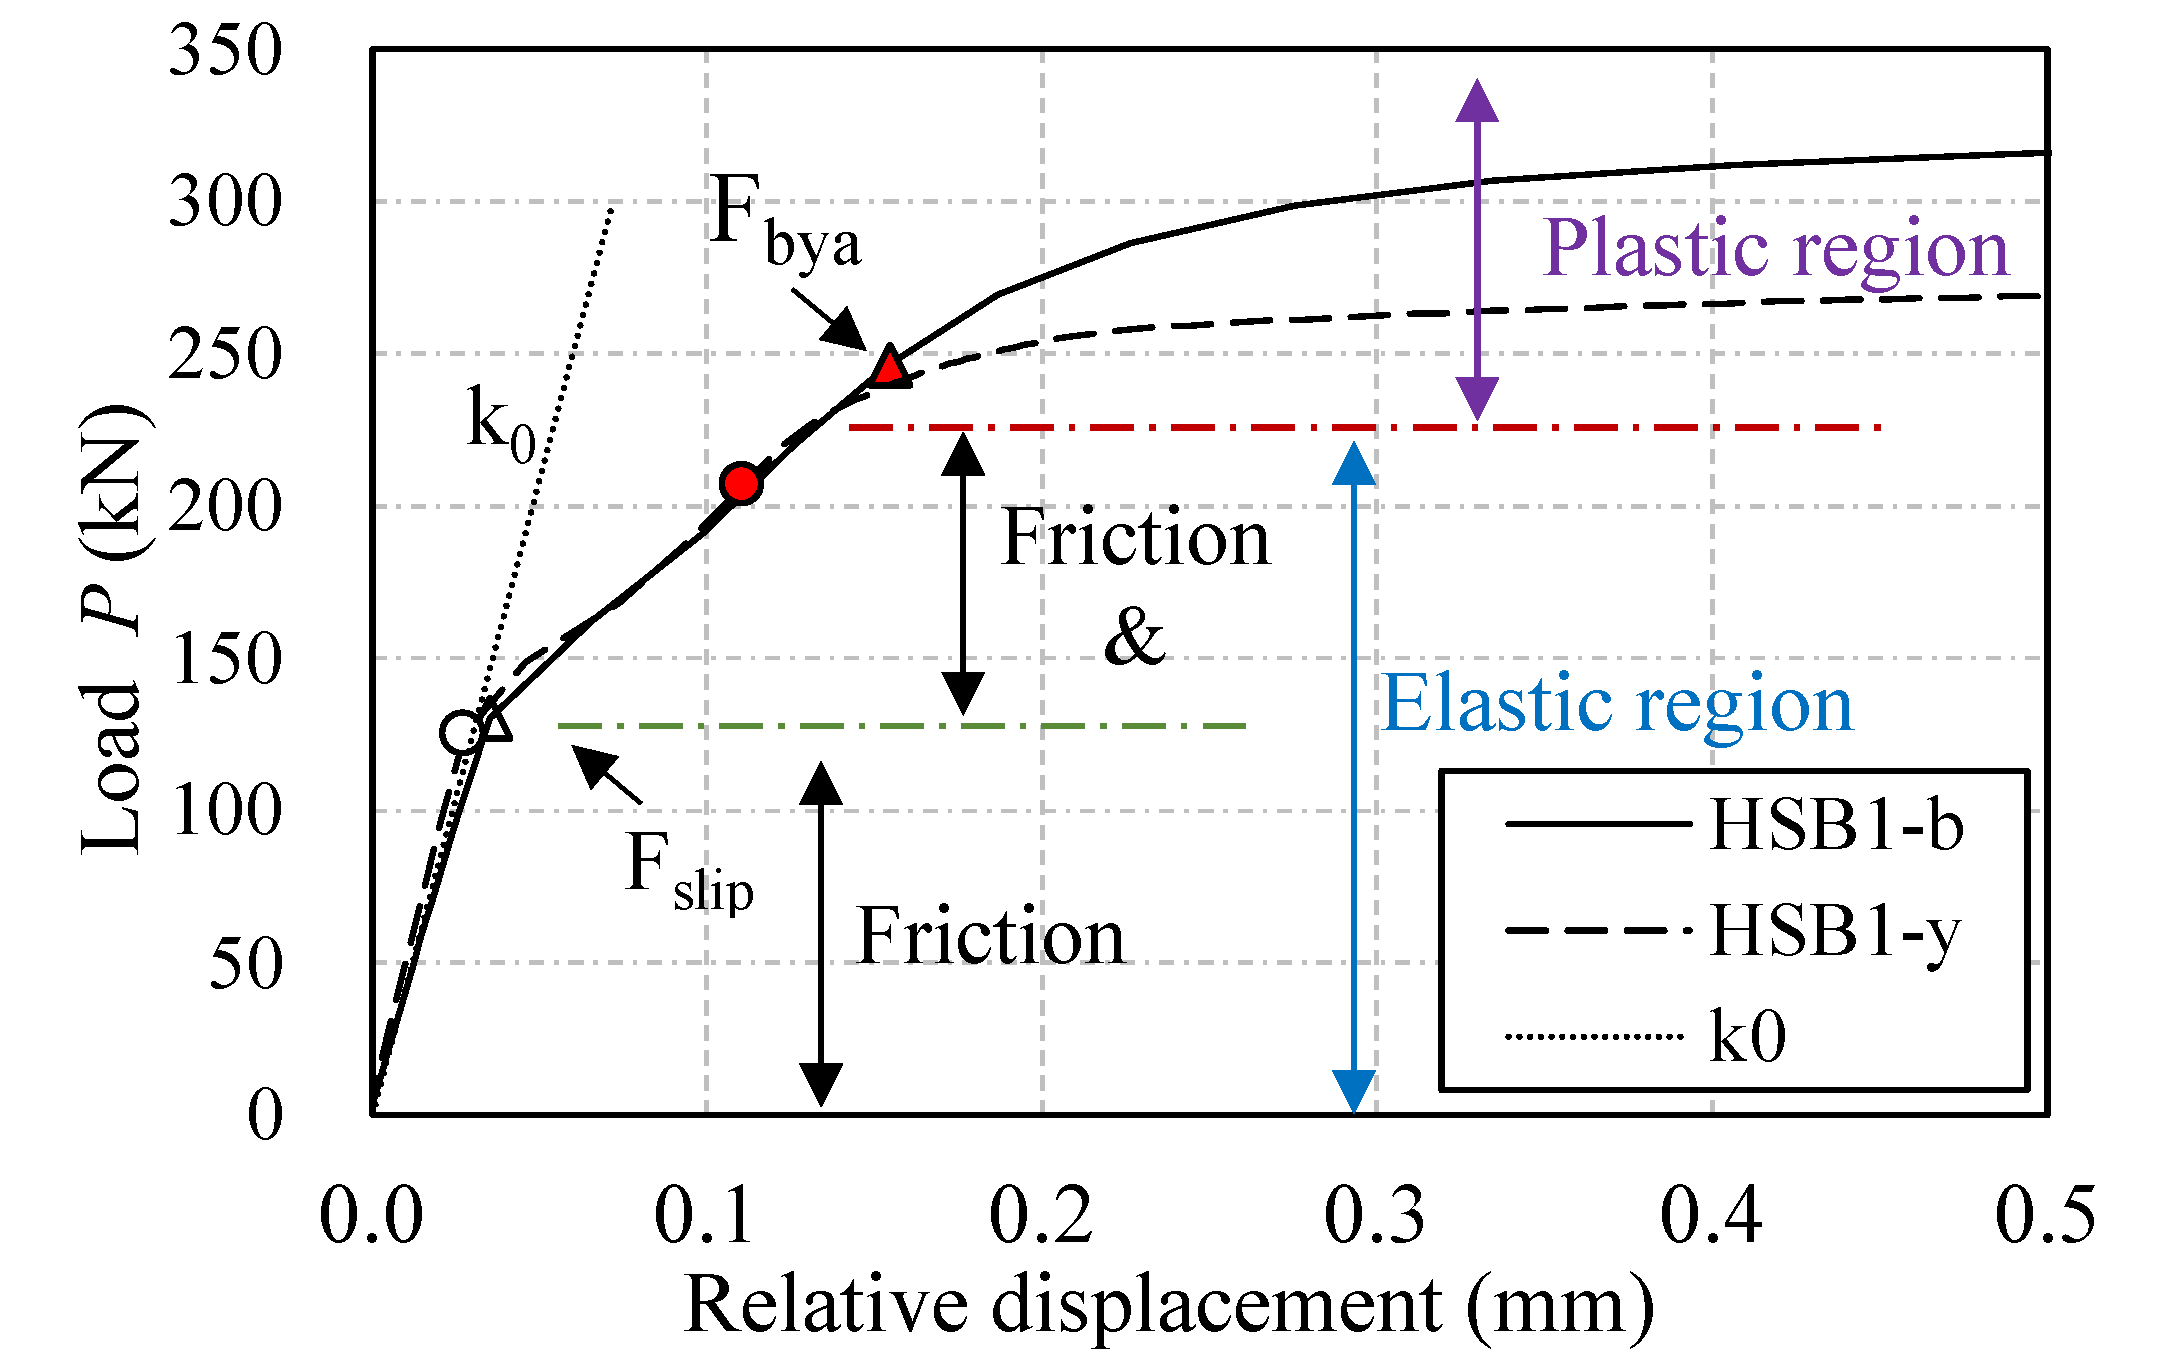
\includegraphics[width=0.85\textwidth]{imgs/ch4/fig15.pdf}
    \caption{Schematic diagram of a hybrid joint.}
    \label{ch4fig15}
\end{figure}

The initial stiffness is determined in the friction transfer phase. The slope of the curve in the combined transfer phase is constant, although it is less than the initial stiffness, and represents the elastic behavior in the bearing state. The slope of the curve then changes and exhibits non-linearity when the bearing load $P_{bya}$ is exceeded in the case of the pressure-precedence type and when the net sectional yield load Fy is exceeded in the case of the yield-precedence type. This is considered to be due to the development of plasticization in the bearing state or plasticization in the entire width direction of the net cross-sectional position.

Fig. \ref{ch4fig16} shows the dimensionless load-over-full displacement relationship for the pressure-precedence and pure-section yield-precedence types of combined joints. The vertical axis is non-dimensionalized using the analytical load Fa , which is the minimum value of the net section yield load, slip load, and bearing load in each case obtained from the analysis.

\begin{figure}[htbp]
    \centering
    \begin{minipage}[t]{0.48\textwidth}
    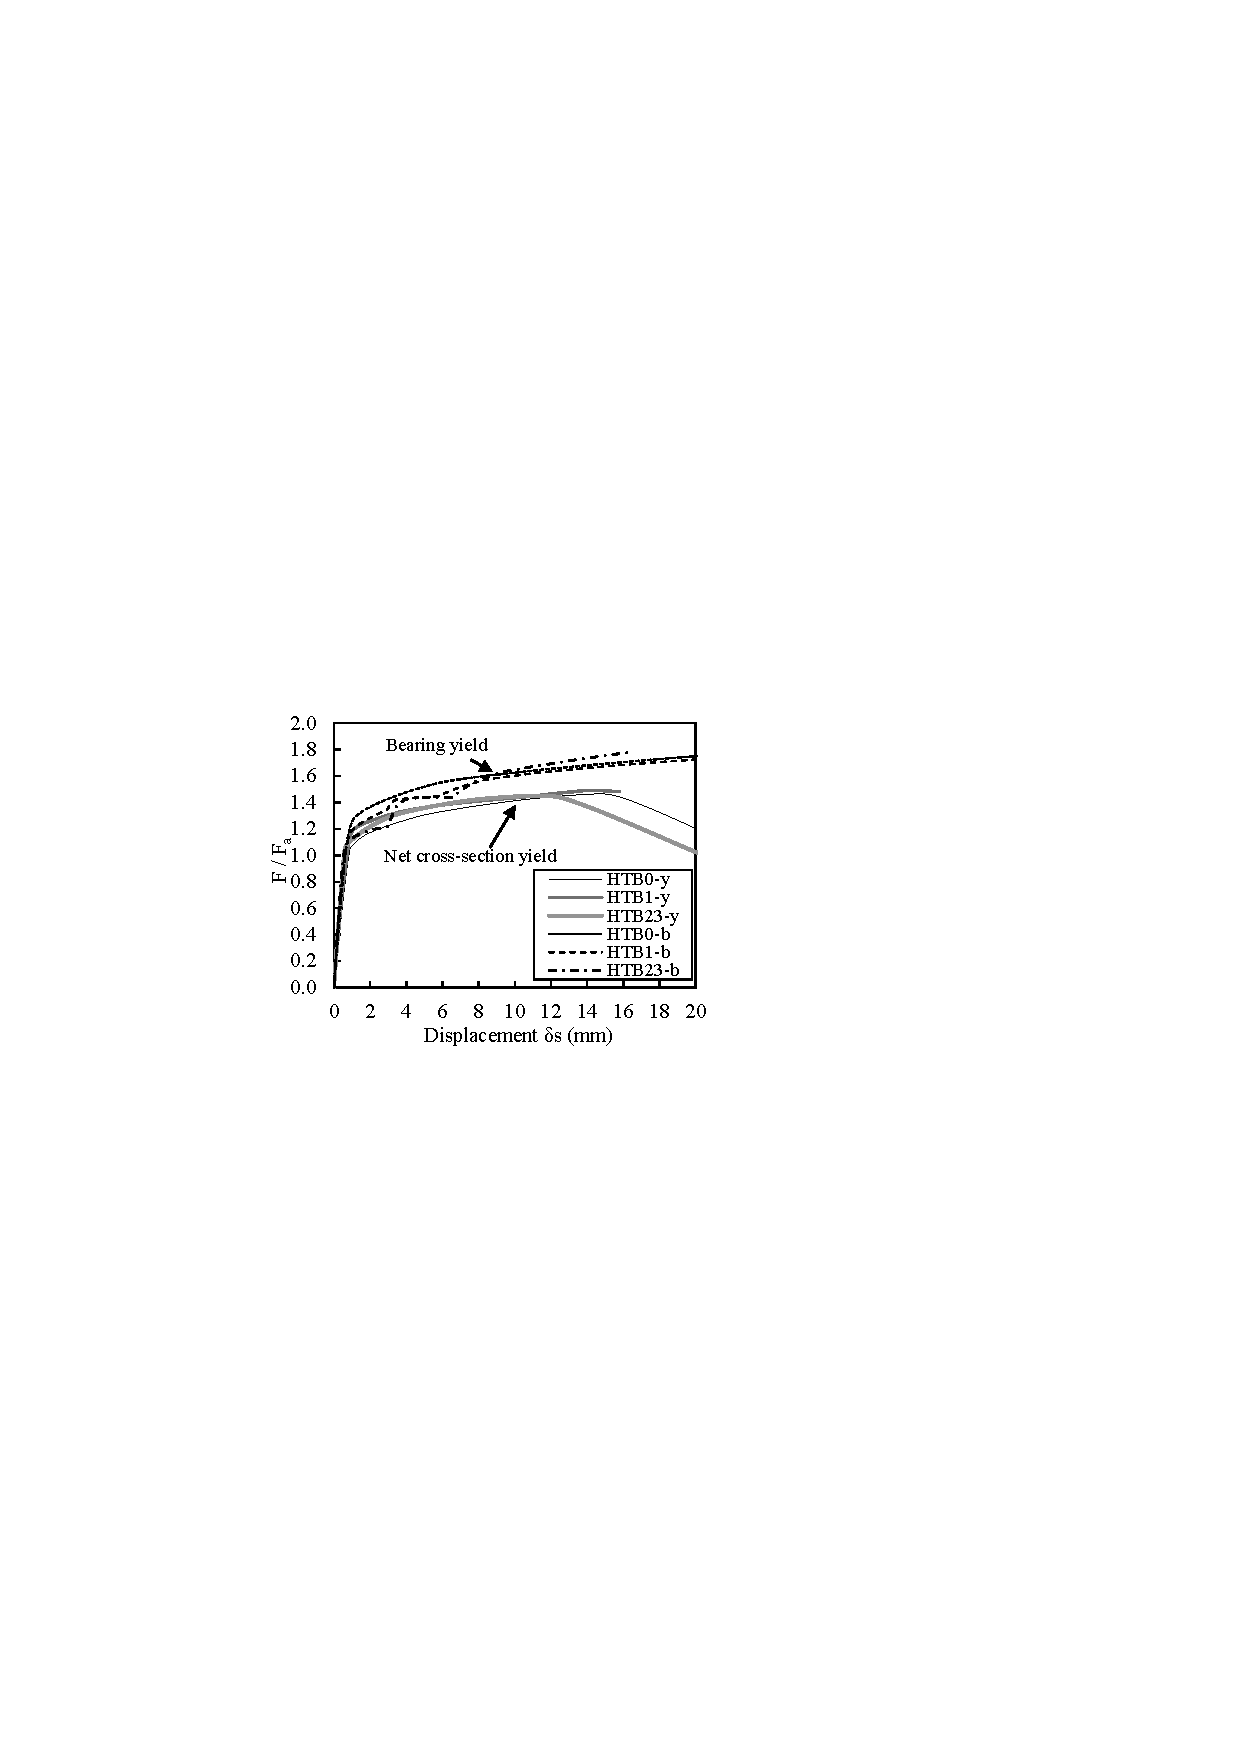
\includegraphics[width=\linewidth]{imgs/ch4/fig16.pdf}
    \caption{Relationship between load and overall displacement}
    \label{ch4fig16}
    \end{minipage}
    \begin{minipage}[t]{0.48\textwidth}
    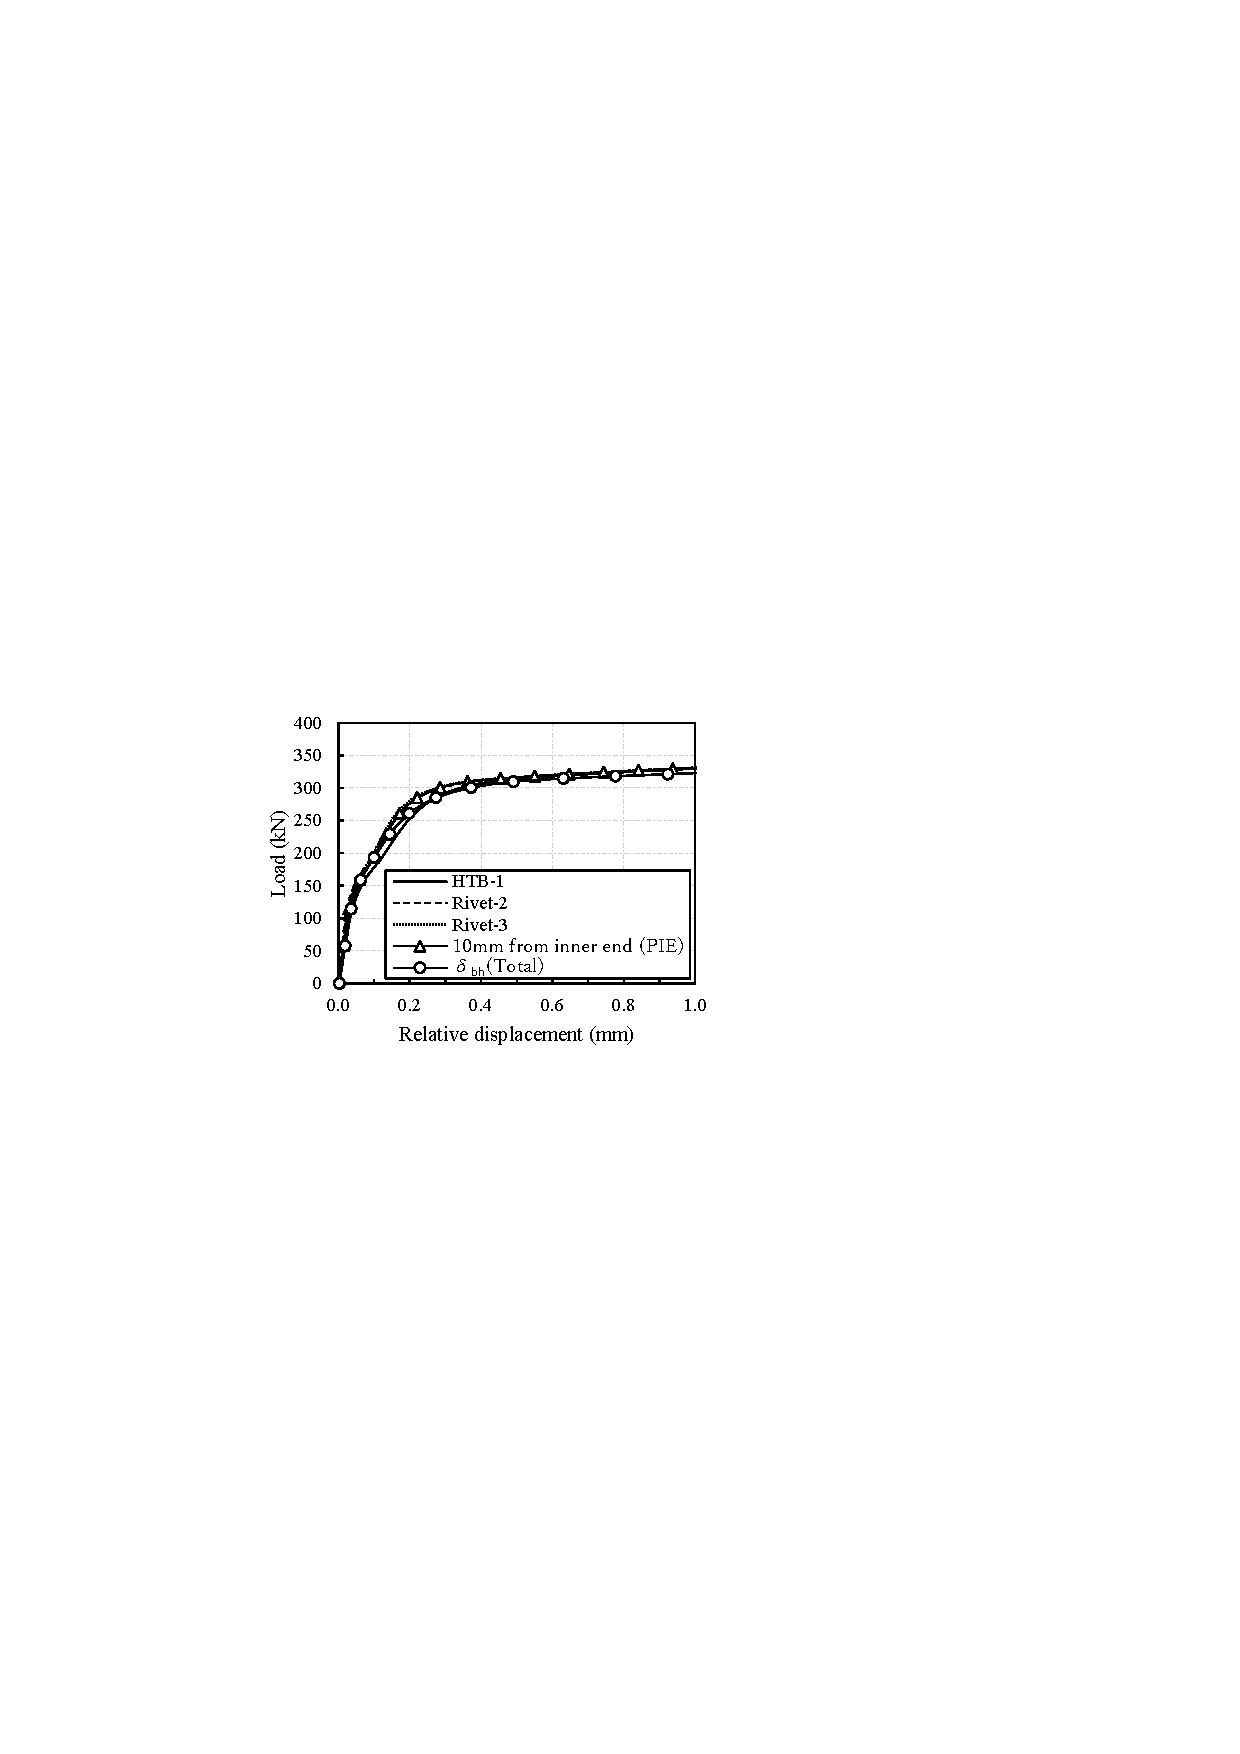
\includegraphics[width=\linewidth]{imgs/ch4/fig17.pdf}
    \caption{Relationship between load and the relative displacement of each position}
    \label{ch4fig17}
    \end{minipage}
\end{figure}

Fig. \ref{ch4fig16} shows that the slope of the curve after F / Fa = 1 is higher for the support-precedence type than for the pure-section yield-precedence type. The amount of elongation is relatively small because the deformation of the pure section yield-precedence type is localized until the maximum load is reached.

Fig. \ref{ch4fig17} shows the relationship between local relative deformation and load for HSB1-b. HSB-1, Rivet-2, and Rivet-3 show the relative displacement of the bonding plate and the bonded material at the center position of the fastener on each of the cover surfaces. The hole deformation (total) shows the sum of the hole deformations of all fastener holes.

Fig. \ref{ch4fig17} shows that the relative displacements of the contact plate and the welded material at the center of each fastener were about the same, which confirms that no localized slippage occurred. The relative displacement at 10 mm from the edge of the joint is almost equal to the sum of the hole deformation, and it can be judged that the amount of support deformation and relative displacement of the joint behaves almost the same. In other cases, the results were similar to those of HSB1.

This indicates that the combined riveted and high-strength bolted friction joints do not exhibit slip and that the relative deformation calculated from the hole deformation of the joint and the main plate due to support deformation is the same as the relative displacement calculated from the displacement of the jointed plate and the main plate's cover surfaces. It can be inferred that unless net sectional yielding occurs, the amount of support deformation in a combination joint can be calculated from the relative displacement of the joint cover surfaces.
3.3 Load Sharing of Combined Joints

In order to focus on the load transfer sharing between bearing pressure and friction in a combined joint, the case of a bearing pressure-precedence type, in which the effect of net sectional yielding is small, is considered.

Fig. \ref{ch4fig18} shows the load sharing at ratios F / $P_{bya}$ = 0.25, 0.5, 1 for tensile load F and bearing load $P_{bya}$ . The hole deformation in the loading direction at F / $P_{bya}$ = 0.5, 1 is shown in Figure 19. The bearing resistance force is the contact force between the fastener shaft and the fastener hole in the material to be joined in the load direction, and the friction resistance force is the shear friction force acting on the contact surface between the bracing plate and the material to be joined. It is confirmed that the total force of bearing resistance and friction resistance is equal to the total load.

\begin{figure}[htbp]
    \centering
    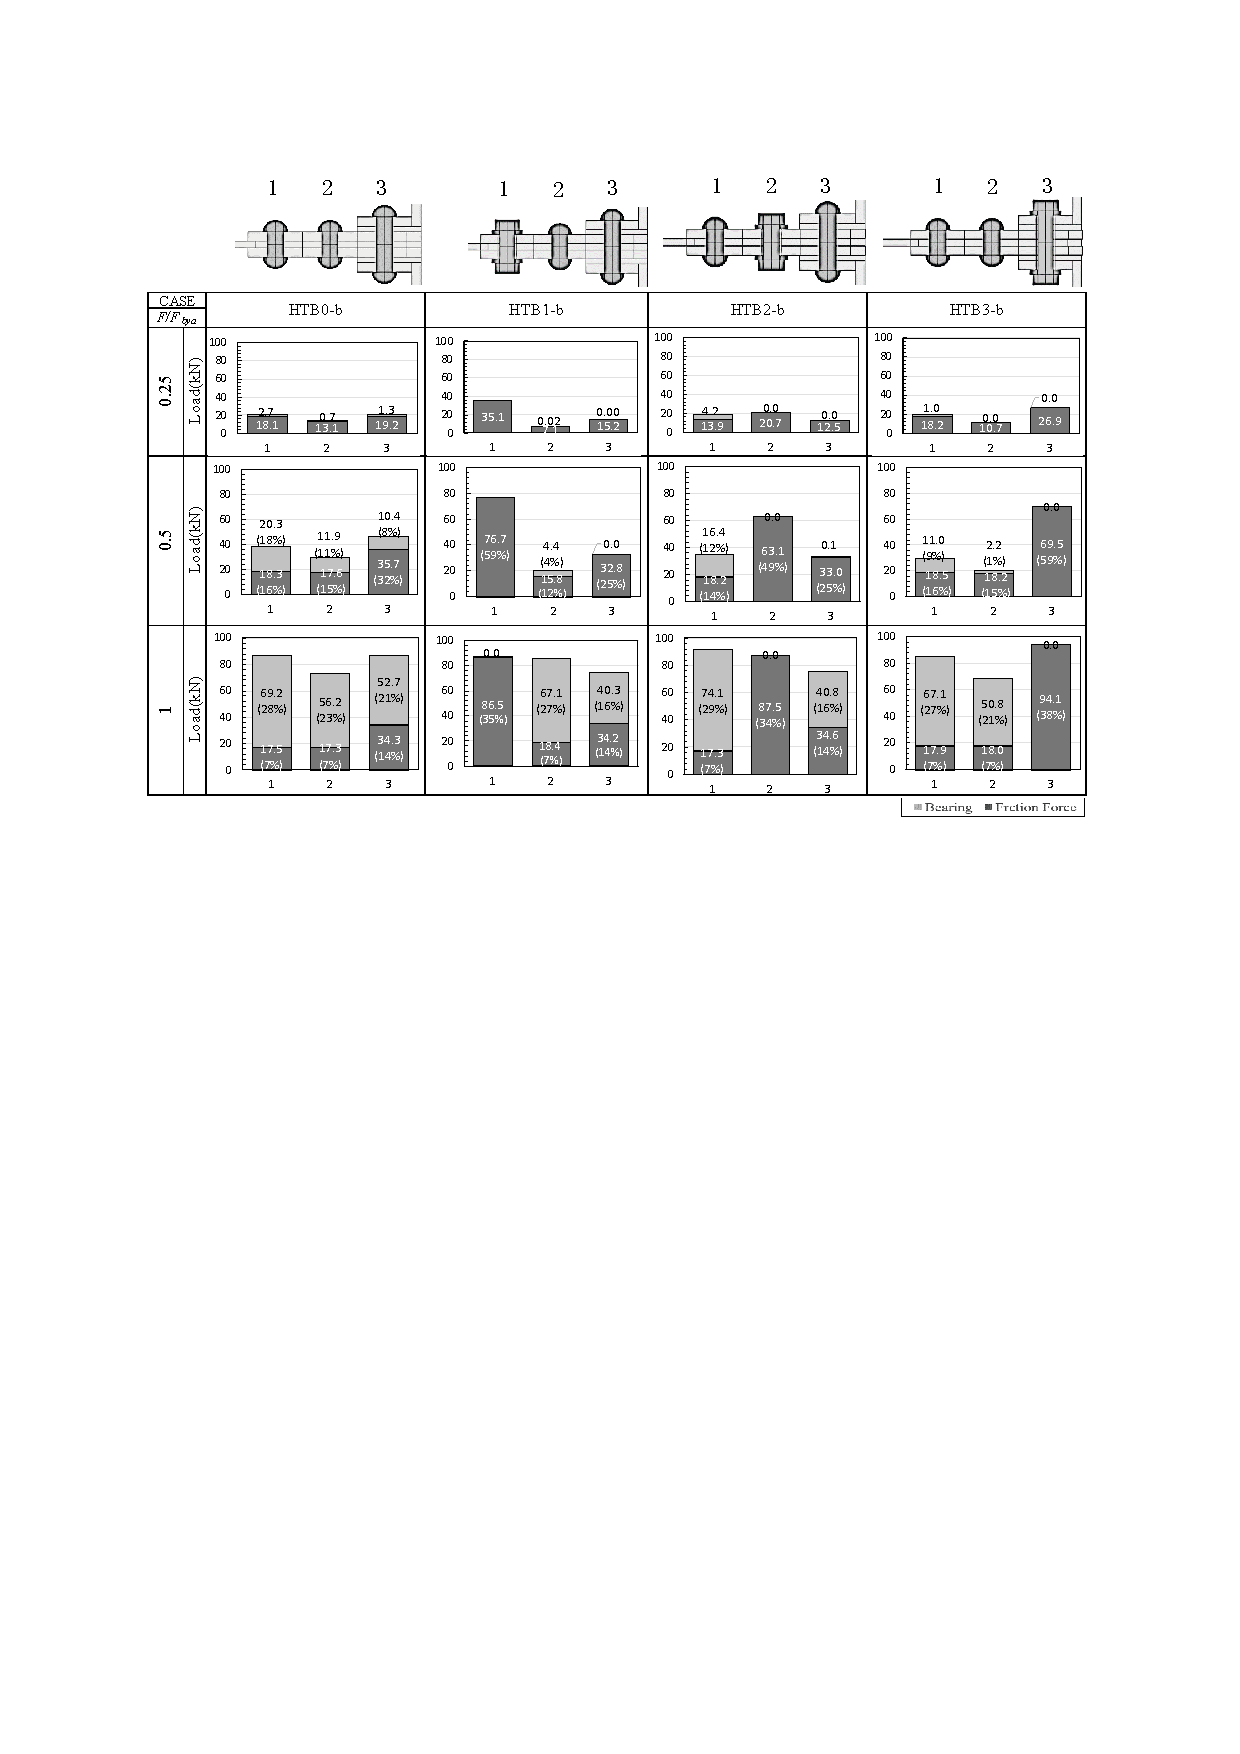
\includegraphics[width=\textwidth]{imgs/ch4/fig18.pdf}
    \caption{Load sharing of each case (bearing yield first type)}
    \label{ch4fig18}
\end{figure}

Fig. \ref{ch4fig18} shows that when F / $P_{bya}$ = 0.25, the riveted and combined joints resisted almost entirely by friction, and the load sharing increased when the high-strength bolt was placed outside the joint, with HSB1-b sharing 35.1 $kN$ (more than half the total load), HSB2-b 20.7 $kN$ (less than half the total load) and HSB3-b HSB3-b shared about 45\% of the total load. The load-bearing capacity of HSB2-b was 20.7 $kN$ (more than half of the total load) and that of HSB3-b was about 45\%.

When F / $P_{bya}$ = 0.5, cases HSB2-b and HSB3-b without a high-strength bolt at fastener position 1 resisted 16.4\% and 11\% of the total load, respectively, but in both cases most of the bearing pressure was shared by the rivets at outer fastener position 1. On the other hand, the load sharing for HSB1-b was the same, F / P = 0.25. When a high-strength bolt was placed at fastener position 1 in the support-precedence type, the support pressure of the rivets did not carry most of the load, and the load was shared through the frictional force of each fastener.

When F / $P_{bya}$  = 1, each fastener exceeded the slip capacity per fastener in all cases. In addition, the load carried by fastener position 1 was about 35\% of the total load, and the load carried by each fastener was almost equally distributed. The friction of the high-strength bolts and the bearing pressure of the rivets worked together to resist the load.

\begin{figure}[htbp]
    \centering
    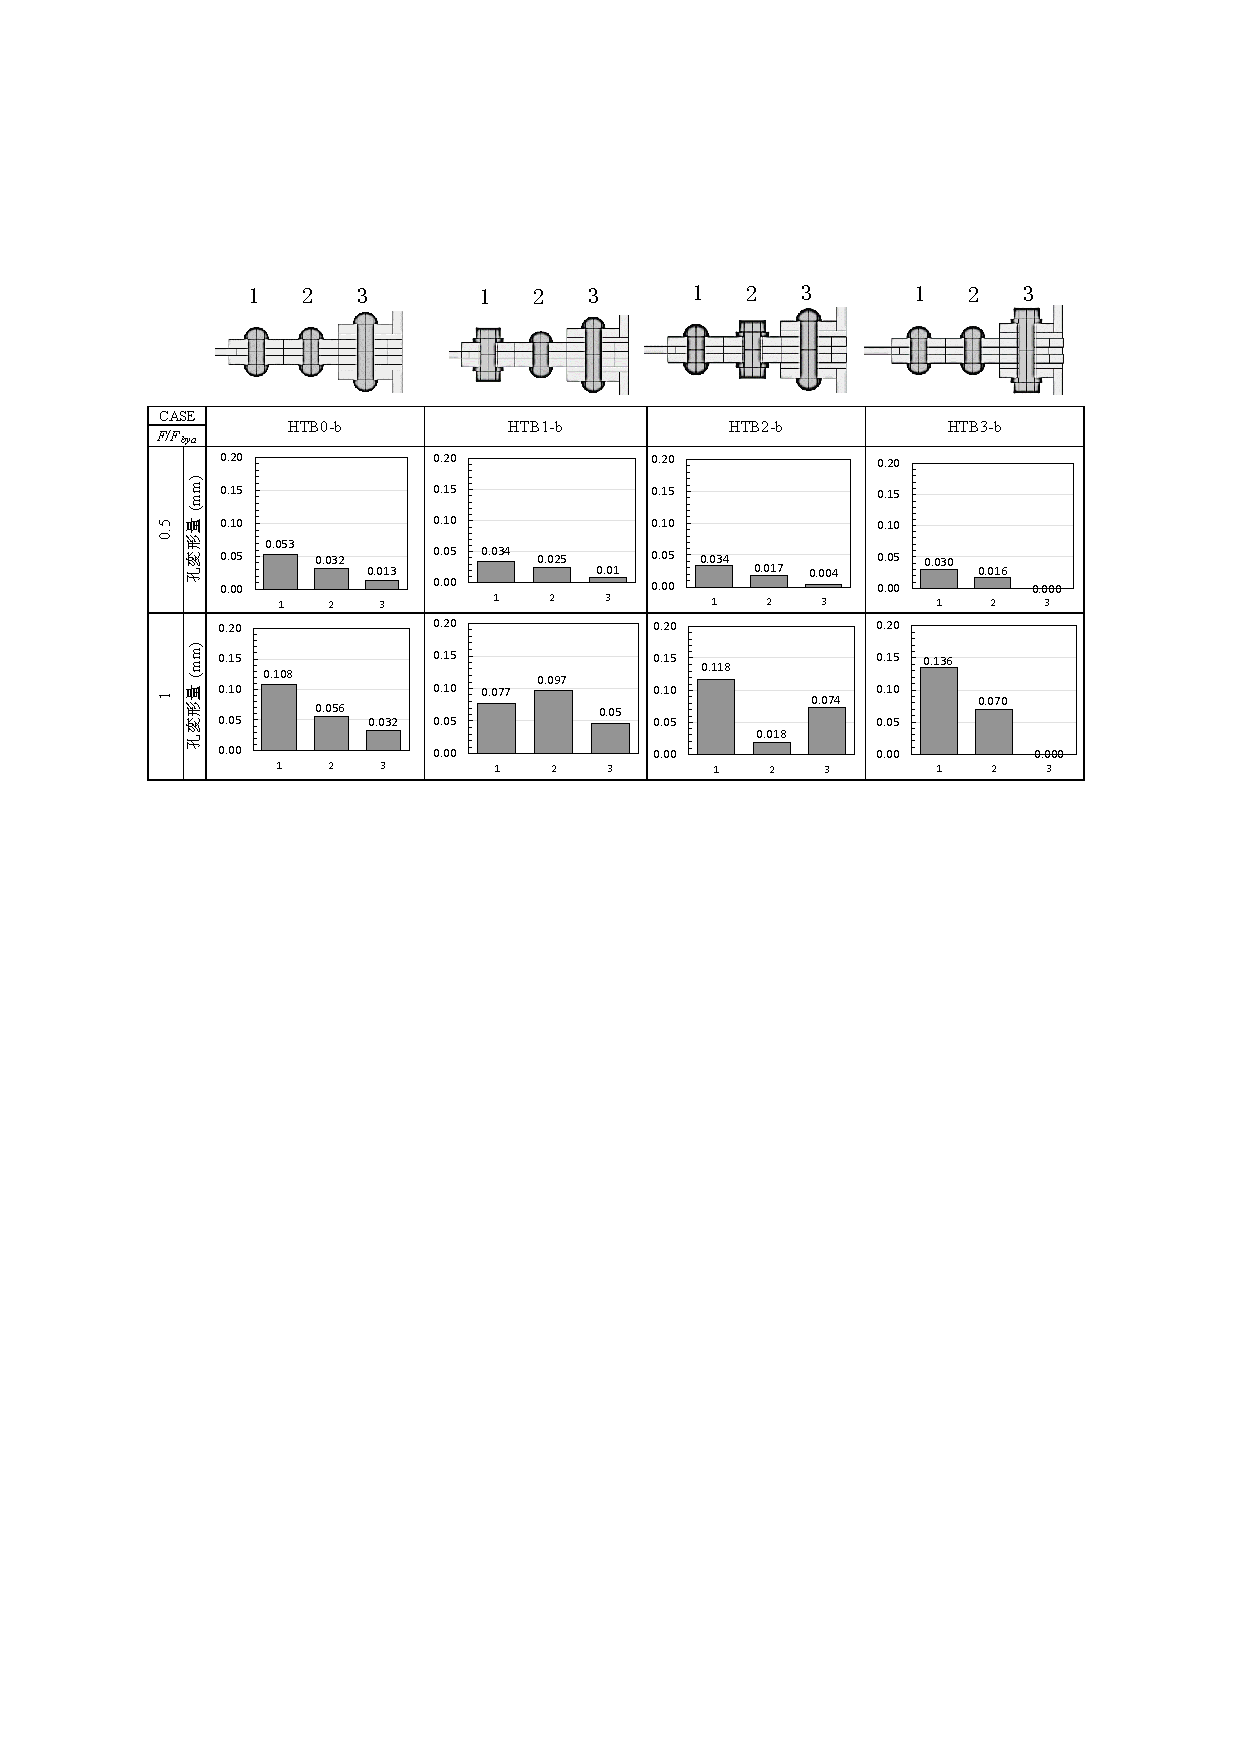
\includegraphics[width=\textwidth]{imgs/ch4/fig19.pdf}
    \caption{Fastener hole deformation $\delta_{hd}$ of each case (bearing yield first type)}
    \label{ch4fig19}
\end{figure}

From Fig. \ref{ch4fig18} and Fig. \ref{ch4fig19}, the hole deformation of each hole is consistent with the relationship between the bearing resistance of each fastener and the amount of deformation of the hole at F / $P_{bya}$  = 1.0 depends on the placement of the rivet and the high-strength bolt, with the most even deformation in the case where the high-strength bolt is placed at fastener position 1.

\begin{figure}[htbp]
    \centering
    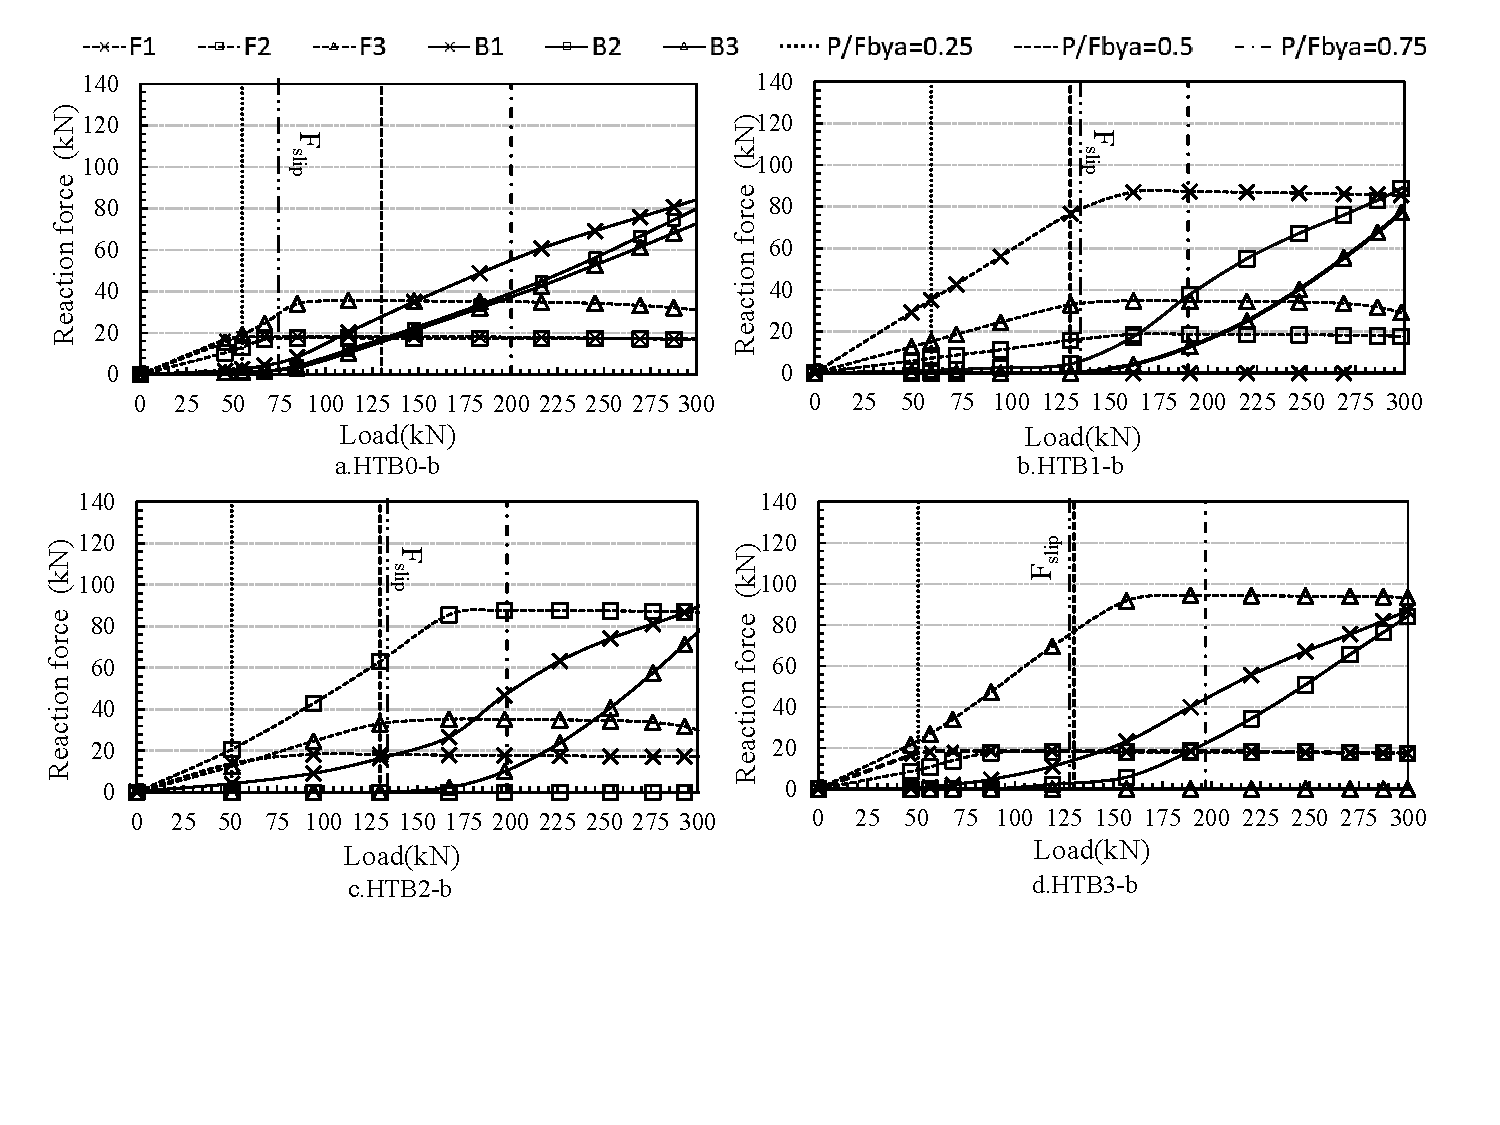
\includegraphics[width=1\linewidth]{imgs//ch4/fast-time-load.pdf}
    \caption{Times change for Friction / Bearing forces and loads of each case}
    \label{fig-fastime}
\end{figure}

Fig. \ref{fig-fastime} shows the relationship between load and friction/support forces. The dotted lines F1 -- F3 represent the frictional forces applied by fasteners 1, 2, and 3, and the solid lines B1~B3 represent the bearing forces applied by fasteners 1, 2, and 3, with X, □, and △ representing fasteners 1 through 3, respectively.

Fig. \ref{fig-fastime} shows that the frictional force due to the rivets did not decrease in any case up to the bearing load, because the bearing deformation of the rivets and the yield deformation of the welded material were slight. On the other hand, after $F / P_{bya}  = 1.25$, the frictional force due to the rivets gradually decreased for HSB1-b and HSB2-b. Therefore, the rivet frictional force can resist the load until the bearing load is reached in the combined use joint.

In the case where a high-strength bolt is placed at fastener position 1 (HSB1-b), the frictional force shared by each fastener increases linearly, there is almost no load sharing by the bearing force before the sliding capacity, and the rigidity of the entire joint is high.

On the other hand, in the HSB0-b, HSB2-b and HSB3-b cases, the slope of the frictional force (F1) due to the rivet at fastener position 1 changed when the load was 50 $kN$ and the frictional force remained constant. This may be due to the fact that the limit value of the rivet friction force is reached at an early stage when a less rigid rivet joint is placed at fastener position 1, where the force acting on the material to be welded is greatest.

\subsubsection{Stress properties of materials to be welded}

\begin{figure}[htbp]
    \centering
    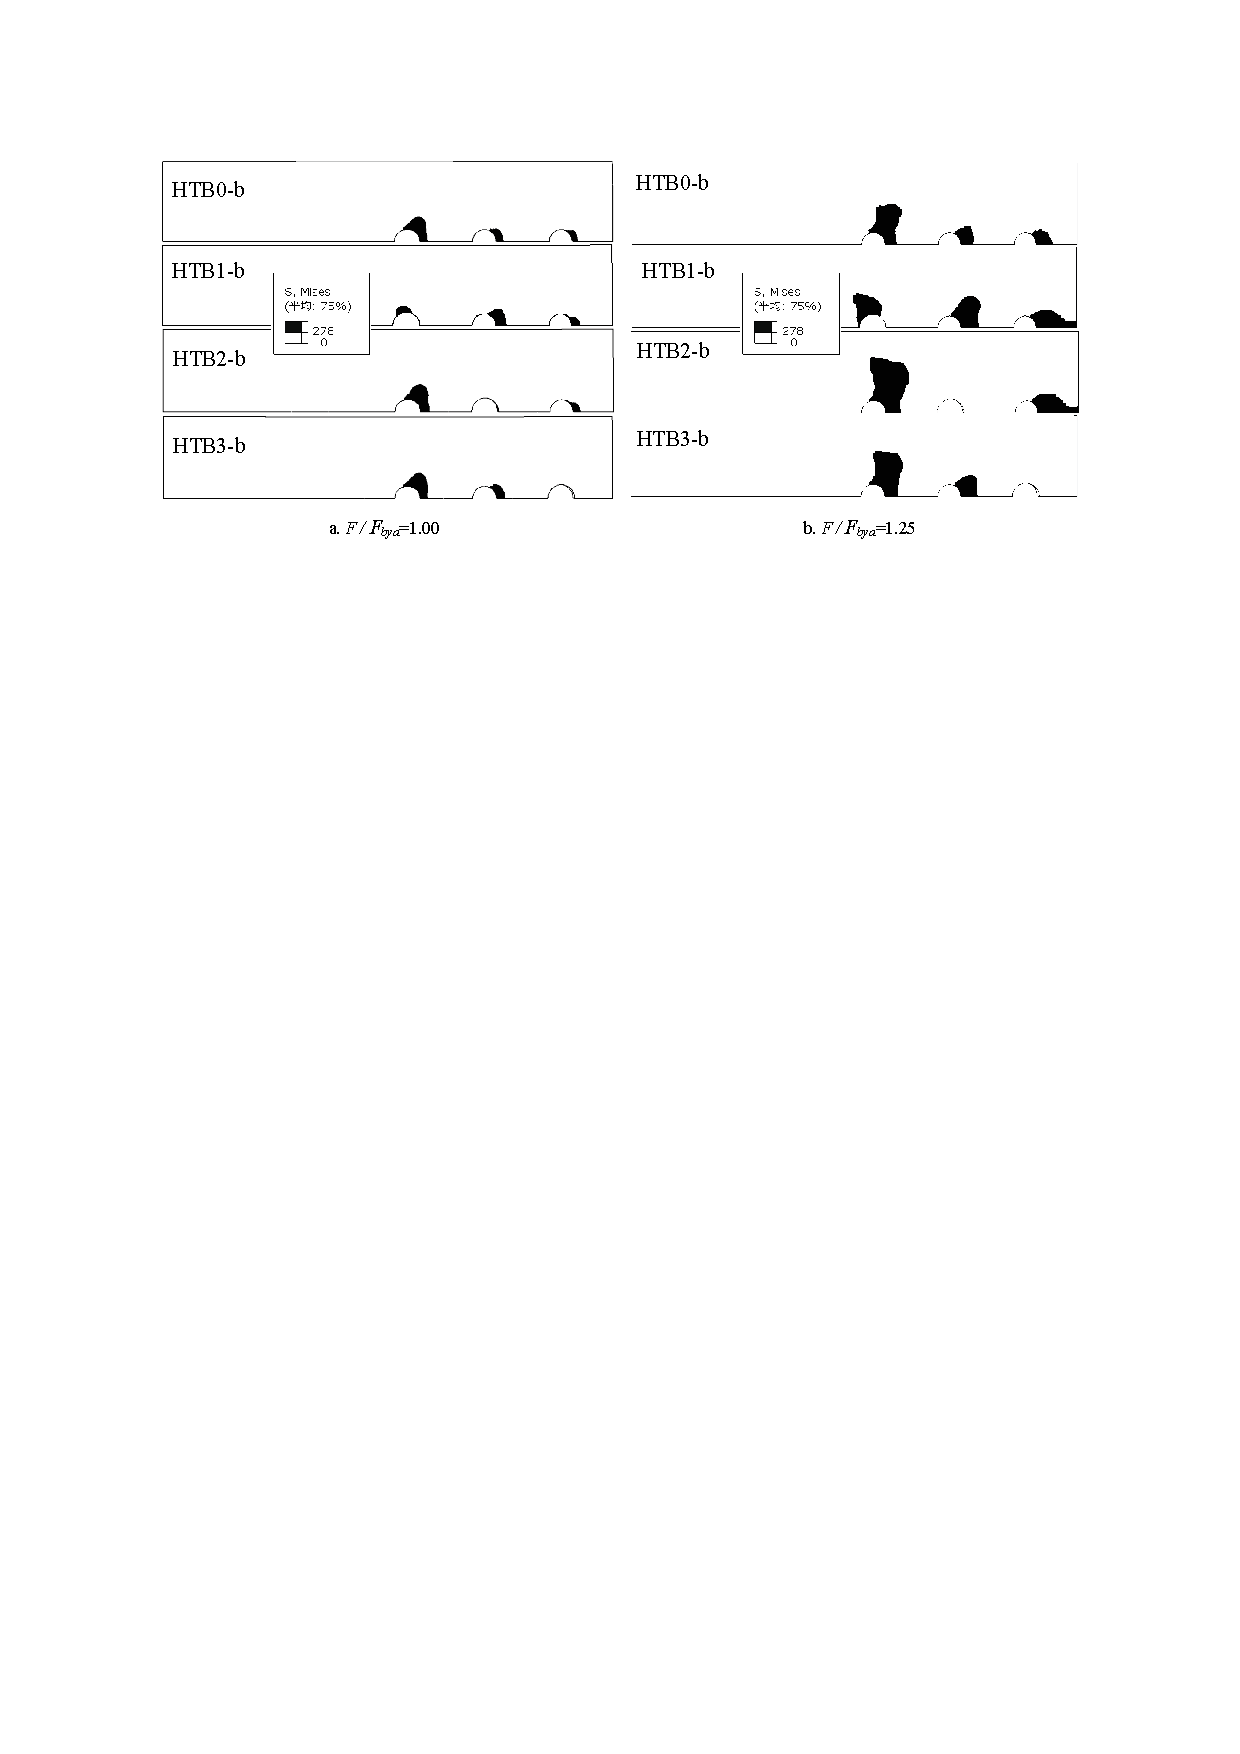
\includegraphics[width=\textwidth]{imgs/ch4/fig21.pdf}
    \caption{plastic area of the main plate (Mises stress $\geq$ yield stress)}
    \label{ch4fig21}
\end{figure}

Fig. \ref{ch4fig21}-a and \ref{ch4fig21}-b show Mises stress contour plots for each case when F / $P_{bya}$  = 1 and 1.25, respectively. Here, black represents the plastic region and white represents the elastic region.

From Fig. \ref{ch4fig21}-a, the plasticization extent of the fastener hole where the high-strength bolt is placed is smaller. Fastener

Table 4 Joint capacity (Unit: $kN$)

\begin{table}
    \caption{Strength of each case (unit: kN)}
    \label{ch4tab4}
    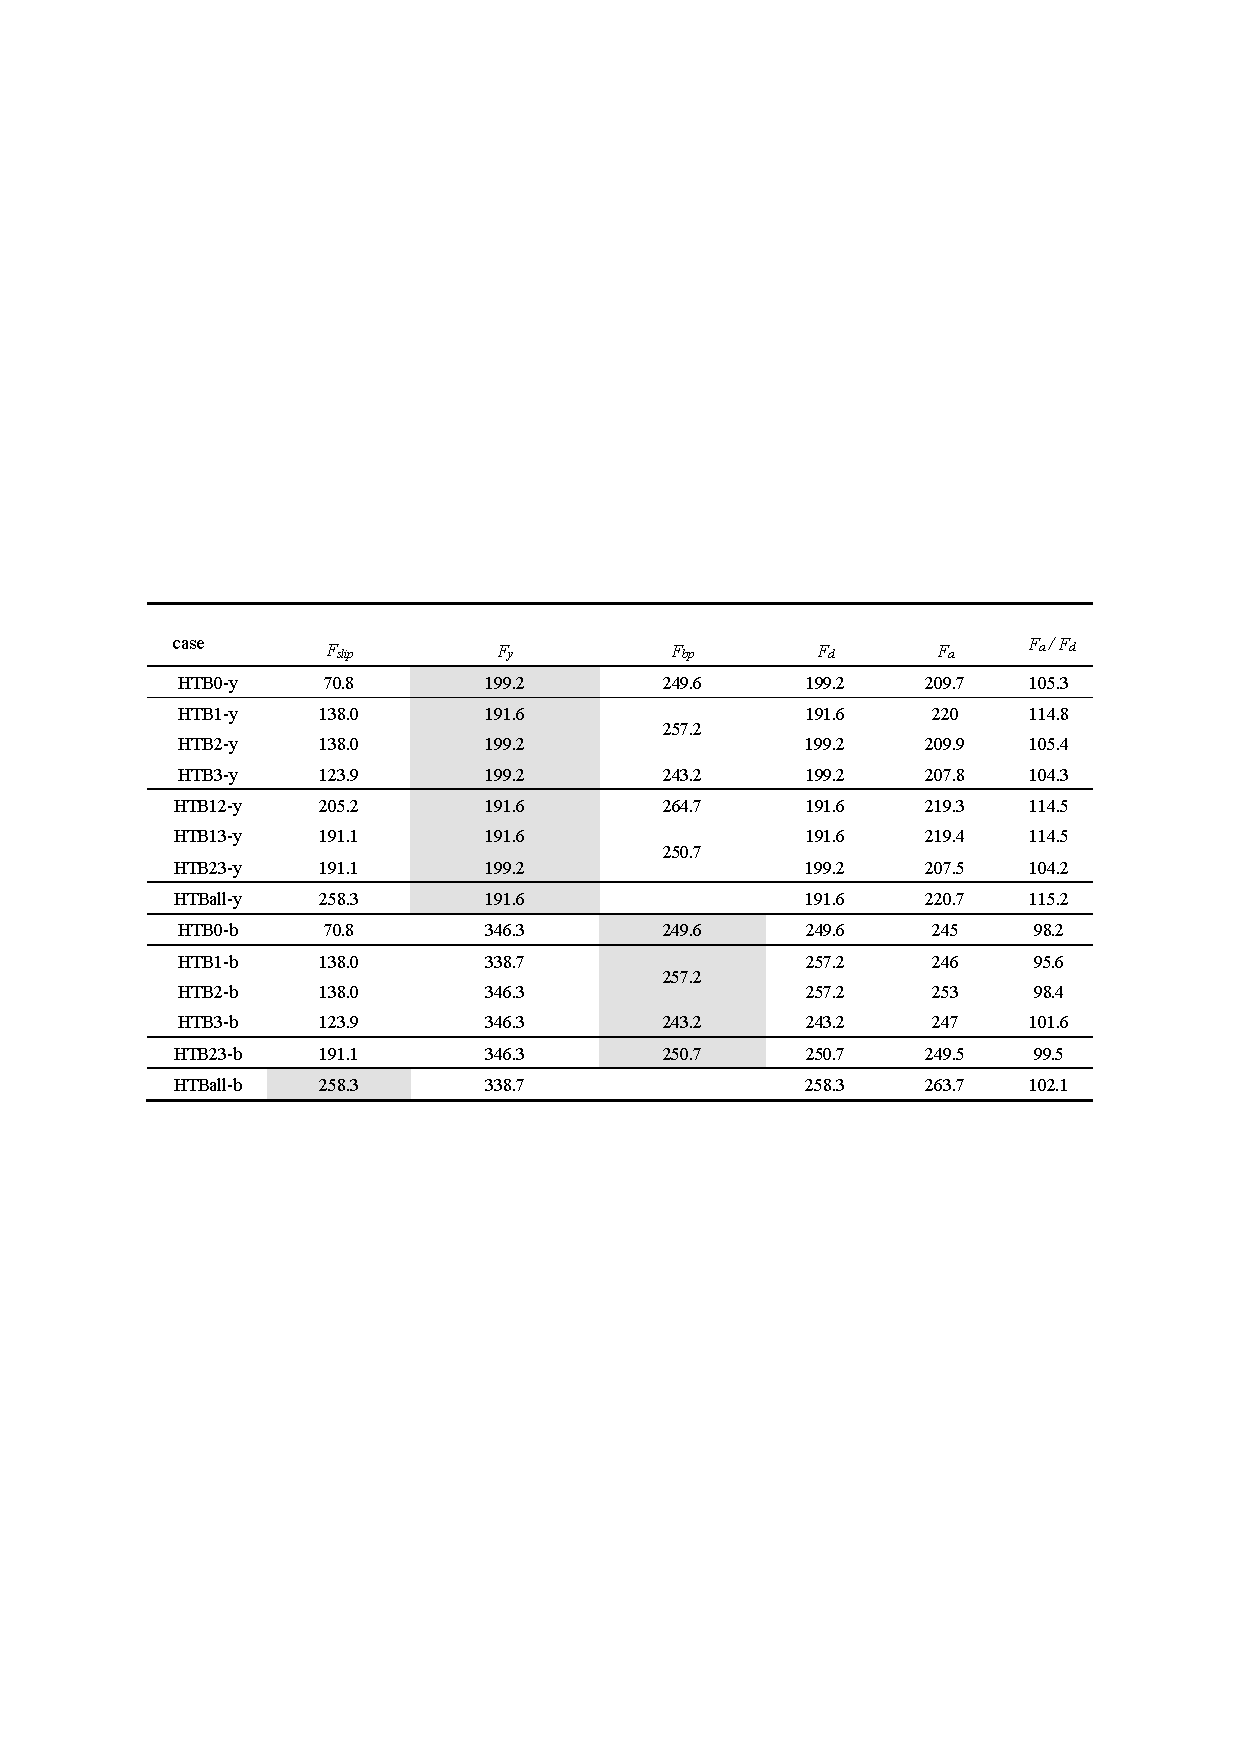
\includegraphics[width=\textwidth]{imgs/ch4/tab4.pdf}
\end{table}

The plasticization extent of fastener position 1 in the HSB2-b and 3-b cases, where no high-strength bolt was placed at position 1, was similar to that of HSB0-b with all rivets. F / $P_{bya}$ = 1 is when the inner rivet holes plasticized in all cases, and the rivet holes plasticized in order from the outside to the inside. That is, nonlinear behavior is not observed until the innermost rivet hole plasticizes. The relationship between the plasticity of each hole and the amount of hole deformation was almost the same at all load levels.

Fig. \ref{ch4fig21}-b shows that when fastener position 3 is a rivet (HSB1-b, HSB2-b), the plastic zone of the innermost rivet hole extended to the edge of the play area. On the other hand, for the HSB3-b case, the plasticity of the innermost rivet hole propagated slower than that of the pure cross-sectional position.
 3.5 Comparison of design capacity and analytical load

Table \ref{ch4tab4} shows the design bearing capacity of the joints, analytical results, and their ratios for each case. The design bearing capacity Fd is the smaller of the net section yield capacity Fy or the improved bearing capacity Fbp .

Table \ref{ch4tab4} shows that for the pure section yield-precedence type, the net section yield load depends on the type of fastener (HSB or rivet) placed at fastener position 1.

For the bearing-precedence type, the difference between the analytical load Fa and the improved bearing capacity Fbp was small, with a maximum difference of 4.4\% and a minimum difference of 0.5\%. In the case of two high-strength bolts, there was no bias in plasticization around the hole due to the support pressure of the rivets, and the difference between the bearing load and the improved bearing capacity was the smallest.


\subsection{Validation of FE Model}

To validate the FEM analysis used in this study, the authors conducted tensile tests on riveted joints cut out of a transverse girder of a riveted bridge that was more than 90 years old. The cut-out positions are shown in Fig. \ref{ch4figA1}.
A total of three cases were set up: friction joint HTBall with all replaced by high-strength bolts, riveted support joint HTB0 and combined joint HTB1 with fastener position 1 as a high-strength bolt.


\begin{figure}[htbp]
    \centering
    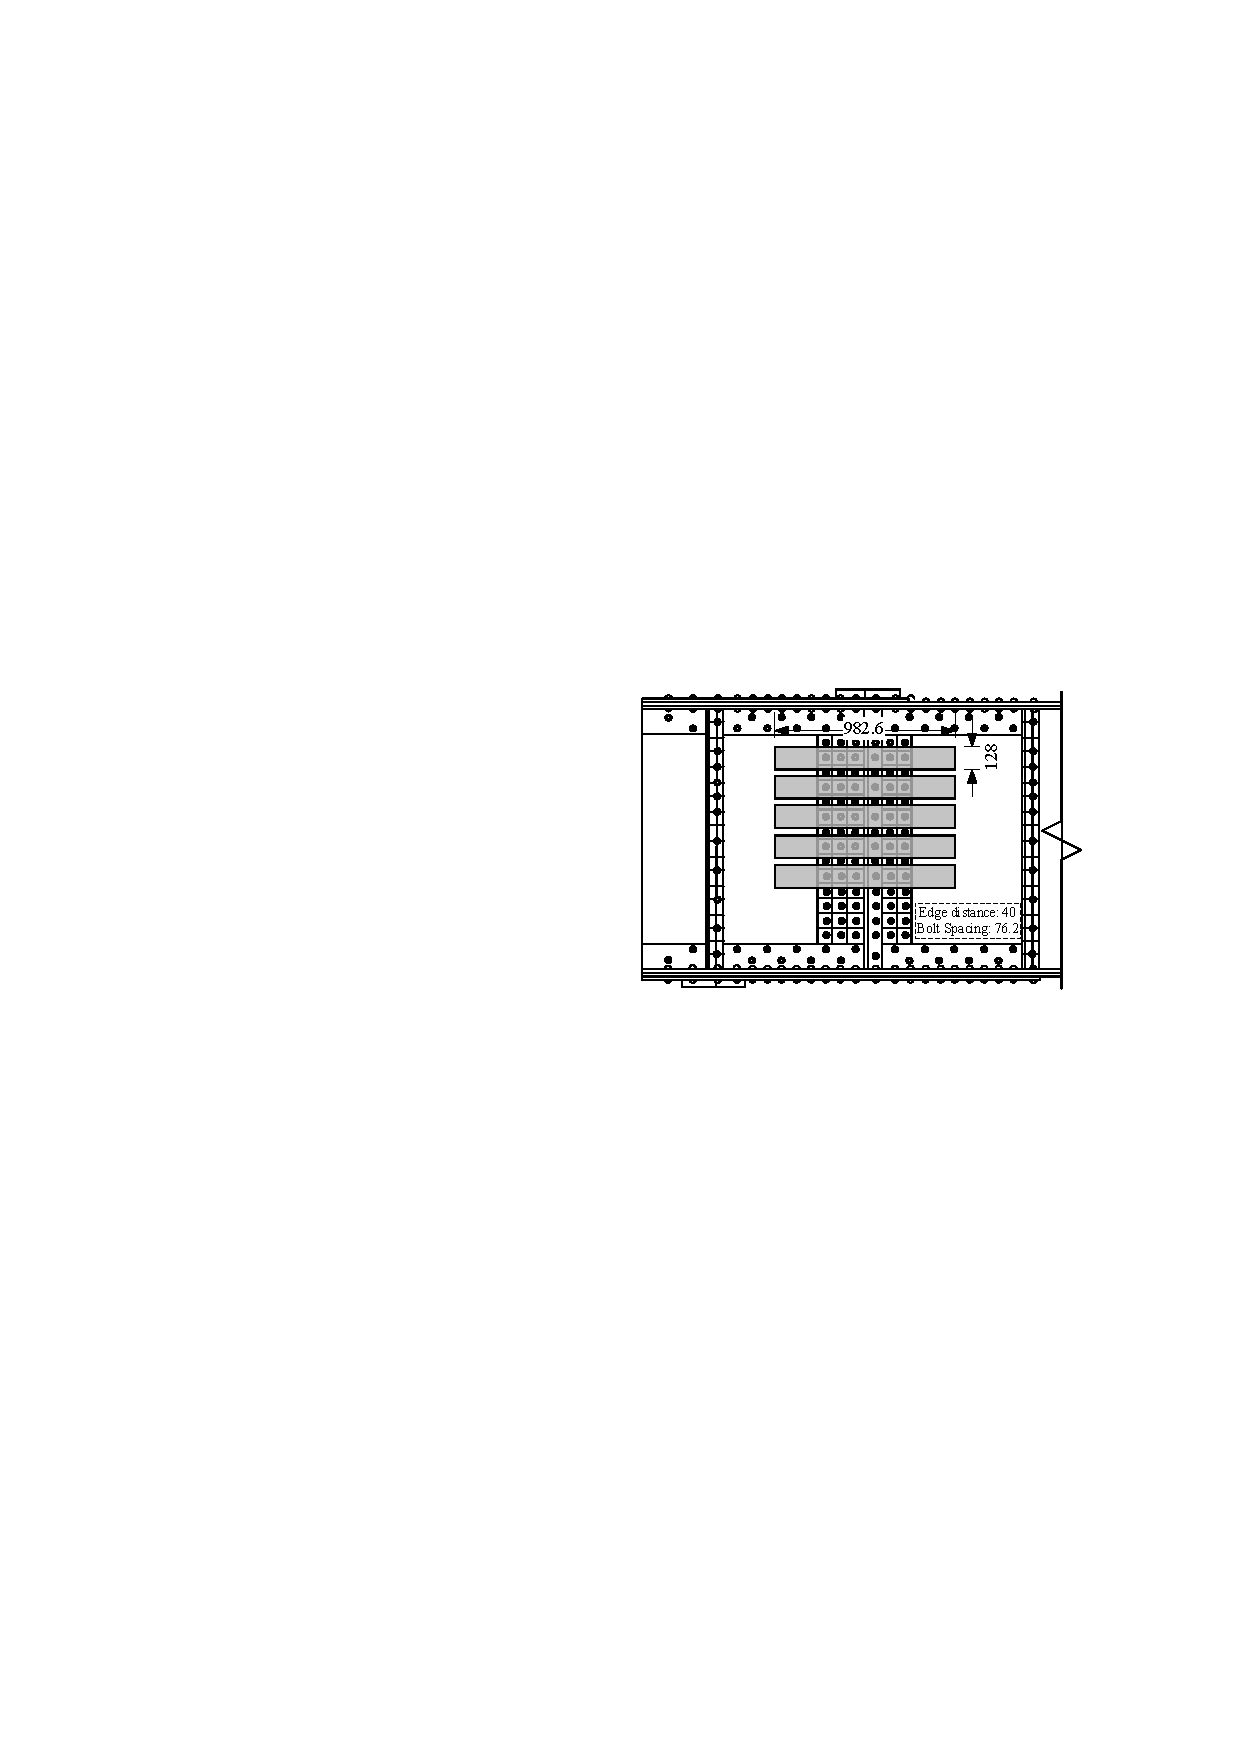
\includegraphics[width=0.6\textwidth]{imgs/ch4/figA1.pdf}
    \caption{Cut out position of riveted joint (unit:mm) }
    \label{ch4figA1}
\end{figure}
 
The dimensions of the analytical model and the introduced axial force of the high-strength bolt were the same as in the experiment. The friction coefficients of the contact surfaces were adjusted so that the sliding loads of the HTBalls matched. The boundary conditions in the analysis were the same as those shown in section \ref{ch4sec2-1}. The installation of the specimen is shown in Fig. \ref{ch4figA2}.

\begin{figure}[htbp]
    \centering
    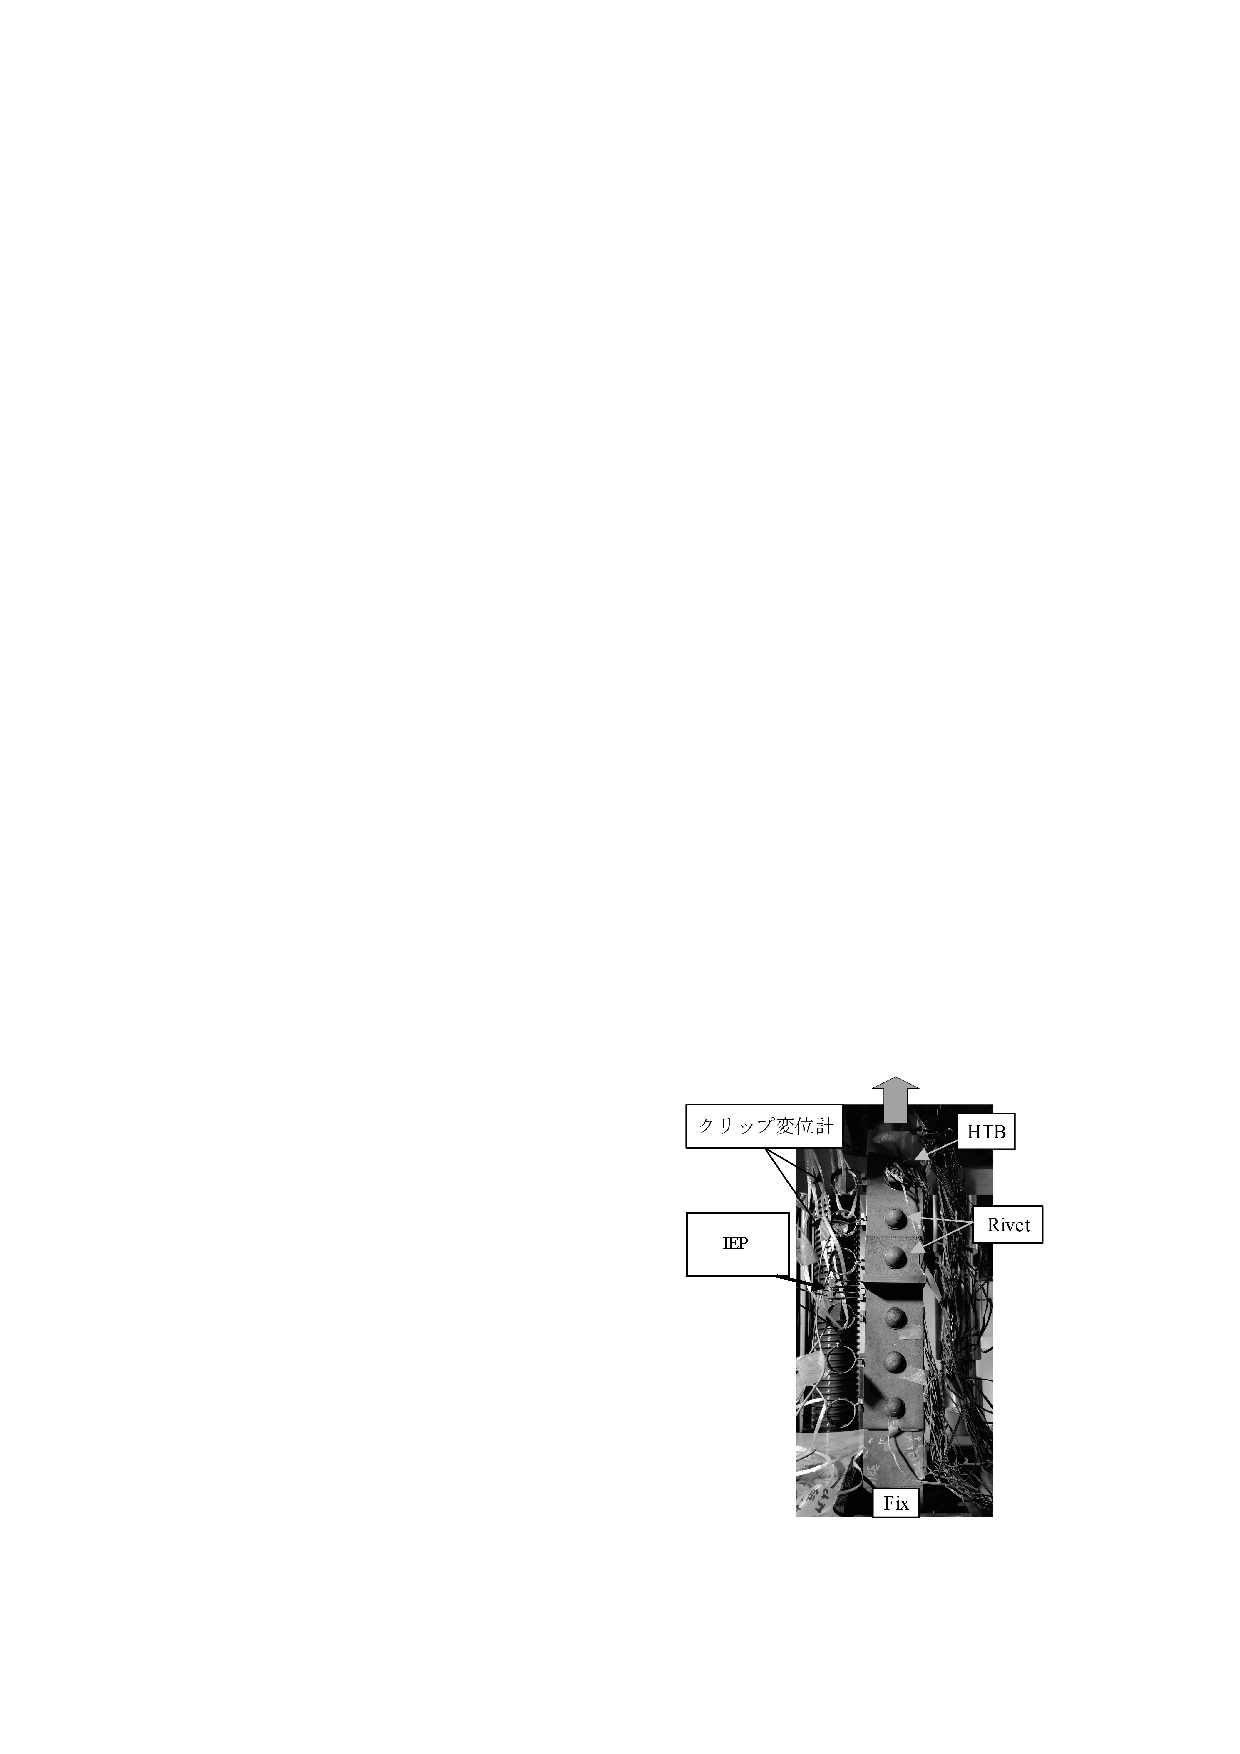
\includegraphics[width=0.5\textwidth]{imgs/ch4/figA2.pdf}
    \caption{Set-up for HTB1 case}
    \label{ch4figA2}
\end{figure}

\subsubsection{Comparison of experimental and analytical results}

The load and relative displacement relationships for HTBall, HTB0 and HTB1 are shown in Fig. \ref{ch4figA3}. The relative displacement between the contact plate and the welded material was measured at a position 10 mm from the gap in both the analysis and the experiment.
Fig. \ref{ch4figA3} shows that the curves of the load-relative displacement relationship for the riveted HTB0 joints from the experiments and the analysis are almost identical. In HTB1, the initial stiffnesses of the two joints are almost identical up to a value of F / Fy = 0.8. However, there is a difference between the two after that point. This is thought to be due to the fact that in the experiment the slip capacity was exceeded, which resulted in minute slippage.

\begin{figure}[htbp]
    \centering
    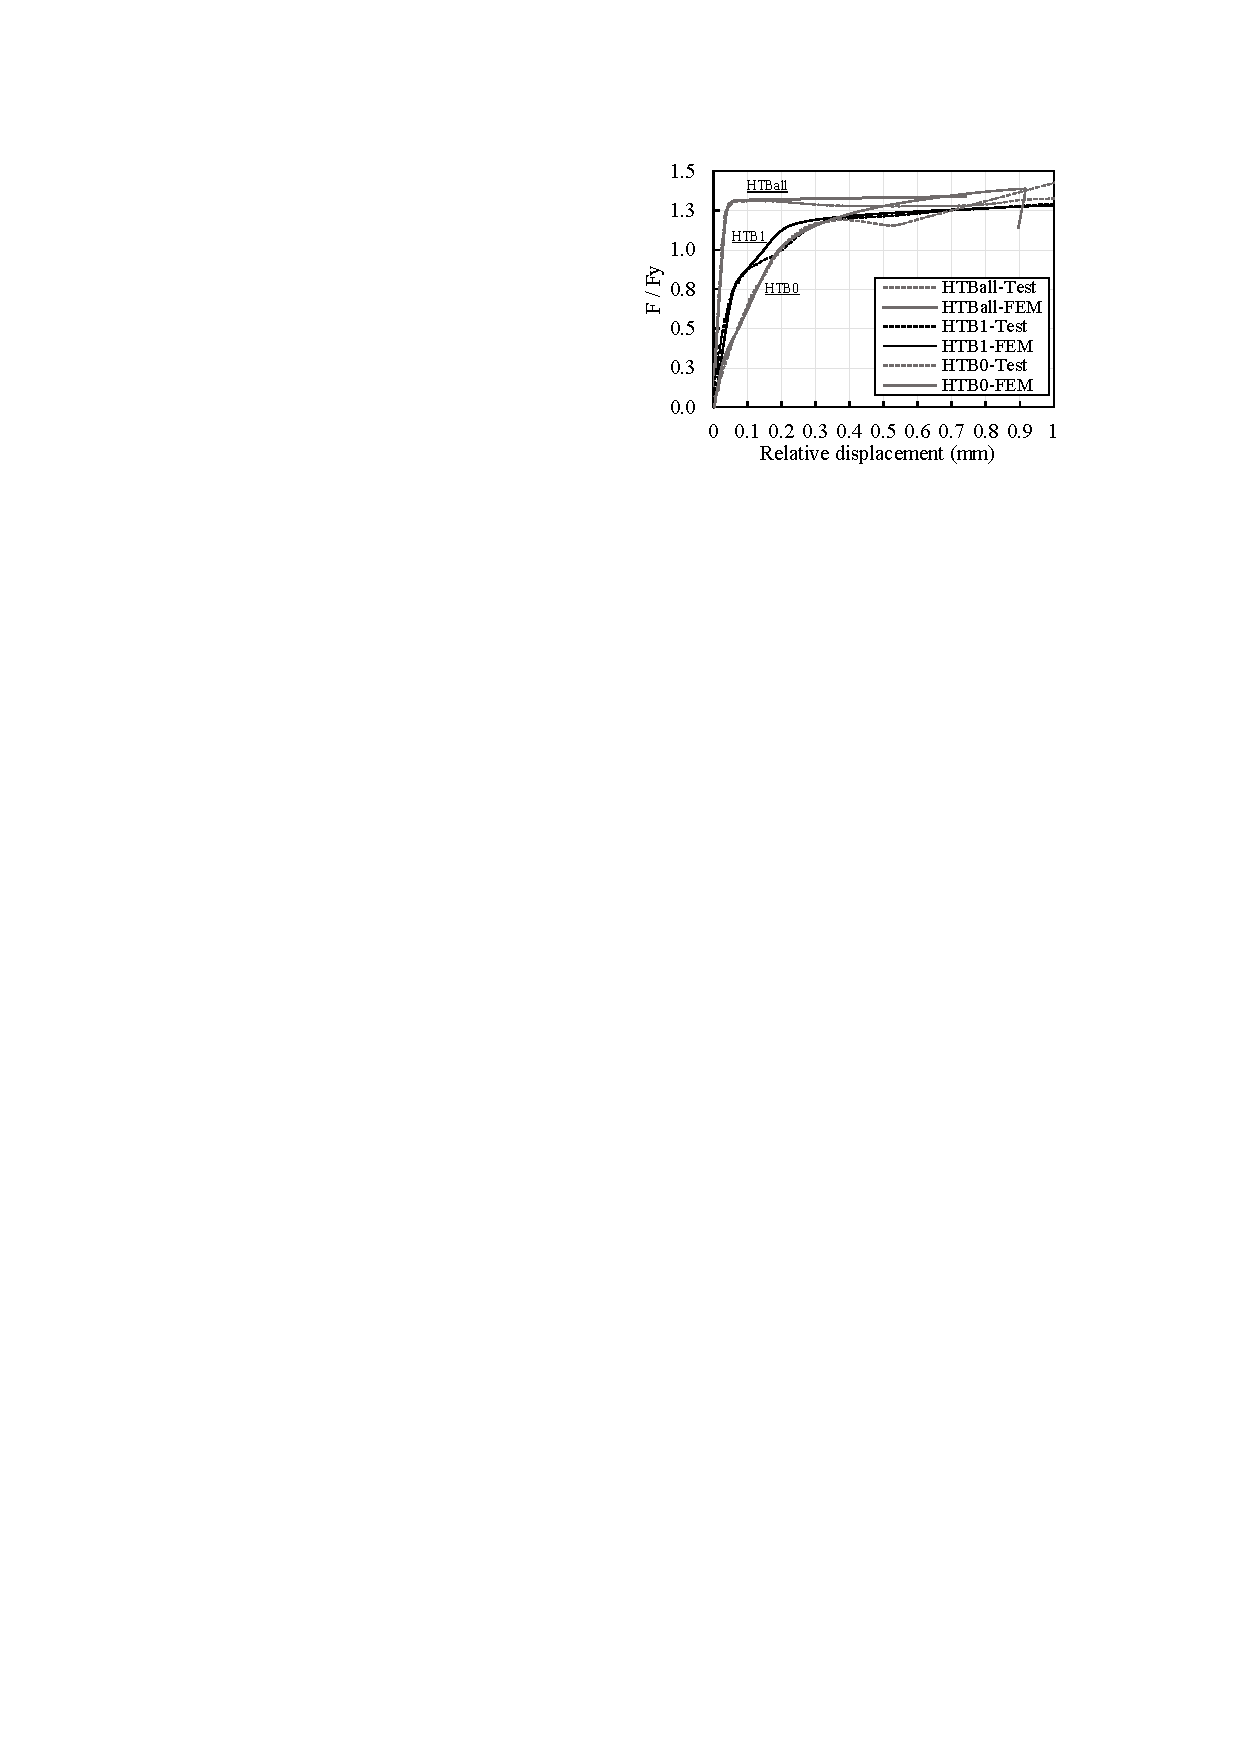
\includegraphics[width=0.7\textwidth]{imgs/ch4/figA3.pdf}
    \caption{Relationship between load and replative displacement (compair experiment and FE analysis result)}
    \label{ch4figA3}
\end{figure}

\subsubsection{Strain distribution in the joints}

The strain distributions in the tensile direction on the kovar surface of the jointed material in the HTB0 and HTB1 cases are shown in Fig. \ref{ch4figA4} a and b respectively $(F / F_y = 0.6 and 1.0)$. The strain measurement positions are shown in Fig. \ref{ch4figA5}.
Fig. \ref{ch4figA4} a and b show that the experimental and analytical strain distributions on the cobber surface of the jointed material at $F / F_y = 0.6$ are in good agreement for both HTB0 and HTB1.
The experimental and analytical strain distributions at $F / F_y = 1$ showed a similar trend for both HTB0 and HTB1. However, the analytical results for HTB0 were smaller than the experimental results at ε1 to ε5. This may be because the actual secondary stiffness is smaller than $E/100$, although the material constitutive law in the analysis is a bilinear law with a secondary stiffness of$ E/100$ (E=200,000 MPa).

\begin{figure}[htbp]
    \centering
    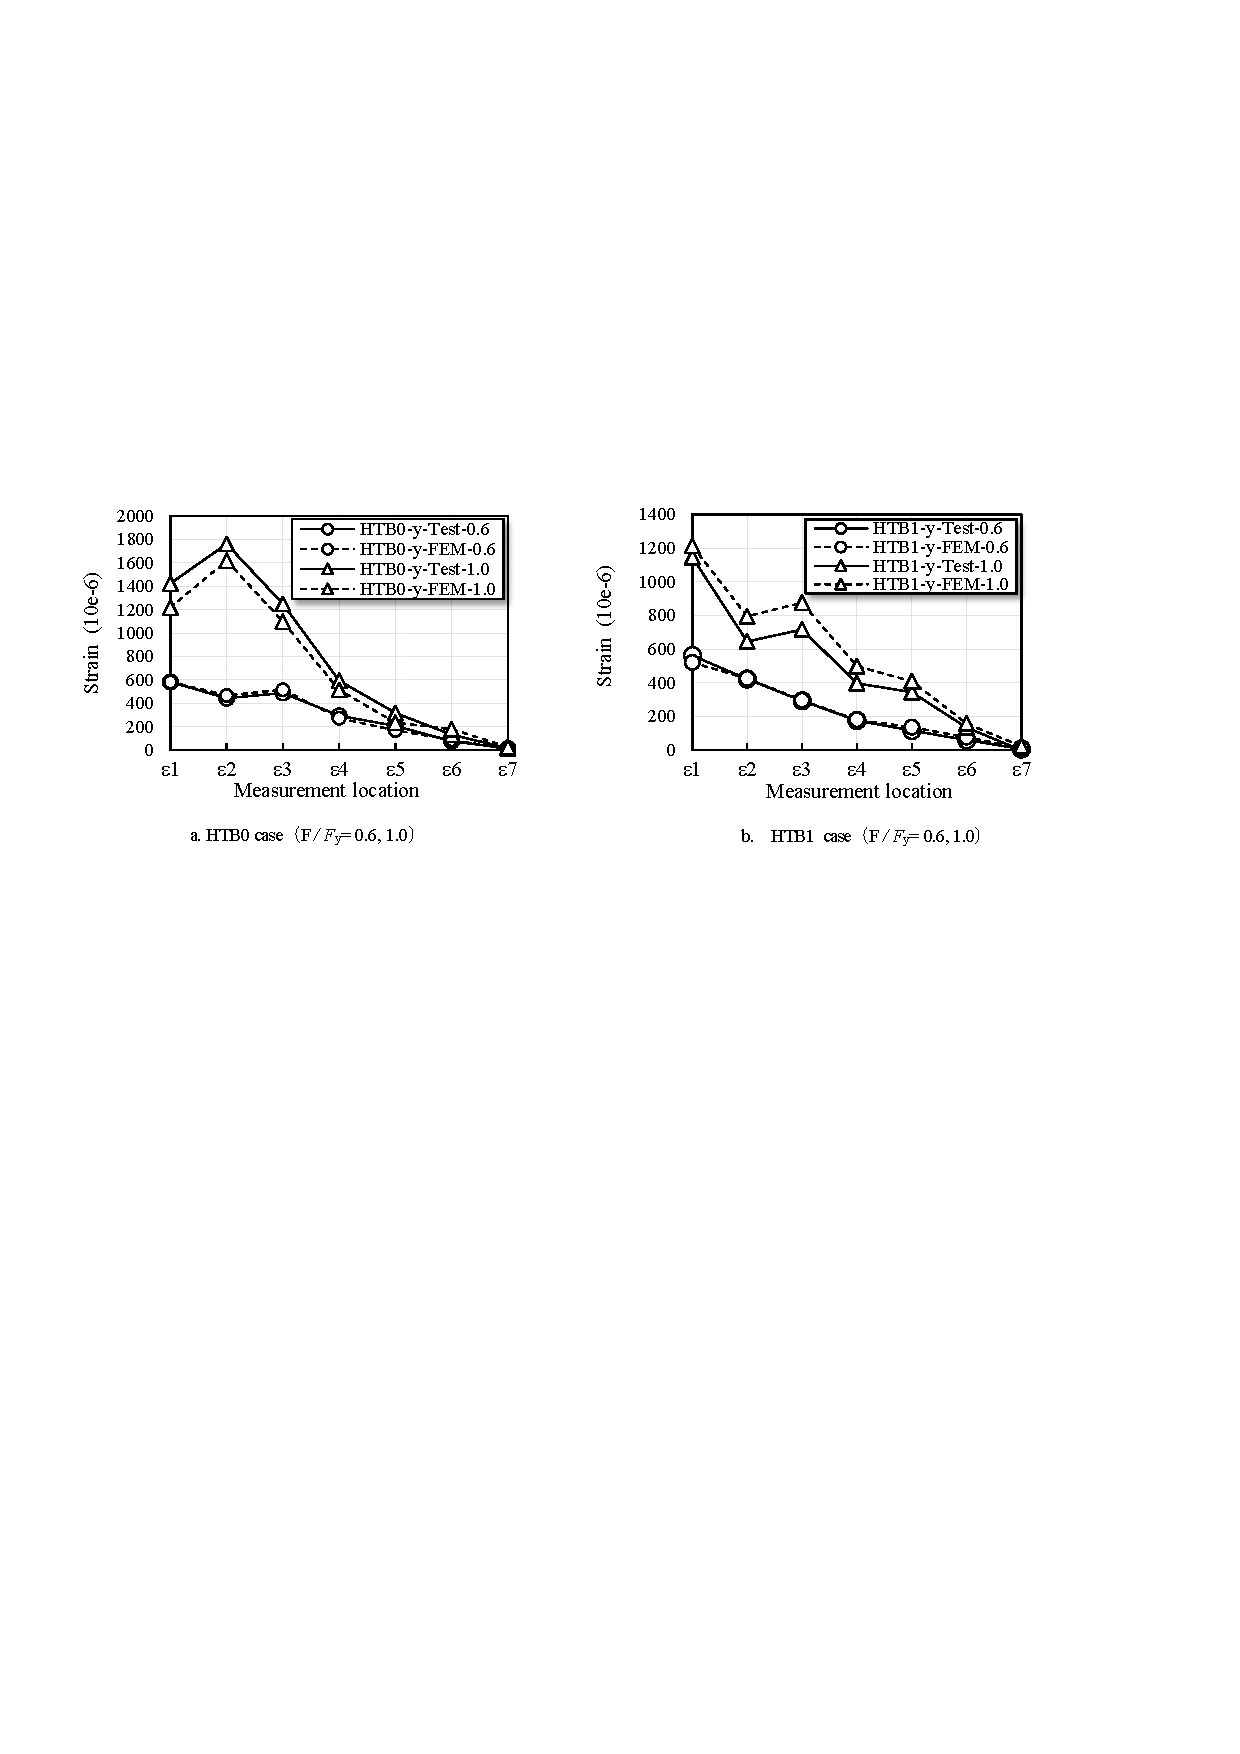
\includegraphics[width=\textwidth]{imgs/ch4/figA4.pdf}
    \caption{Strain distribution of main plate}
    \label{ch4figA4}
\end{figure}

\begin{figure}[htbp]
    \centering
    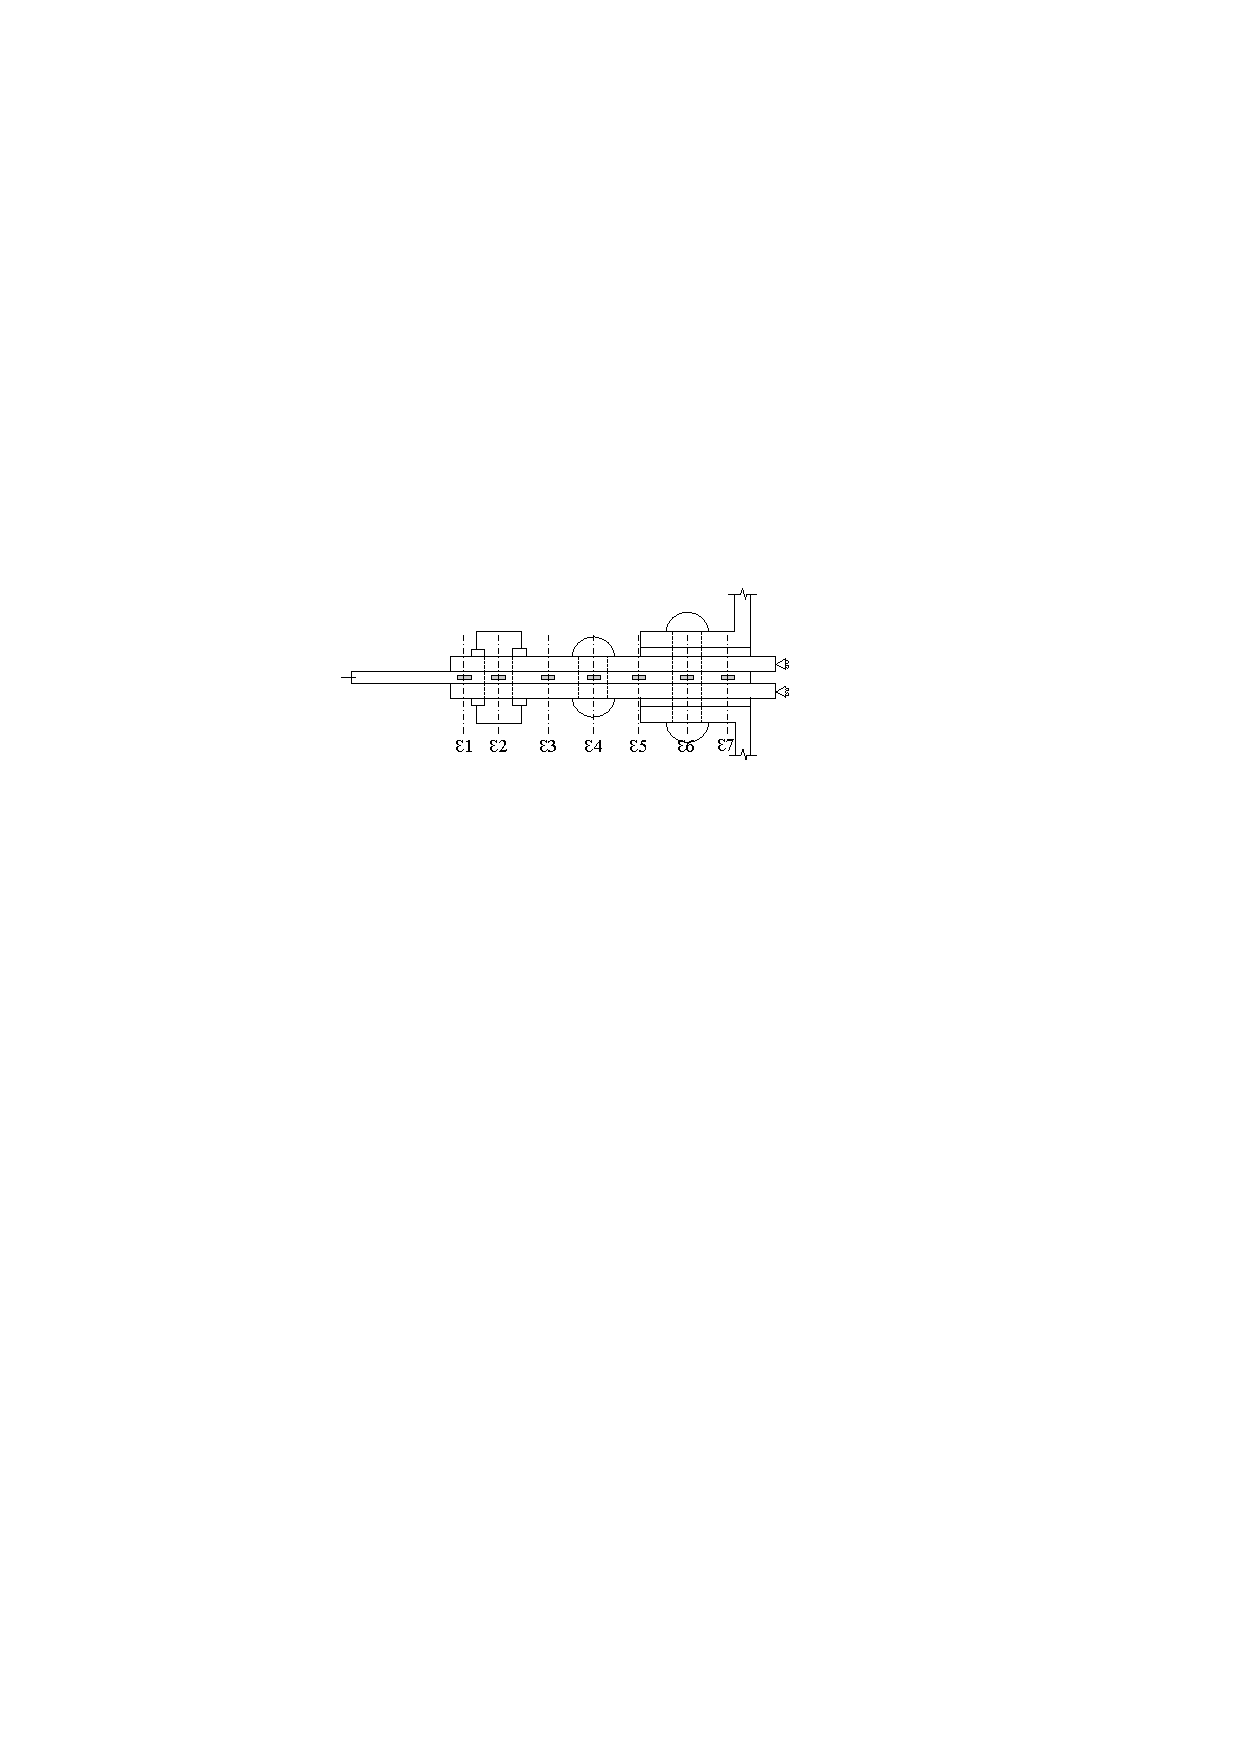
\includegraphics[width=0.75\textwidth]{imgs/ch4/figA5.pdf}
    \caption{Measuring position for the strain}
    \label{ch4figA5}
\end{figure}

\subsubsection{Residual axial forces of the bolt}

Fig. \ref{ch4figA6} and Fig. \ref{ch4figA7} show the relationship between experimental and analytical loads and bolt axial force survivability (bolt axial force/initial bolt axial force) for HTBall and HTB1 respectively. The axial force remaining ratio is the ratio of the bolt axial force to the pre-test value; HTB0 is excluded from the comparison because the rivet axial force could not be ascertained in the experiment.
From Appendix Figs. 6 and 7, the changes in the remaining bolt axial force between the experiment and the analysis are in good agreement.

\begin{figure}[htbp]
    \centering
    \begin{minipage}[t]{0.48\textwidth}
    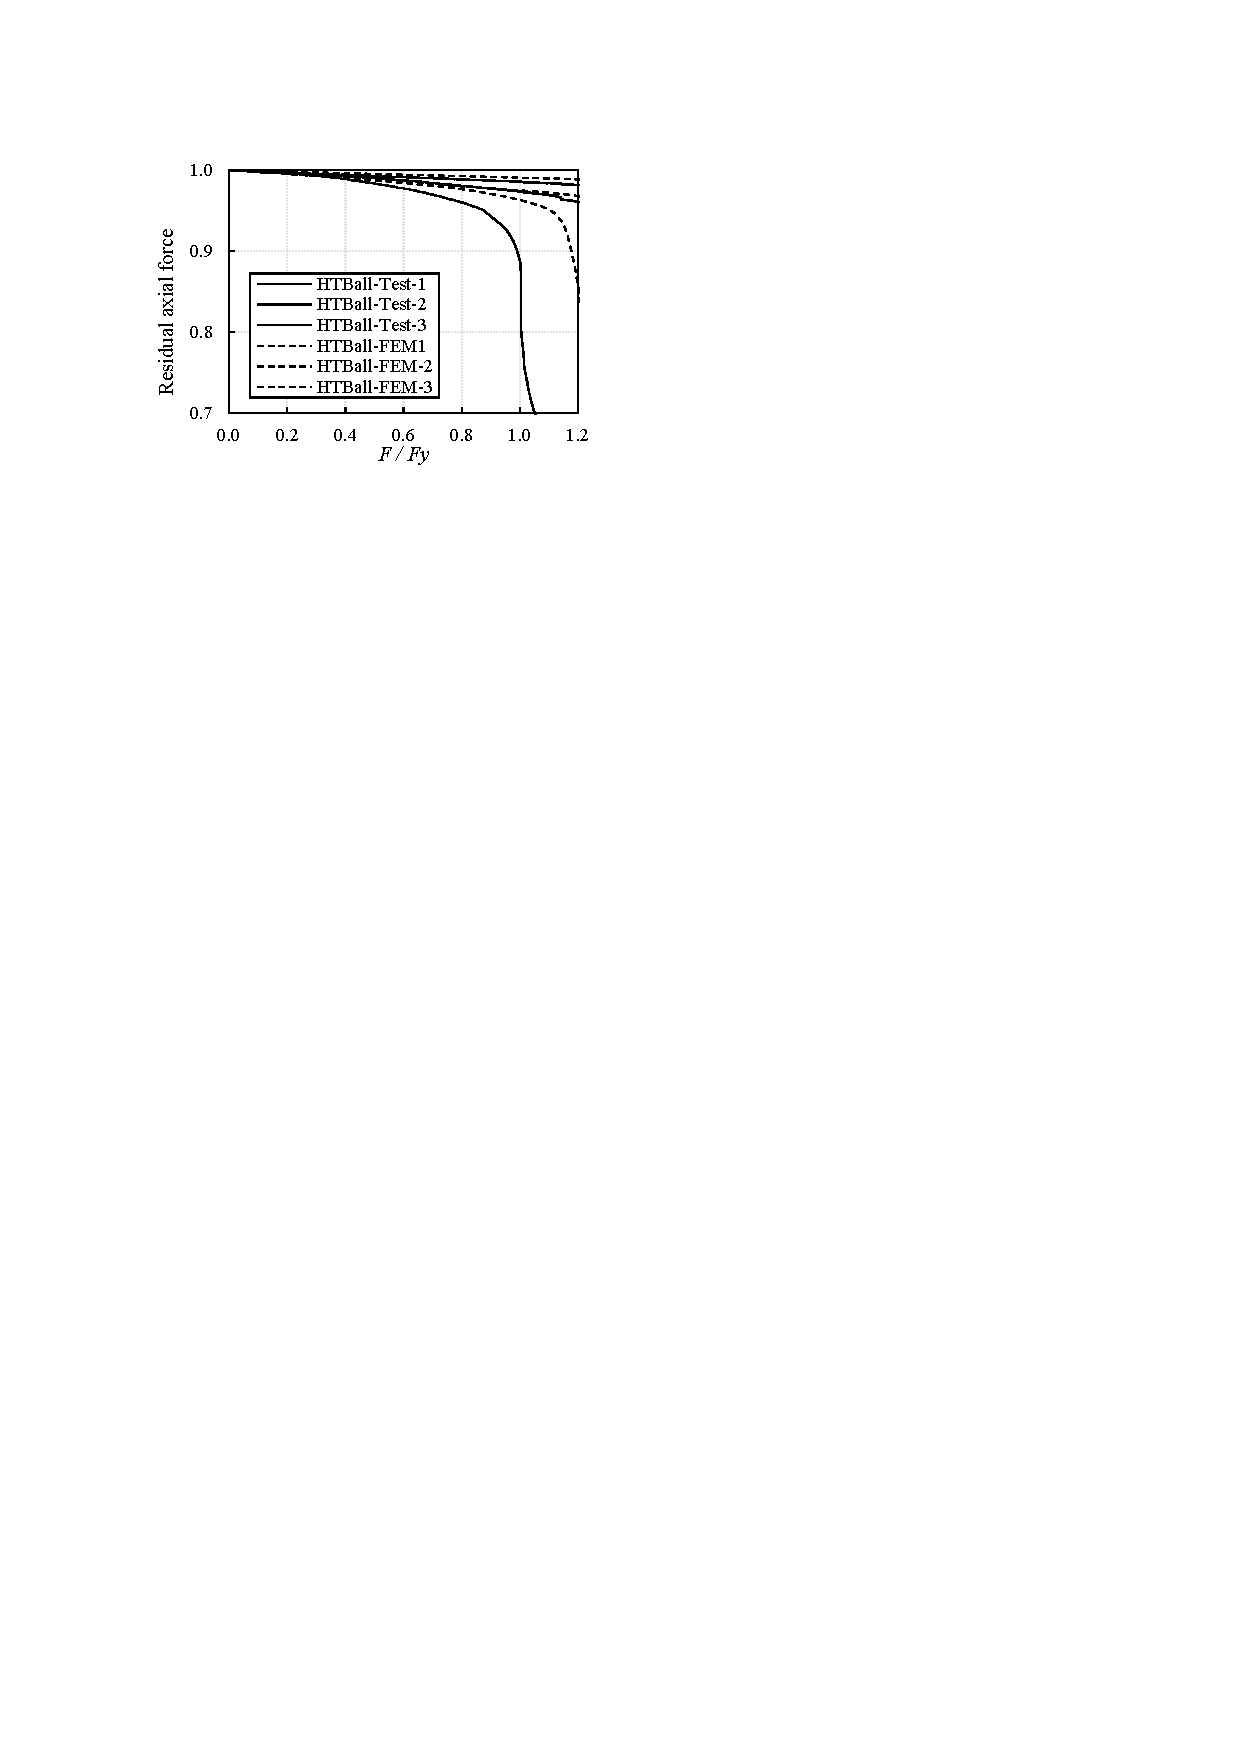
\includegraphics[width=\linewidth]{imgs/ch4/figA6.pdf}
    \caption{Changing of residual axial force of HTBall case}
    \label{ch4figA6}
    \end{minipage}
    \begin{minipage}[t]{0.48\textwidth}
    \centering
    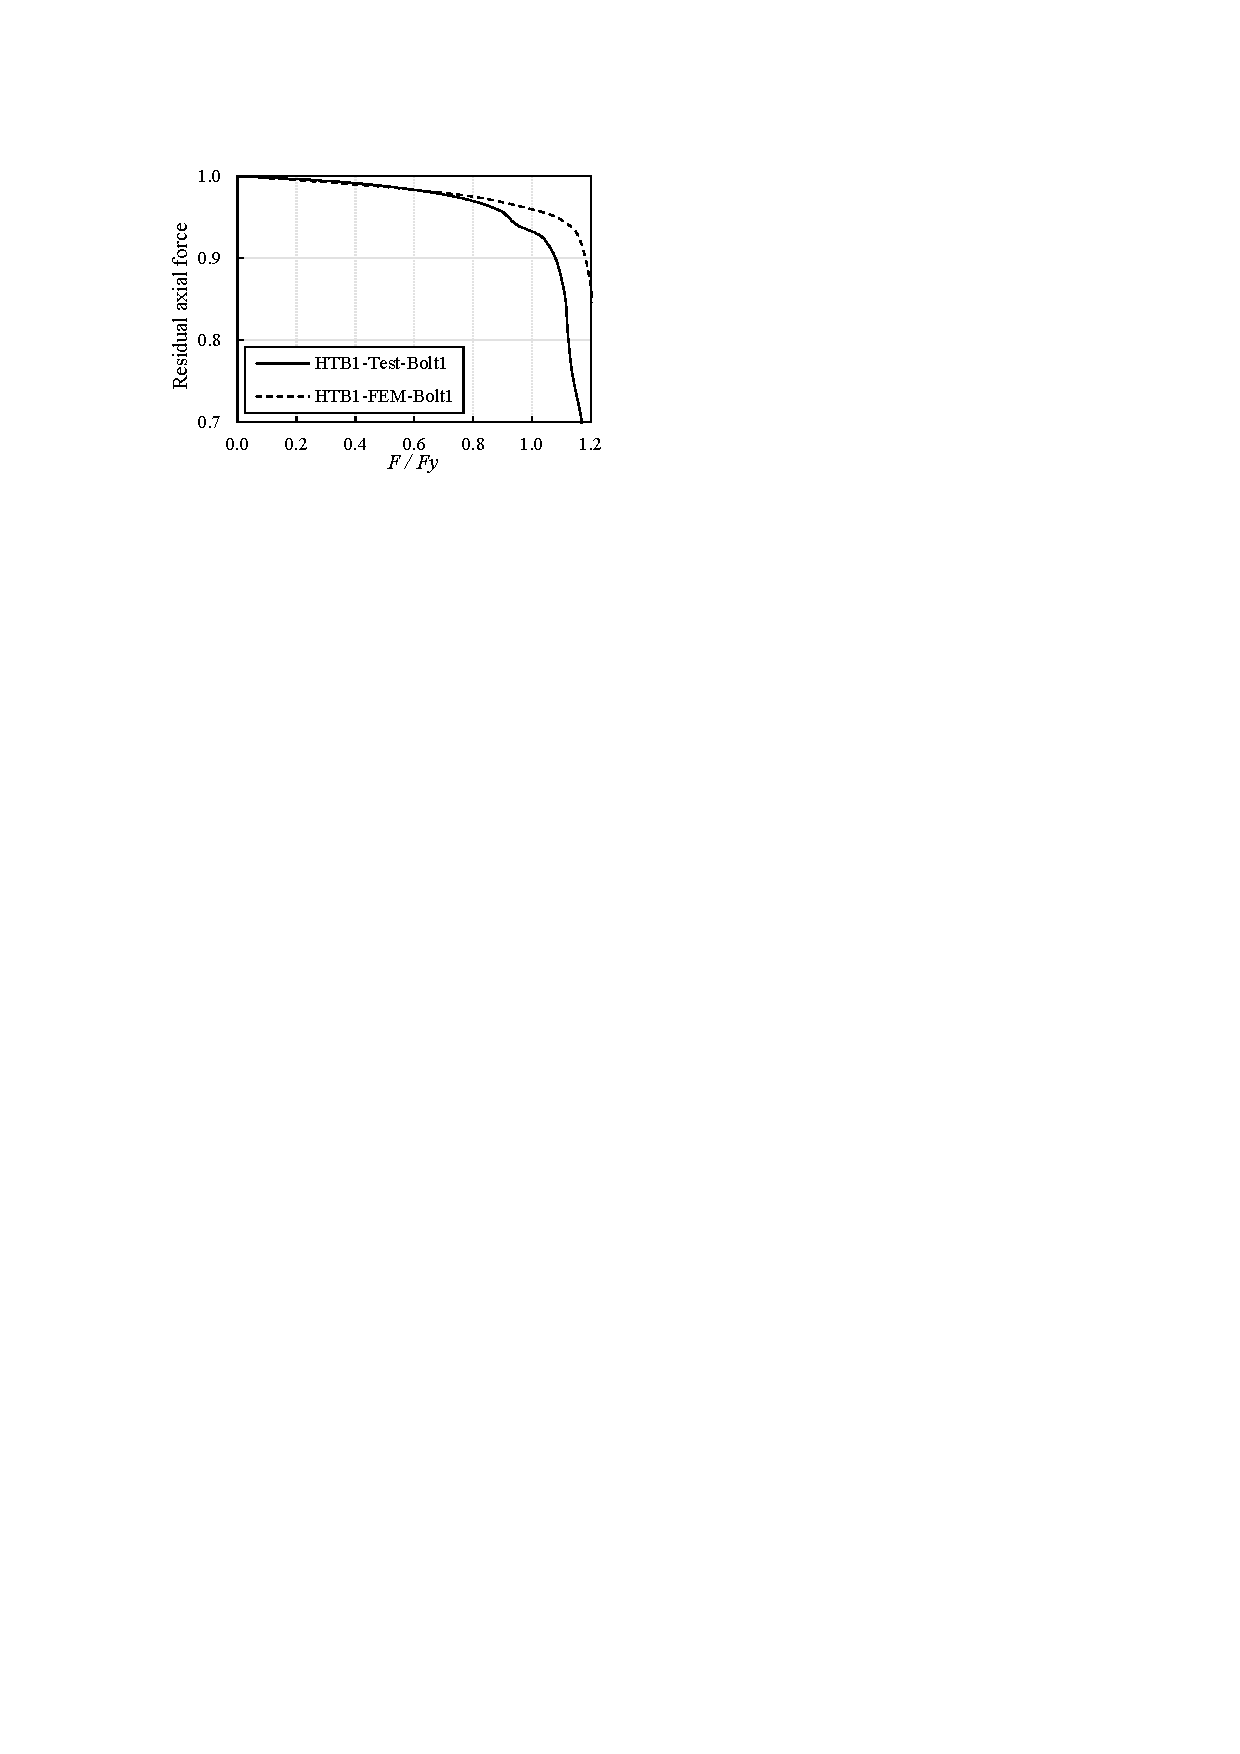
\includegraphics[width=\linewidth]{imgs/ch4/figA7.pdf}
    \caption{Changing of residual axial force of HTB1 case}
    \label{ch4figA7}
    \end{minipage}
\end{figure}

\subsubsection{Validation results}

The load-relative displacement relationship and bolt axial force remaining ratio between the experimental and analytical results using the analytical model and method presented here are in good agreement. On the other hand, the strain distribution in the jointed material was in perfect agreement for$ F / F_y = 0.6$, but for $F / F_y = 1$ there was a slight deviation from the experimental data. However, the deviations were within 10%.
In conclusion, it is considered possible to analytically evaluate the mechanical behaviour of combined joints with rivets and high-strength bolts using the analytical model and methods used in this study.


\section{Investigate the Replacement of The Bolt}

The model was developed in Abaqus, and the FE mesh and boundary conditions imposed are shown in Fig. \ref{fig-l5}. To simulate the dead load, distributed loads were applied to the joint end surface. The elements applied in the model were three-dimensional eight node solid elements with reduced integration (C3D8R).

\begin{figure}[htbp]
    \centering
    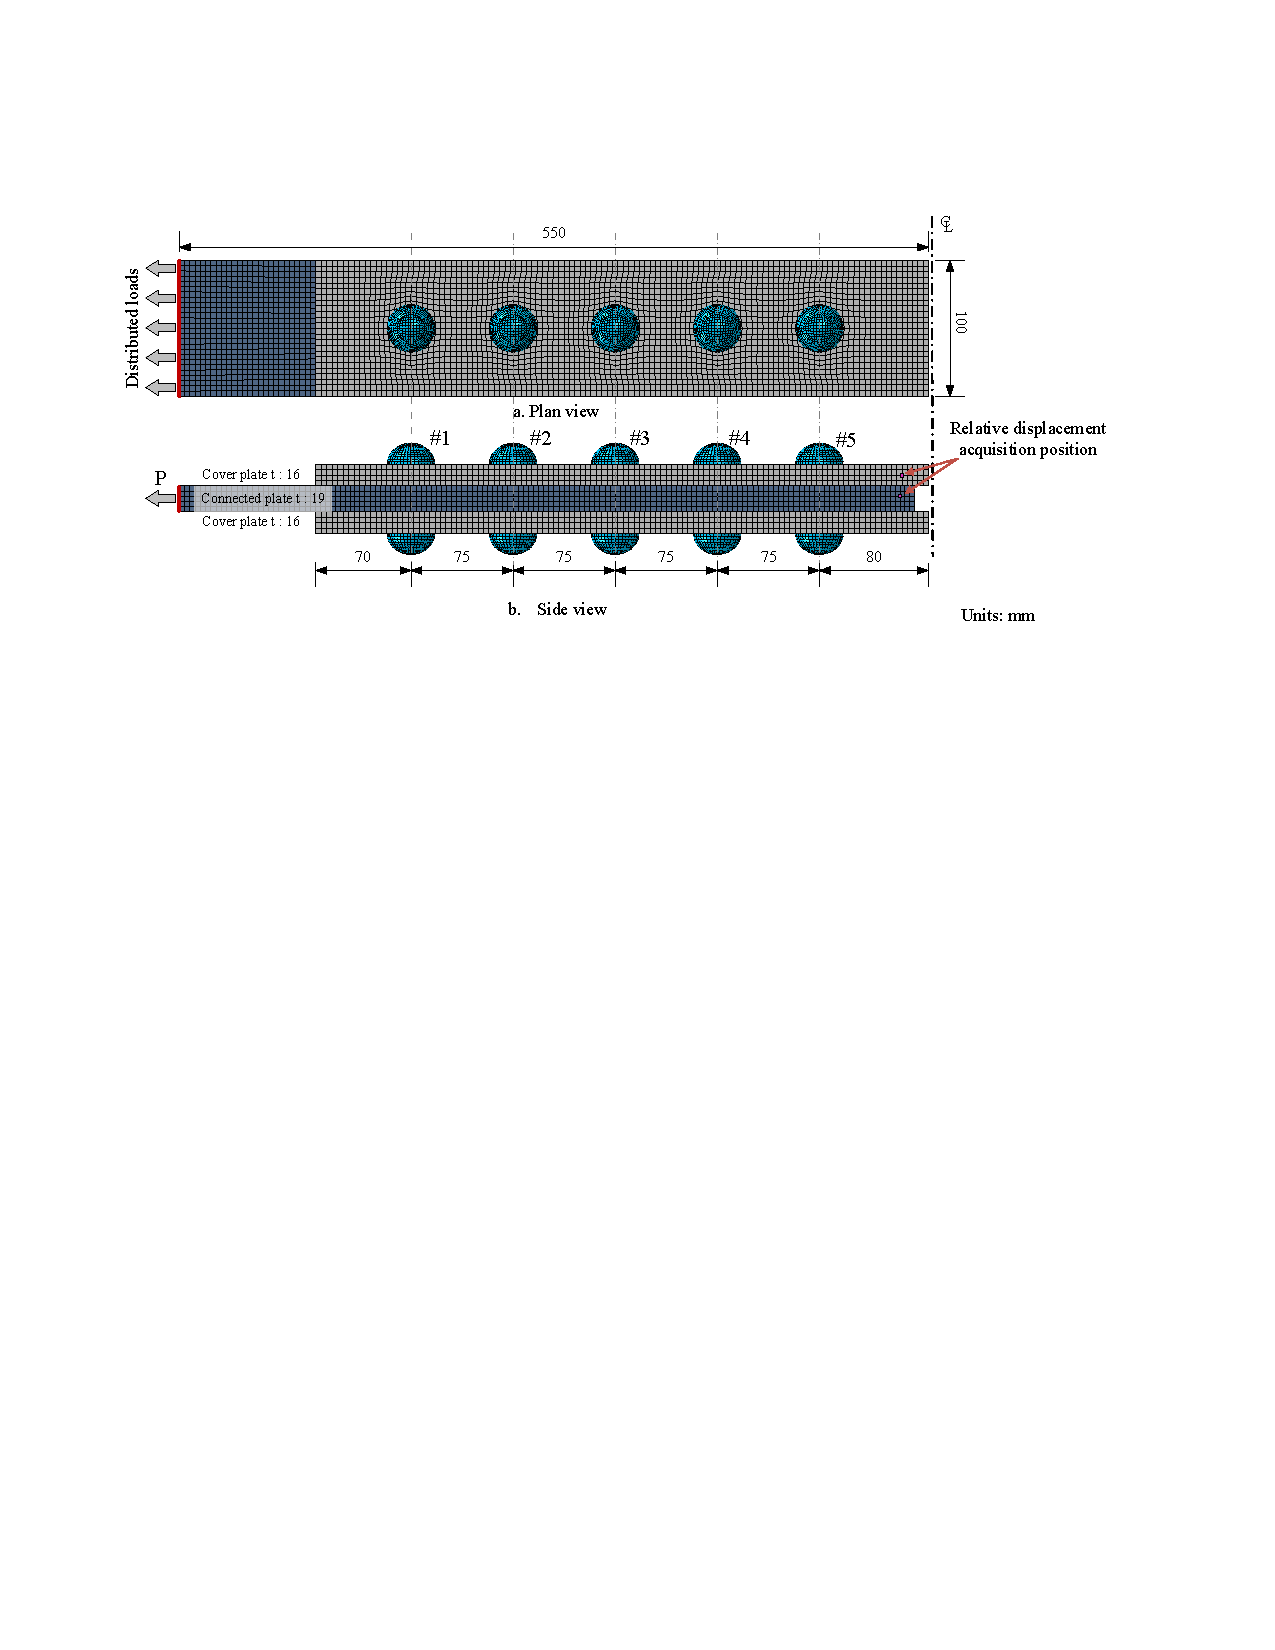
\includegraphics[width=0.9\textwidth]{imgs/ch4/fig-l5.pdf}
    \caption{Schematic illustration of FE model}
    \label{fig-l5}
\end{figure}

The mechanical properties and stress–strain curves of the steel plates, rivets, and bolts are shown in Table \ref{tab-l1} and Fig. \ref{fig-l6}. Material properties were used nominal values of recommendation by Japanese Industrial Standards. In fact, the properties were based on the rivets and steel plates used in the target bridge, as well as those of high-strength bolts utilized in most Japanese bridges.

\begin{table}[htbp]
\centering
\caption{Summary of material properties} \label{tab-l1}
\begin{tabular}{@{}cccccc@{}}
\toprule
Member &
  Material &
  \begin{tabular}[c]{@{}c@{}}Yong's modulus E\\ {[}Mpa{]}\end{tabular} &
  Poisson's ratio $v$ &
  \begin{tabular}[c]{@{}c@{}}$f_y$\\ {[}Mpa{]}\end{tabular} &
  \begin{tabular}[c]{@{}c@{}}$f_u$\\ {[}Mpa{]}\end{tabular} \\ \midrule
Rivet & SV400 & 200,000 & 0.3 & 245 & 500  \\
Bolt  & F10T  & 200,000 & 0.3 & 900 & 1000 \\
Plate & SM570 & 200,000 & 0.3 & 460 & 520  \\ \bottomrule
\end{tabular}
\end{table}

\begin{figure}[htbp]
    \centering
    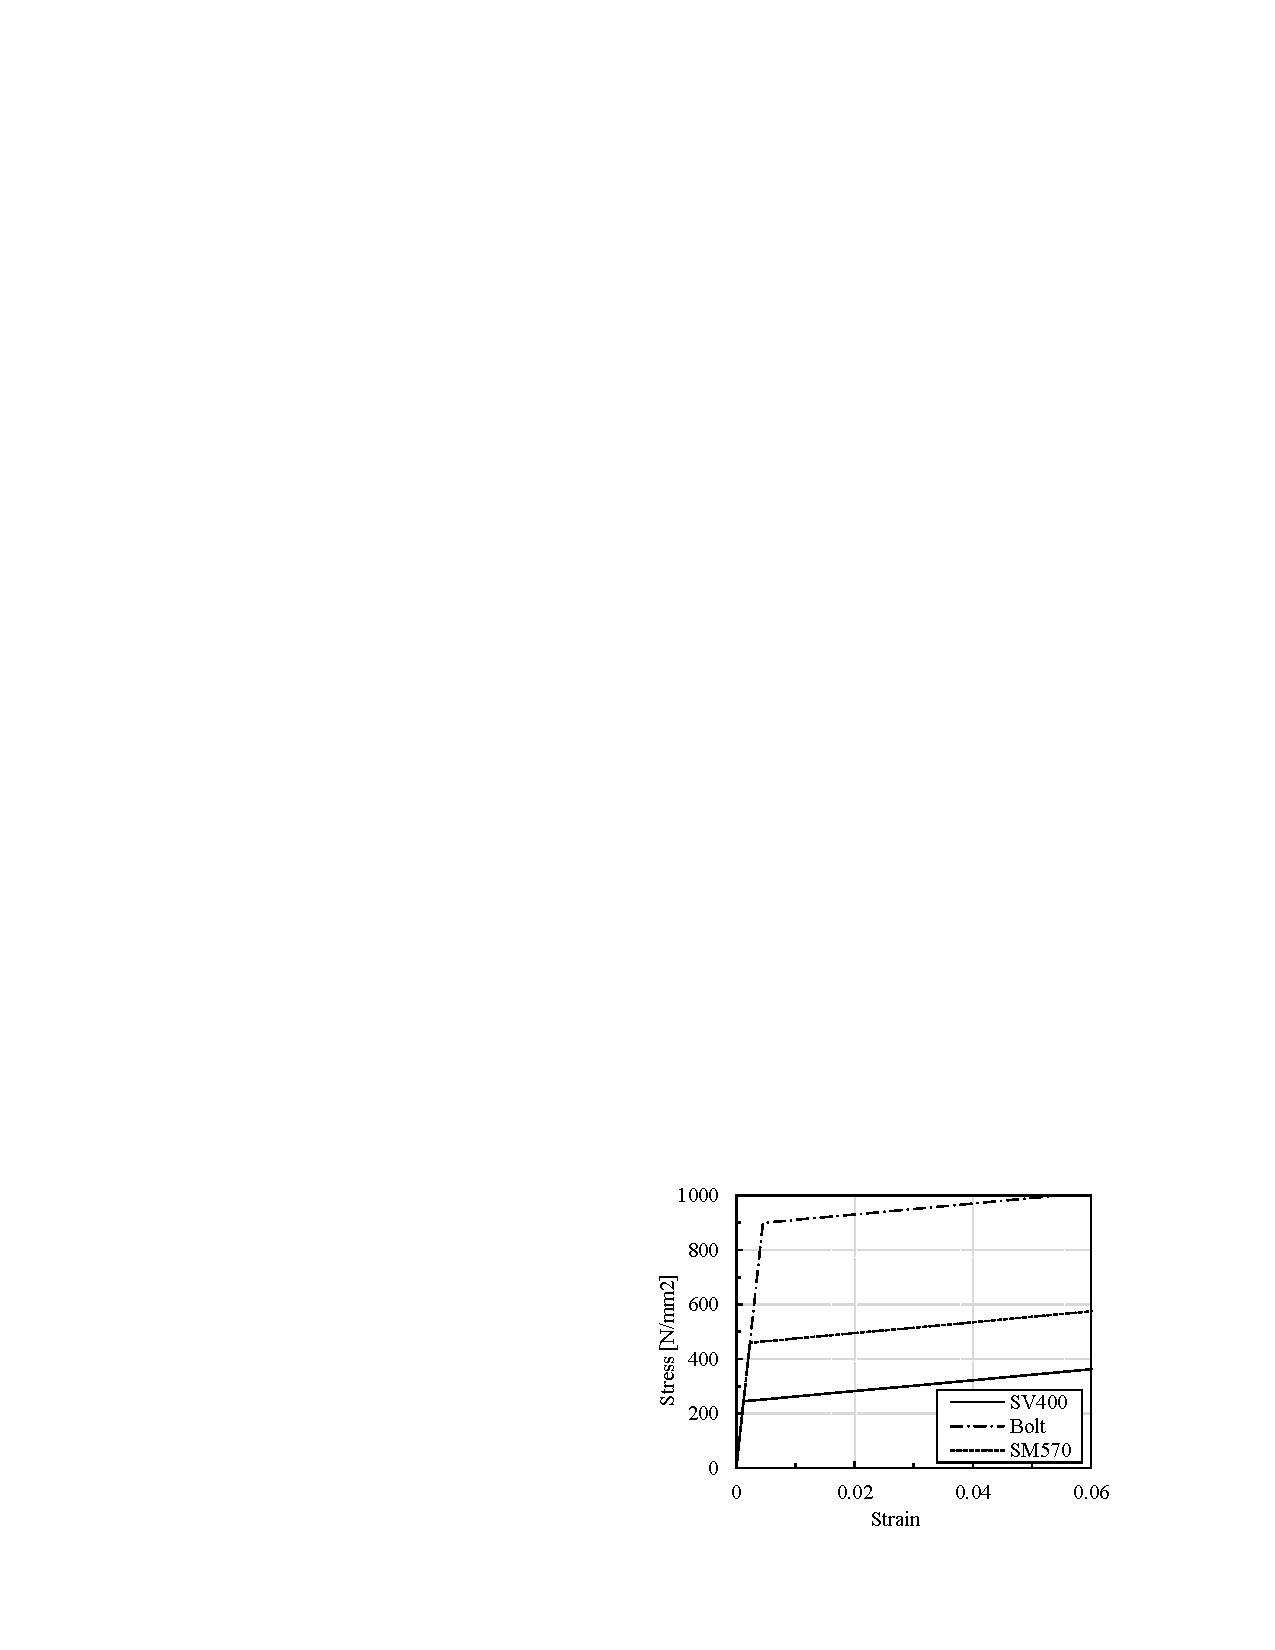
\includegraphics[width=0.6\textwidth]{imgs/ch4/fig-l6.pdf}
    \caption{Stress–strain curves of materials considered in present study}
    \label{fig-l6}
\end{figure}

It is previously demonstrated that a clamping force exists in rivets and that it is positively correlated with the rivet shank length \cite{Leonetti2020RivetBridges}. However, significant scattering occurs in the clamping force generated by each rivet, and bridge designers generally disregard the clamping force of the rivet. The clamping force generated by the rivet was not considered in the present study to simplify the evaluation of the rivet transfer force.

A penalty friction formulation from Abaqus was used in the FE model to simulate the Coulomb friction behavior. In the Chapter \ref{ch3}, the slip test was conducted for 90-year-old riveted joints, and the results showed that the average slip coefficient
of the riveted joints was 0.27. The friction coefficient between the connected and cover plates in this model was set to the same value of 0.27.

\subsection{FE analysis case}

To elucidate the load redistribution mechanism of the joint when individual rivets are replaced, the location of the replaced rivet was analyzed in the present study. Table \ref{tab-l2} shows the analysis cases, where RP1 represents the replacement of rivet \#1.

\begin{table}[htbp]
\centering
\caption{Analysis cases}\label{tab-l2}
\begin{tabular}{@{}cccccc@{}}
\toprule
\multirow{2}{*}{Case} & \multicolumn{5}{c}{Fastener location} \\ \cmidrule(l){2-6} 
                      & \#1   & \#2   & \#3   & \#4   & \#5   \\ \midrule
RP0                   & ◯     & ◯     & ◯     & ◯     & ◯     \\
RP1                   & ▲     & ◯     & ◯     & ◯     & ◯     \\
RP2                   & ◯     & ▲     & ◯     & ◯     & ◯     \\
RP3                   & ◯     & ◯     & ▲     & ◯     & ◯     \\
RP5                   & ◯     & ◯     & ◯     & ◯     & ▲     \\ \midrule
\multicolumn{6}{r}{◯: Rivet; ▲: HSB}                         
\end{tabular}
\end{table}

\begin{table}[htbp]
\centering
\caption{Design resistance (units: kN)}\label{tab-l3}
\begin{tabular}{@{}ccccc@{}}
\toprule
    & $F_{y}$ & $F_{u}$ & $F_{b}$ & $F_{v}$ \\ \midrule
RP0 & 668.6       & 755.8     & 2786.2   & 1214.5   \\ \bottomrule
\end{tabular}
\end{table}

Table \ref{tab-l3} lists the riveted joint’s (RP0) design resistance. Both the riveted joint and the hybrid joint was failure by cross-sectional fracture. The net cross-section yield resistance $F_{y}$, ultimate net cross section resistance $F_{u}$, ultimate bearing resistance $F_{b}$, and ultimate rivet shear resistance $F_v$ are calculated using flowing equation.

\begin{equation*}
    F_y = (w-d_0)tf_y
\end{equation*}
\begin{equation*}
    F_u = (w-d_0)tf_u
\end{equation*}
\begin{equation*}
    F_b = 2.4ndtf_u
\end{equation*}
\begin{equation*}
    F_u = nmA_sf_{ur}
\end{equation*}

\subsection{Reproduction of construction step}
A step analysis was conducted in this study to evaluate the load redistribution within the riveted joint after removing the individual rivets. The steps involved in the analysis are summarized in Table \ref{tab-l4}.

\begin{table}[htbp]
    \centering
    \caption{Steps involved in analysis}\label{tab-l4}
    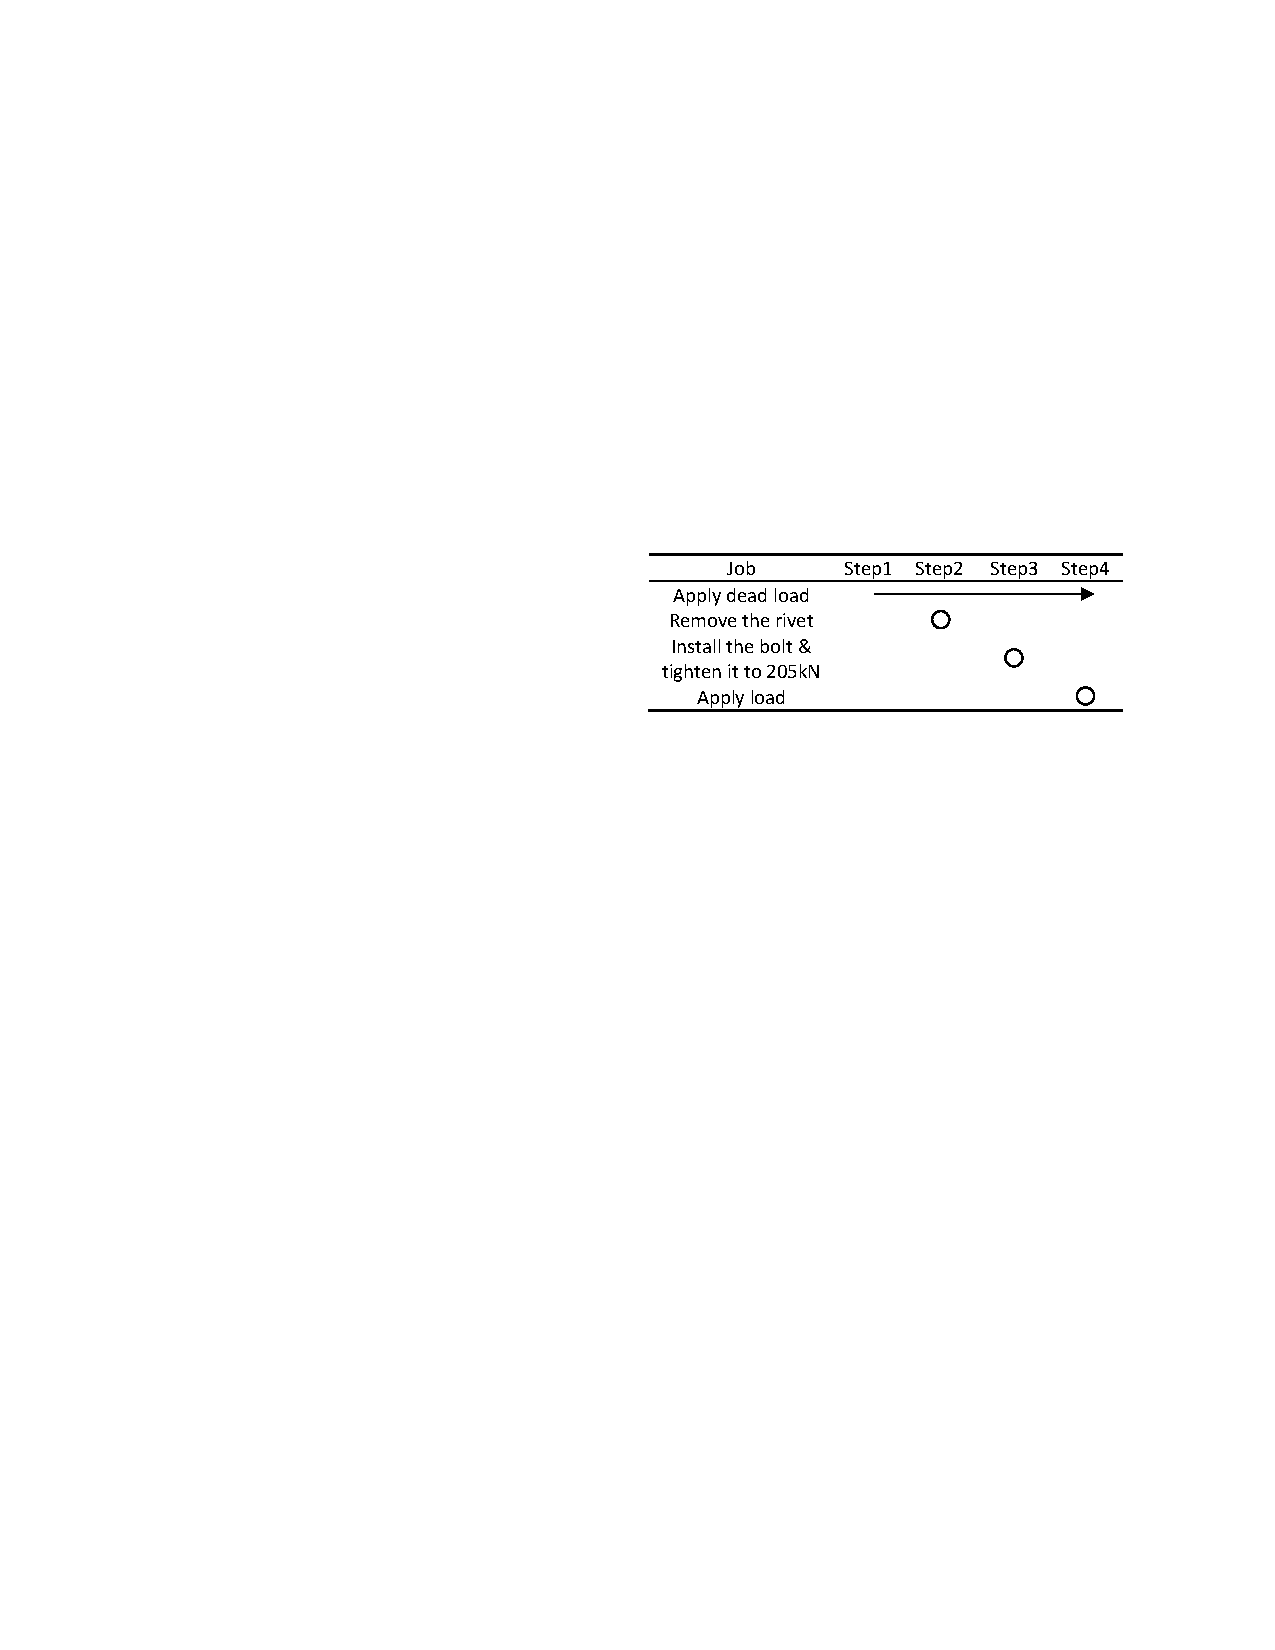
\includegraphics[width=0.7\textwidth]{imgs/ch4/tab-l4.pdf}
\end{table}

The dead load was 72.5 kN, as calculated from the design dead load stress of the rivet girder’s cross section. In step 2, the model change interaction was conducted in Abaqus to reproduce the rivet removal. In step 3, the bolt was installed and tightened to 205 kN. In step 4, the forced displacement was used to apply the live load. The stress contour maps for each step are shown in Fig. \ref{fig-l7}.


\begin{figure}[htbp]
    \centering
    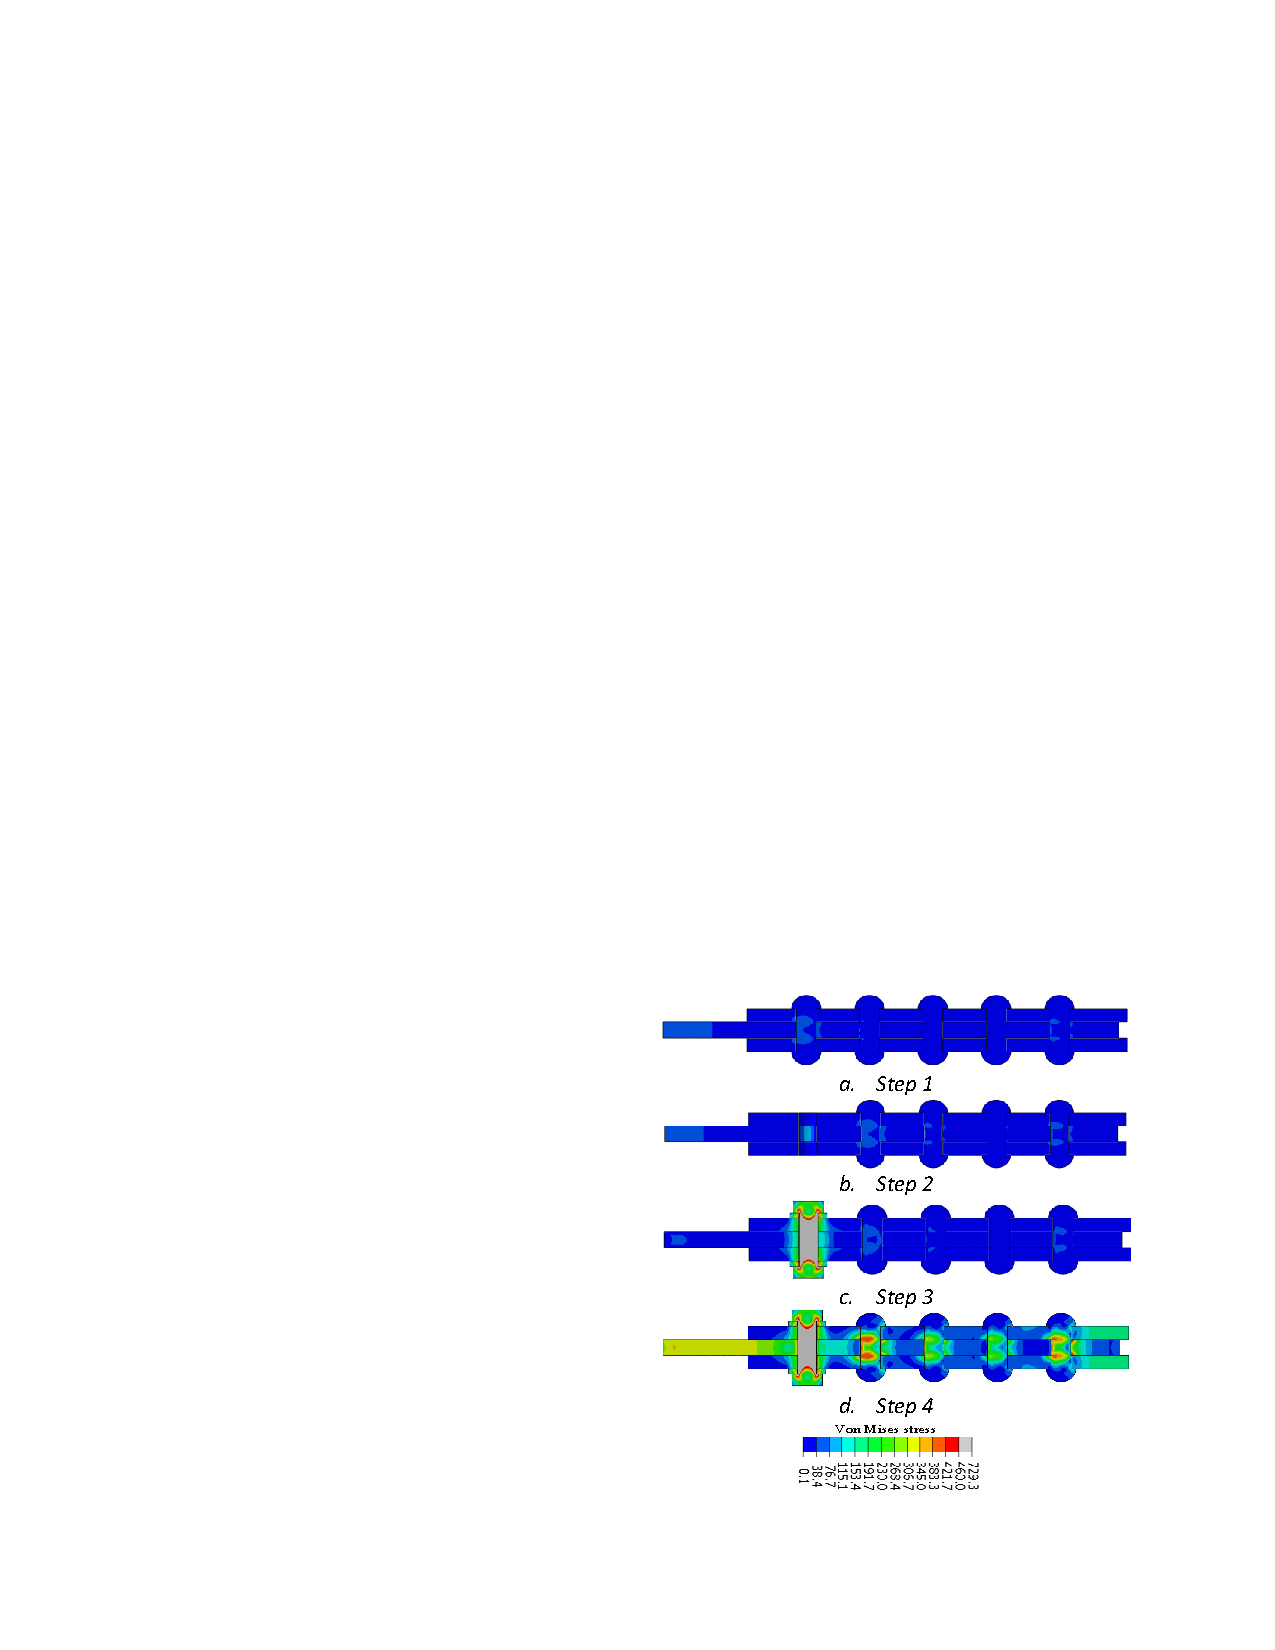
\includegraphics[width=0.7\textwidth]{imgs/ch4/fig-l7.pdf}
    \caption{Steps for reproducing construction (RP1 case)}
    \label{fig-l7}
\end{figure}

\subsection{Results and discussions}

\subsubsection{Load sharing of each rivet (step 2)}

Fig. \ref{fig-l8} shows the load distribution of each fastener before and after rivet removal. The vertical axis represents the bearing resistance of each rivet, and the horizontal axis represents the rivet position. The green / orange bars represent the bearing resistance of the rivet before and after a
certain rivet is removed.

\begin{figure}[htbp]
    \centering
    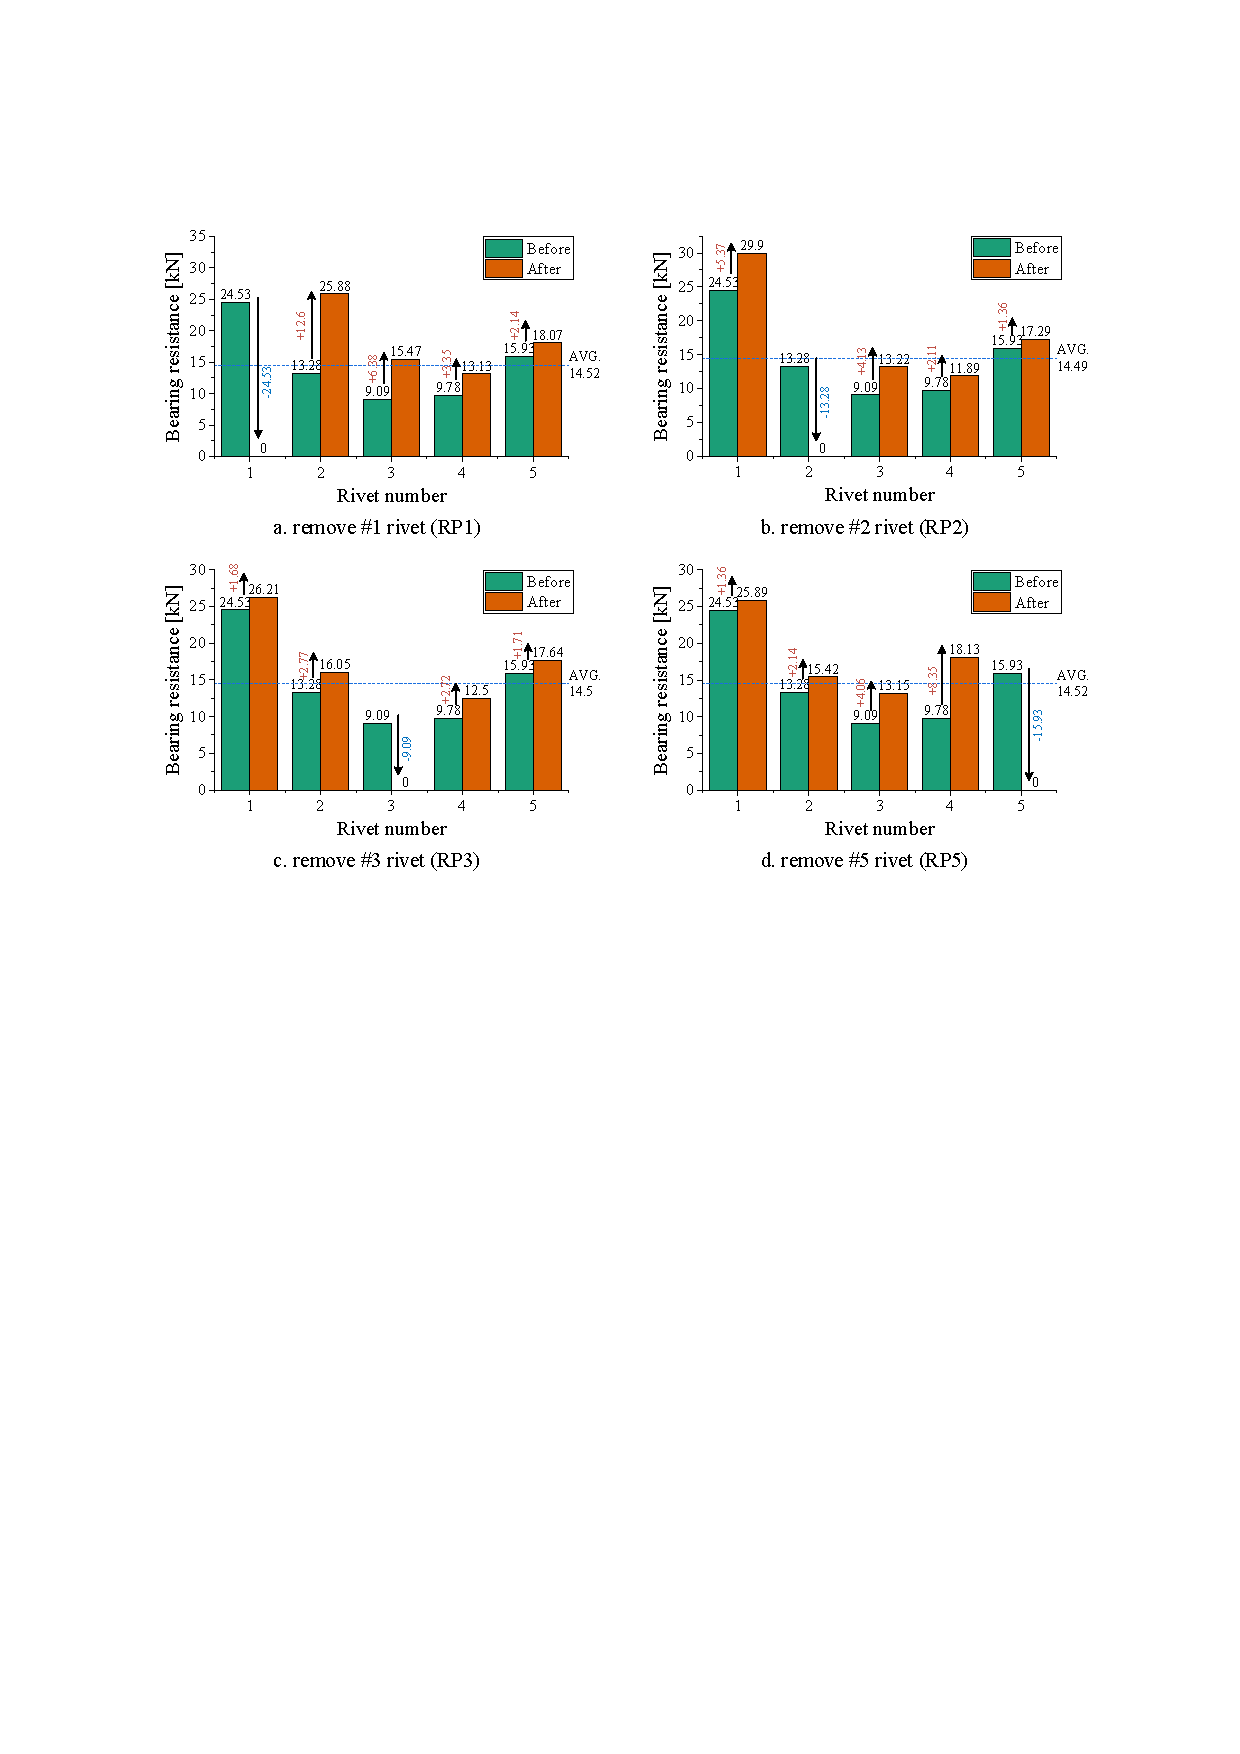
\includegraphics[width=\textwidth]{imgs/ch4/fig-l8.pdf}
    \caption{Load sharing of each fastener within dead load (before and after removing rivet)}
    \label{fig-l8}
\end{figure}

Table \ref{tab-l5} shows the load redistribution among the remaining rivets after the removal of an individual rivet.

\begin{table}[htbp]
    \centering
    \caption{Load redistribution of removed riveted [\%]}\label{tab-l5}
    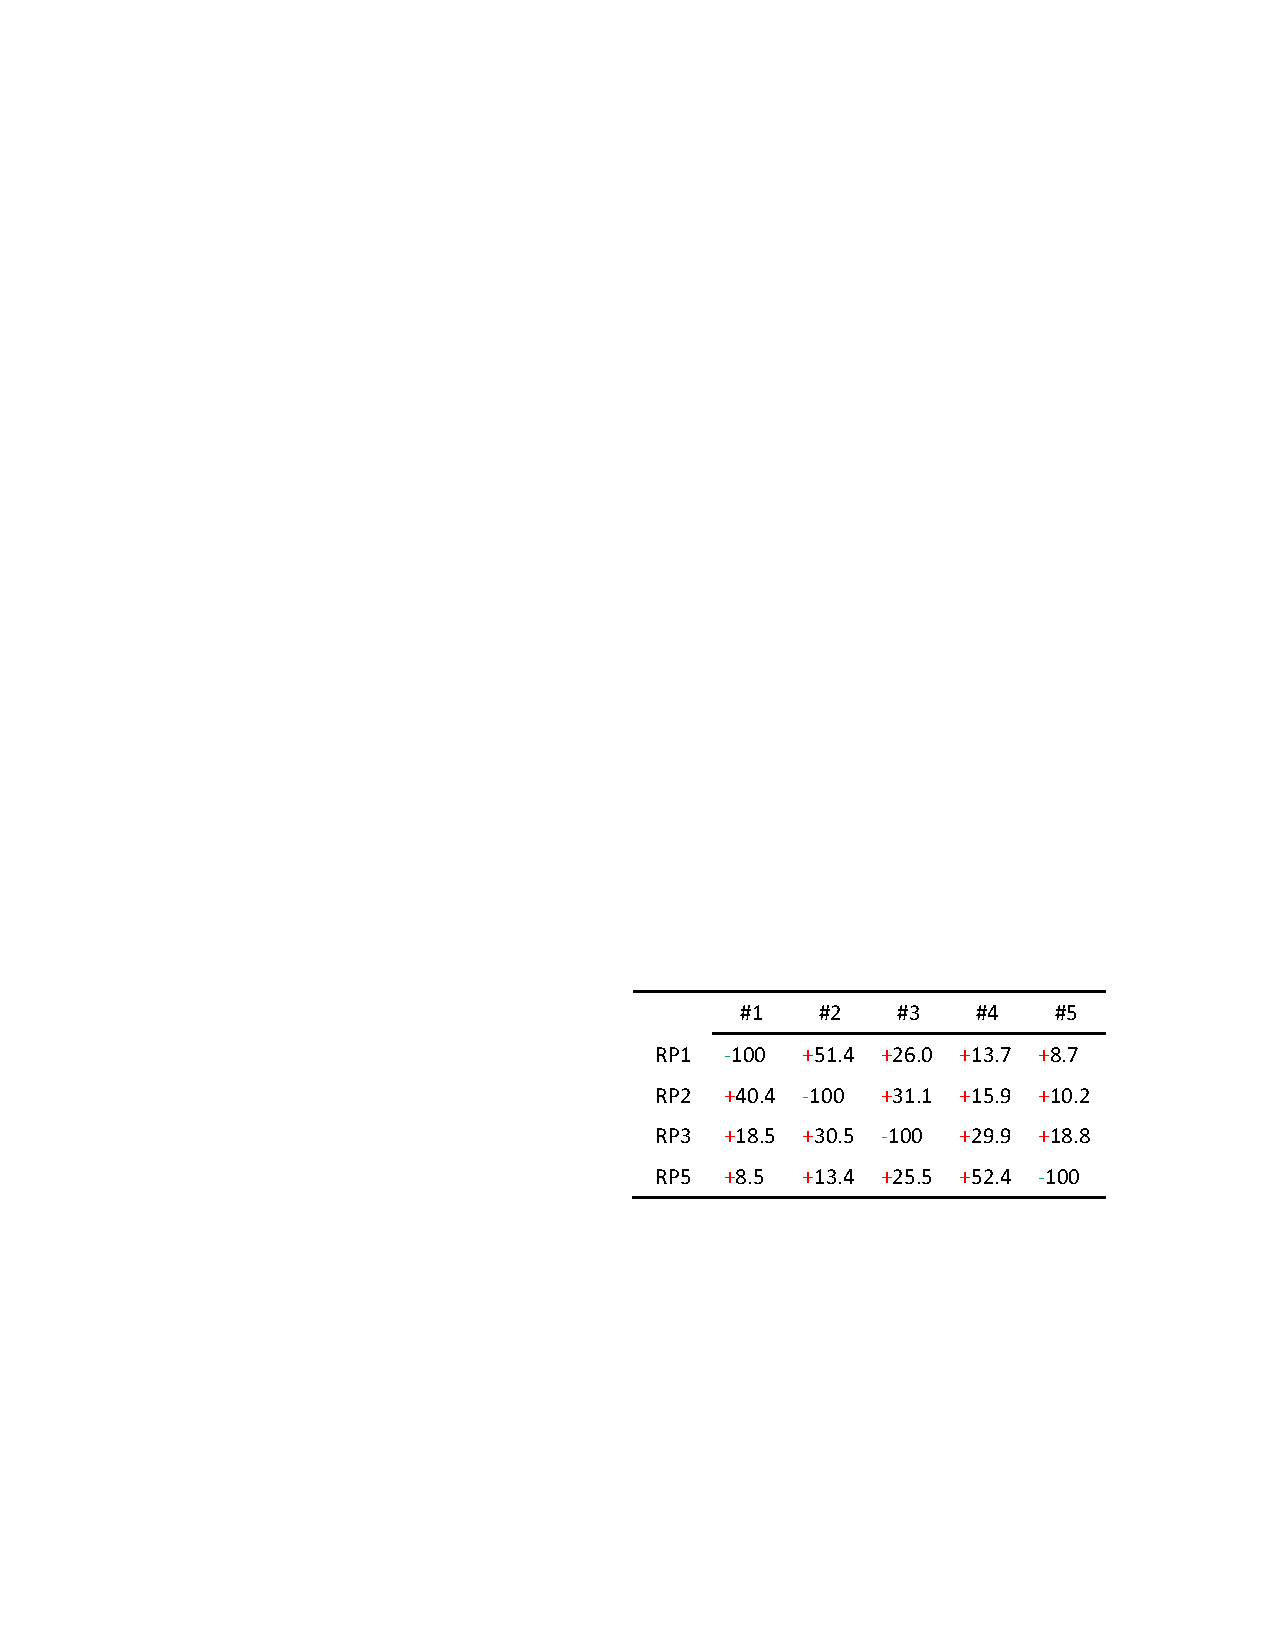
\includegraphics[width=0.6\textwidth]{imgs/ch4/tab-l5.pdf}
\end{table}

The bearing resistance of each rivet was calculated using the contact pressure on the rivet hole surface. The friction resistance of the bolt was calculated using the frictional stress on the top surface. The hole and top surfaces are shown in Fig. \ref{fig-l9}.

\begin{figure}[htbp]
    \centering
    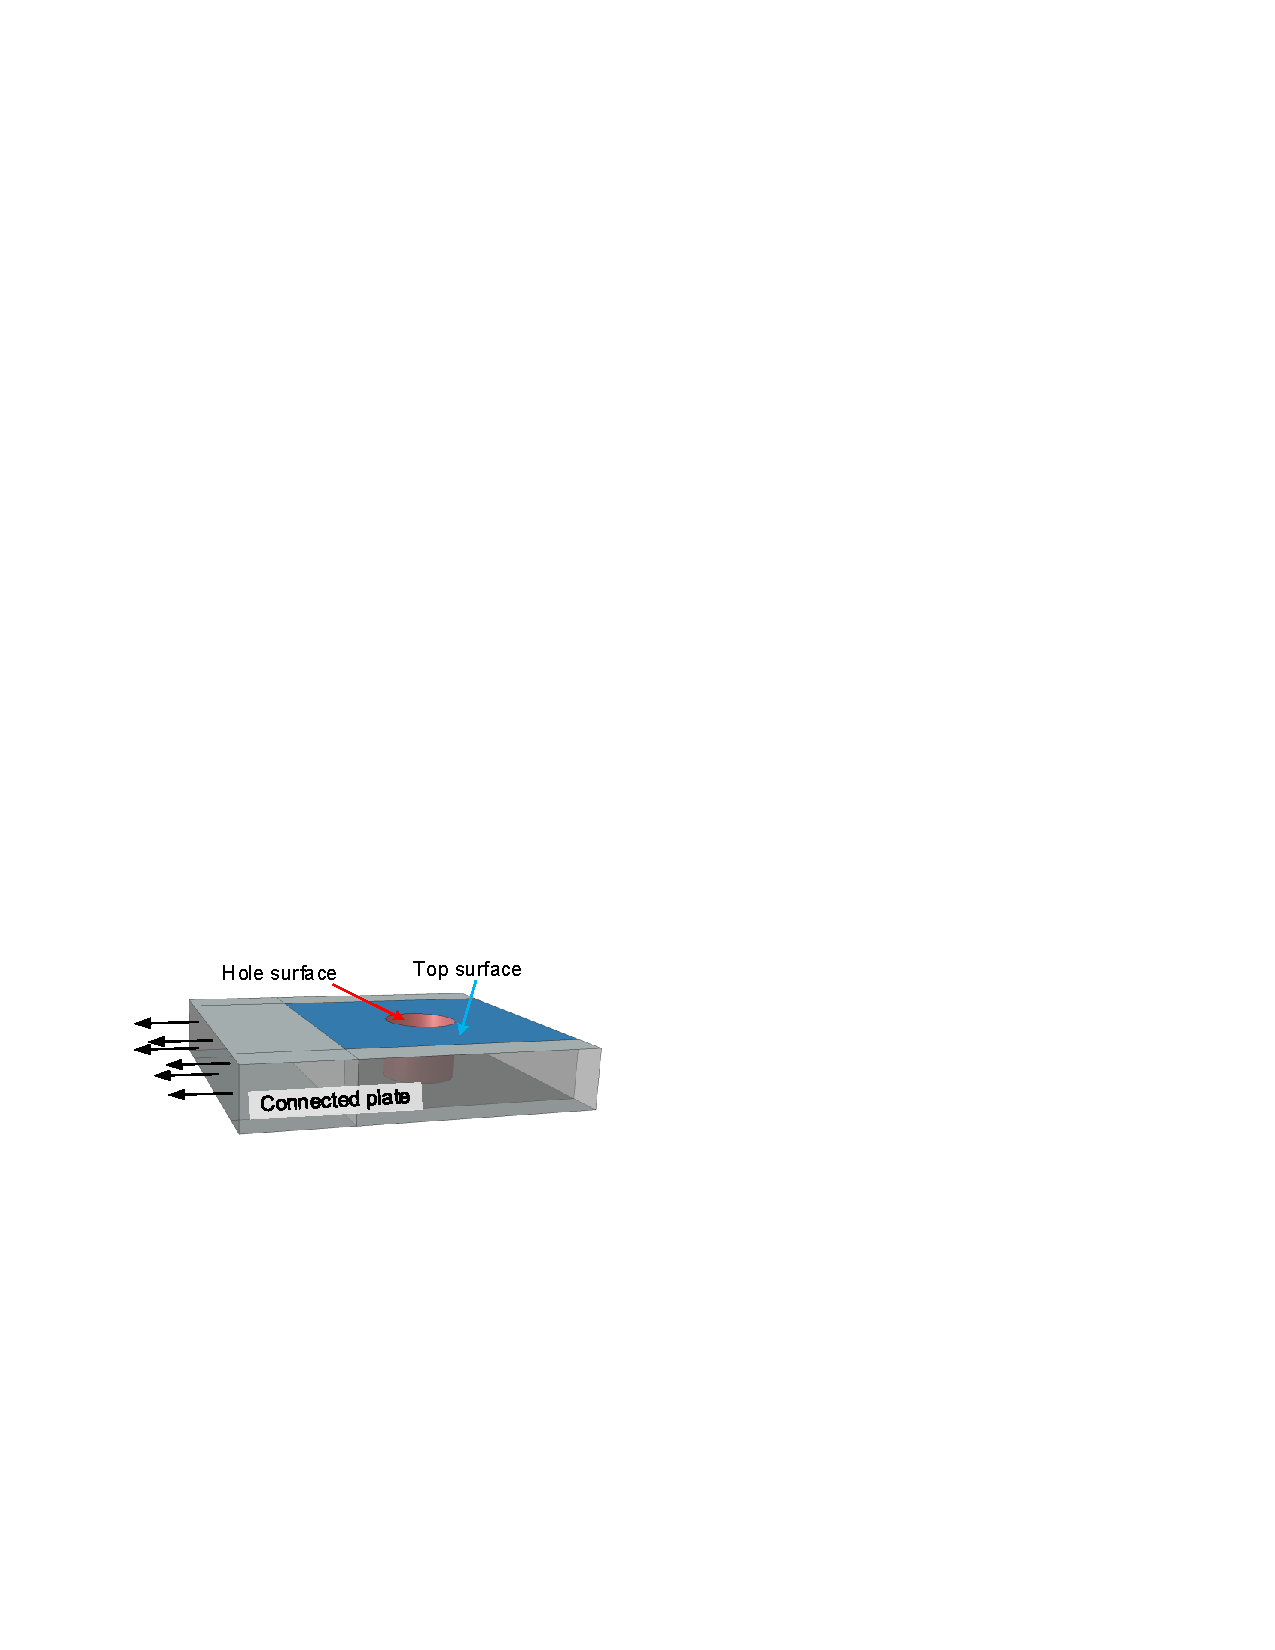
\includegraphics[width=0.7\textwidth]{imgs/ch4/fig-l9.pdf}
    \caption{Location where bearing/friction resistance is calculated}
    \label{fig-l9}
\end{figure}

As shown in Fig. \ref{fig-l8}.a, the bearing resistance (24.53 kN) originally transferred by rivet \#1 was redistributed among the remaining four rivets. Approximately 51\% (12.6 kN / 24.53 kN) of the bearing resistance of rivet \#1 was transferred to rivet \#2, which was the closest rivet to \#1. The bearing resistance of rivet \#2 increased from 13.28 to 25.88 kN. The bearing resistances of rivets \#3, \#4, and \#5 were redistributed by 26\% (6.38 kN / 24.53 kN), 13.7\%, and 8.7\% of the \#1 rivet bearing resistance, respectively.

In addition, it was discovered that the removal of rivet \#1 was based a similar load redistribution mechanism to that of the removal of rivet \#5, as shown in Table \ref{tab-l5}.

As shown in Fig. \ref{fig-l8}.c, removing middle rivet \#3 caused its bearing resistance to be distributed evenly among the remaining rivets.

\subsubsection{Resistance of each fastener}

Fig. \ref{fig-l10} shows the relationship between each fastener’s reaction force and displacement for each case from steps 2 to 4. $P_{s1}$ is the maximum reaction force of the bolt. In step 2, the residual deformation due to the dead load was disregarded, and loading was commenced from 0 kN.

\begin{figure}[htbp]
    \centering
    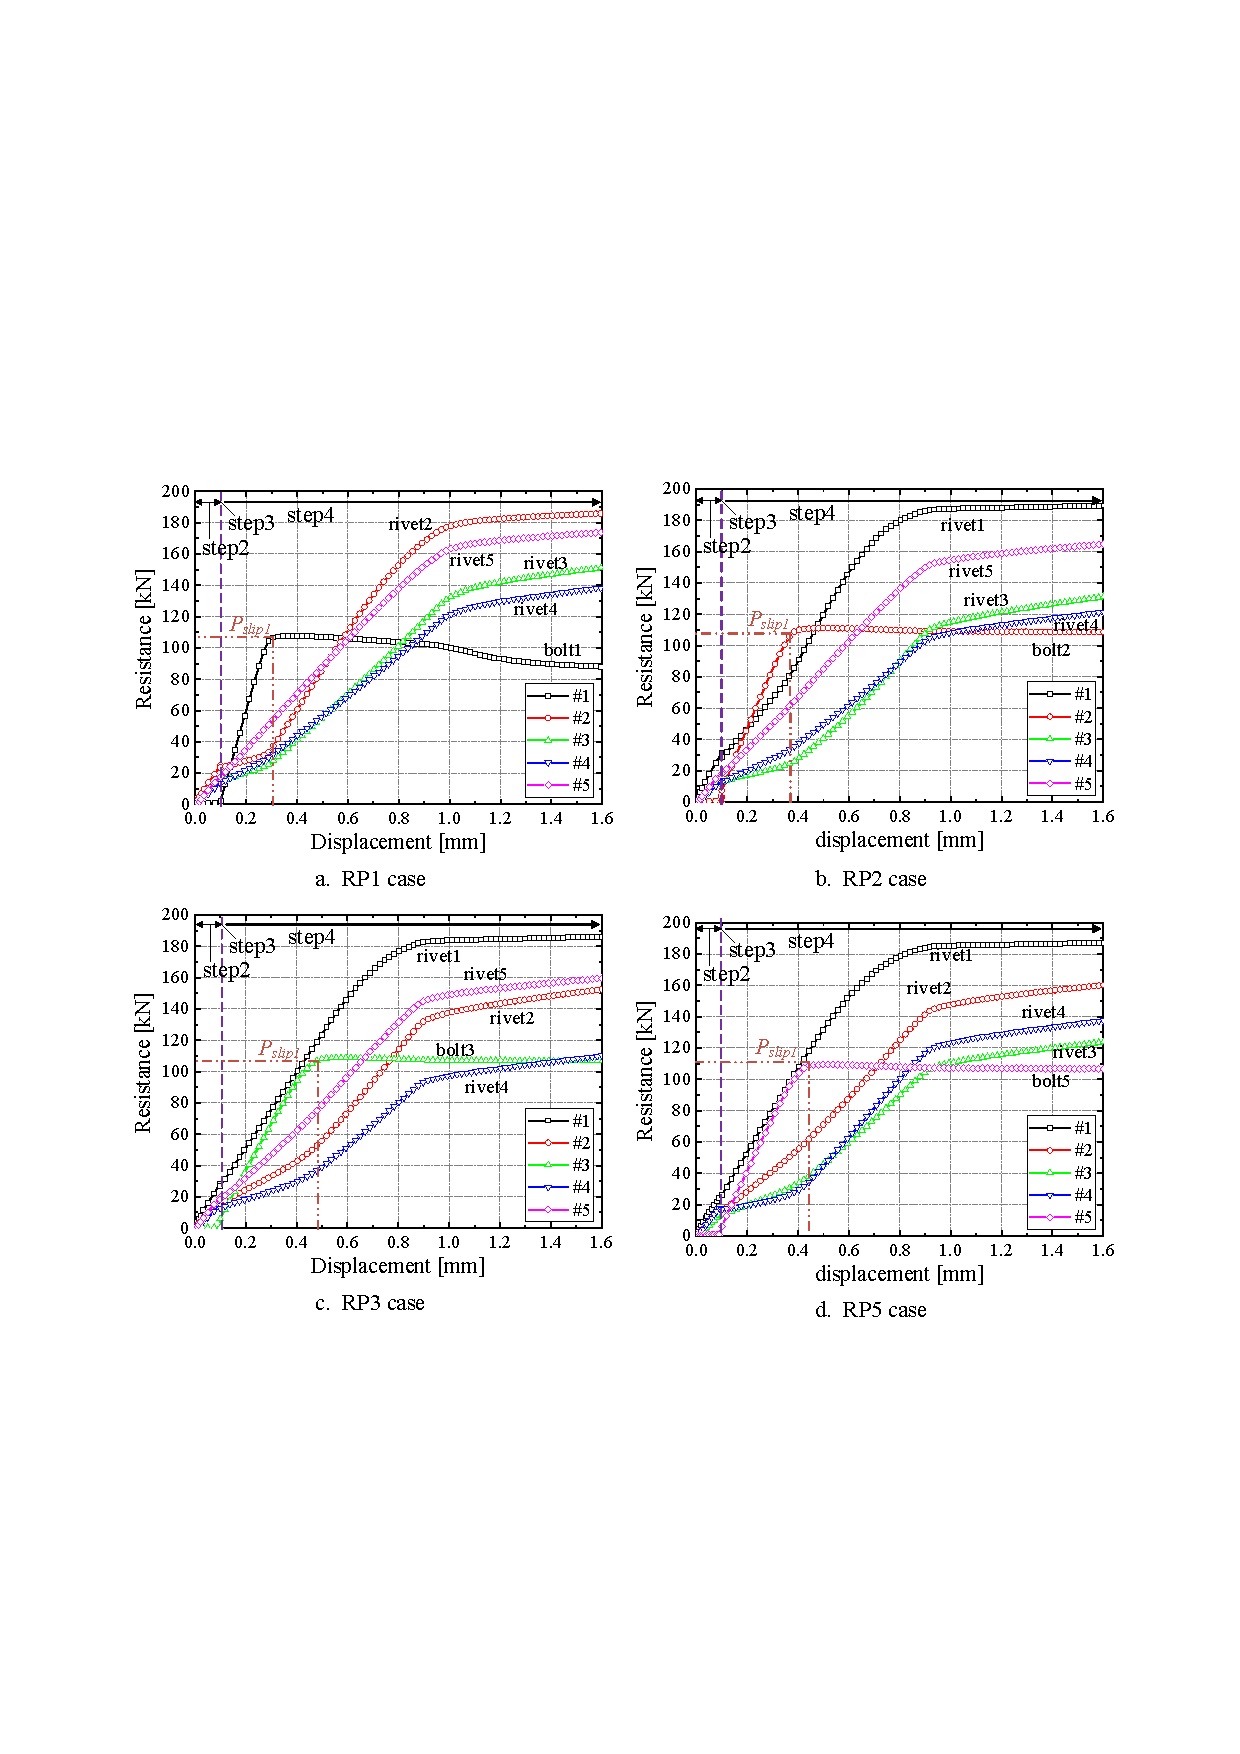
\includegraphics[width=\textwidth]{imgs/ch4/fig-l10.pdf}
    \caption{Relationship between each fastener’s reaction force and displacement}
    \label{fig-l10}
\end{figure}

As shown in Fig. \ref{fig-l10}, before the bolt’s resistance reached $P_{s1}$, rivets near the replaced rivet were affected more by the newly fastened bolt, thereby rendering the rivet’s load transfer less efficient. efficient. Meanwhile, the rivets distant from the bolt were almost unaffected. For example, as shown in Fig. \ref{fig-l10}.a, where rivet \#1 was replaced by a bolt, the curve of rivet \#5 barely changed, and the slope of rivet \#2 decreased after the rivet was replaced.

When the reaction force of the bolt exceeded $P_{s1}$, the bolt no longer transferred forces. Meanwhile, the curves of the rivets that were adjacent to the bolt changed, resulting in a more efficient load transfer. However, the more distant rivets were unaffected.

\subsubsection{Overall mechanical behavior}

Fig. \ref{fig-l11} shows the relationship between load and displacement for each case. As shown in the figure, the overall mechanical behavior was similar to that of RP0 and RP1. This might be because in RP1, bolt \#1 transferred more load to the cover plate via friction, thereby relieving the net cross-section stress in the connected plate.

\begin{figure}[htbp]
    \centering
    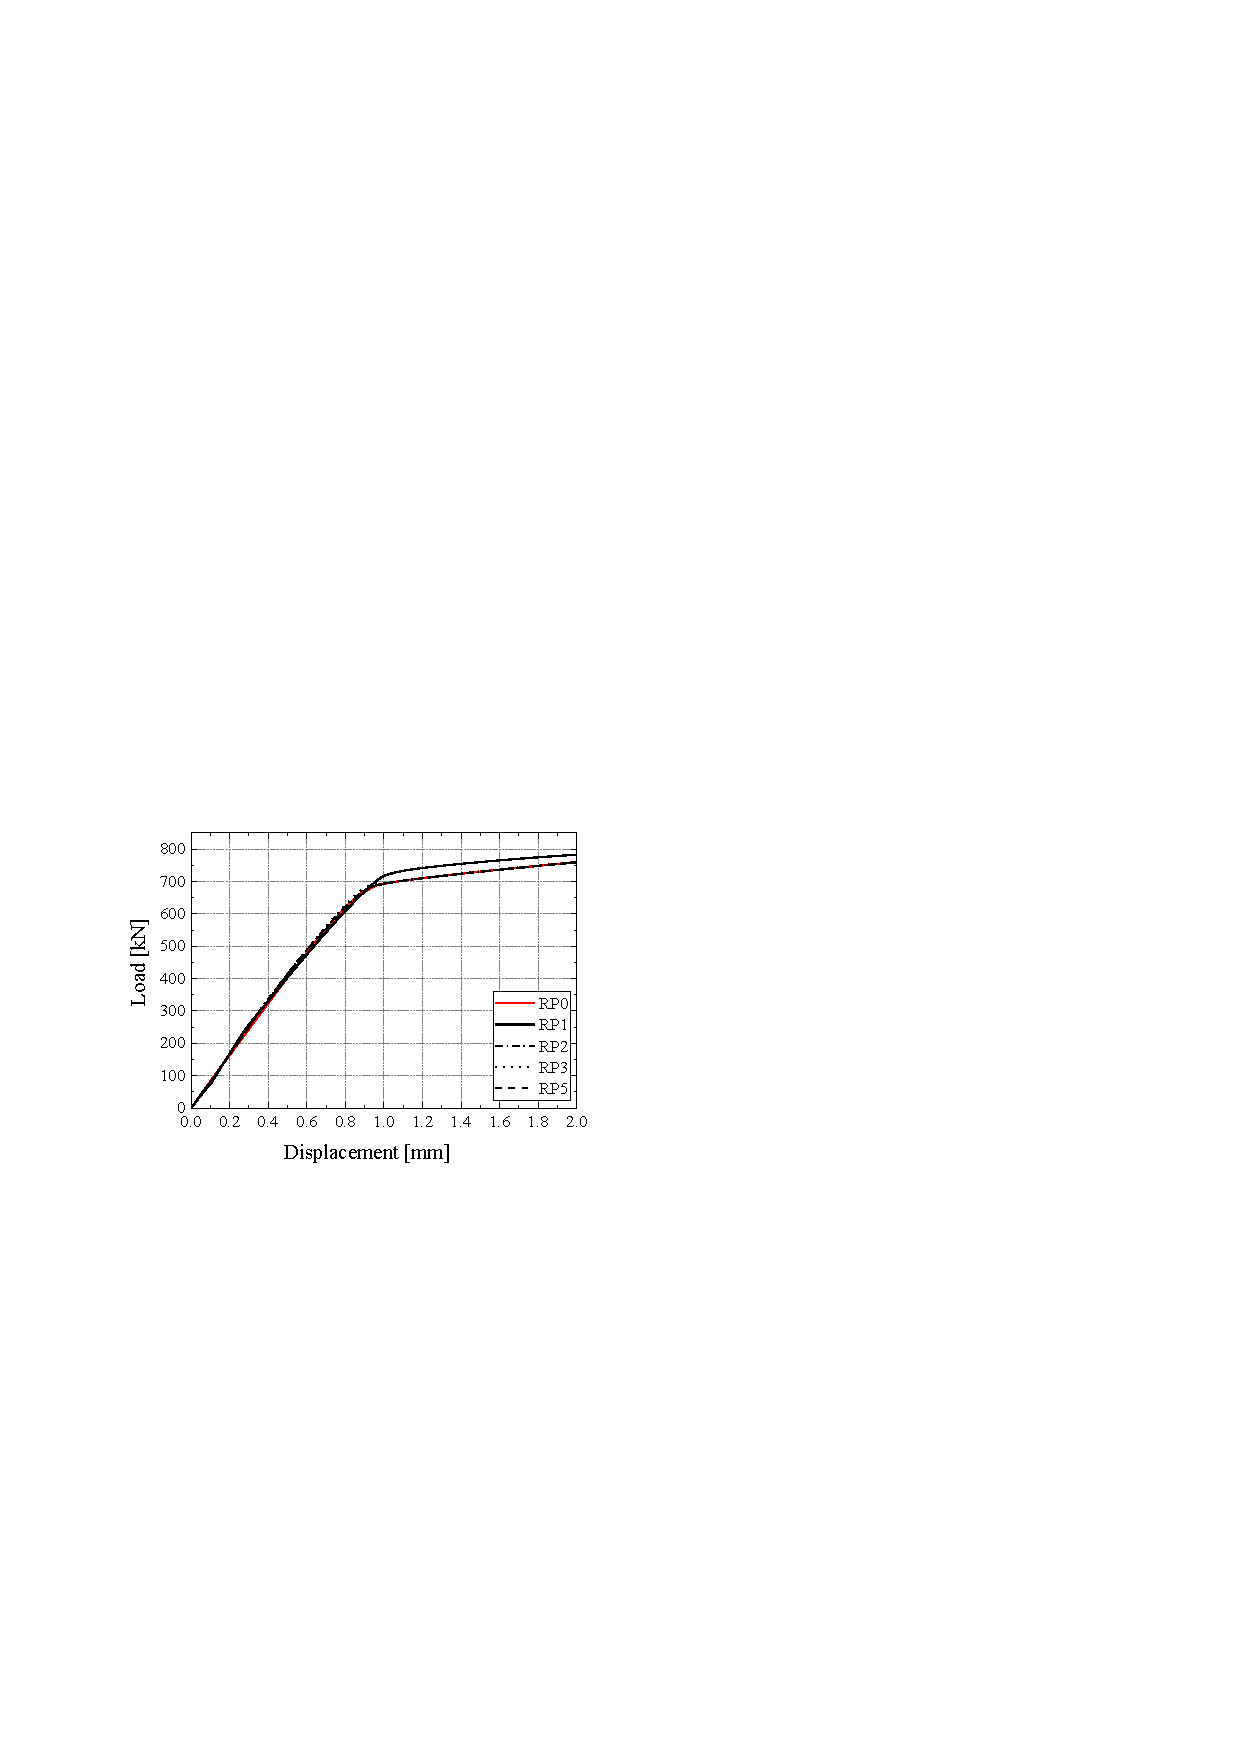
\includegraphics[width=0.6\textwidth]{imgs/ch4/fig-l11.pdf}
    \caption{Relationship between each fastener’s reaction force and displacement}
    \label{fig-l11}
\end{figure}

\section{Investigate for The Long Riveted Joint}

In the previous section, in the case of a hybrid joint using three rows of rivets and a high-strength bolt friction connection, although nonlinear behavior is not exhibited until the inner rivet holes plasticize, the degree of plasticization is not uniform and the plasticization zone increases as one moves away from the center of the joint. However, when the number of rivet rows is small, as in the case of the subject studied in section \ref{ch4sec2}, the plasticization bias at each rivet position is small, and it is considered possible to evaluate the plasticization of the rivet holes at the initial stage of nonlinear behavior by multiplying the nominal bearing stress by the number of rivets. However, which discusses only one-row, three-row joints, the number of rivets in a row actually increases, the force acting on the rivets is not uniform, and there is a large possibility that localized yielding will occur first.

\subsection{FE analysis}

Fig. \ref{fig-femodl-5r} shows the FE analysis model and the dimension of the joint. The analysis case are shown in Table \ref{tab-5rcase}, the rivets were replaced with high-strength bolts and the position and number of rivets were used as parameters in the analysis.

The analytical model consists of a total of five rivets. The modeling range of the analytical model is 1/4 model in the direction of the plate width for symmetry. The analytical model consists of an 8-node 3D solid element (reduced integral element) for the joint, splice plate, bolt, and washer. Faying surfaces were set on the joint surfaces between the jointed material and splice plate, bolt and bolt hole, and rivet and rivet hole, and boundary nonlinearities were considered. The rivet hole was modeled as 23.5 mm so that the rivet and the hole wall were in contact beforehand. When replacing the rivet with a high-strength bolt, the bolt hole was left at 23.5 mm.

\begin{figure}
    \centering
    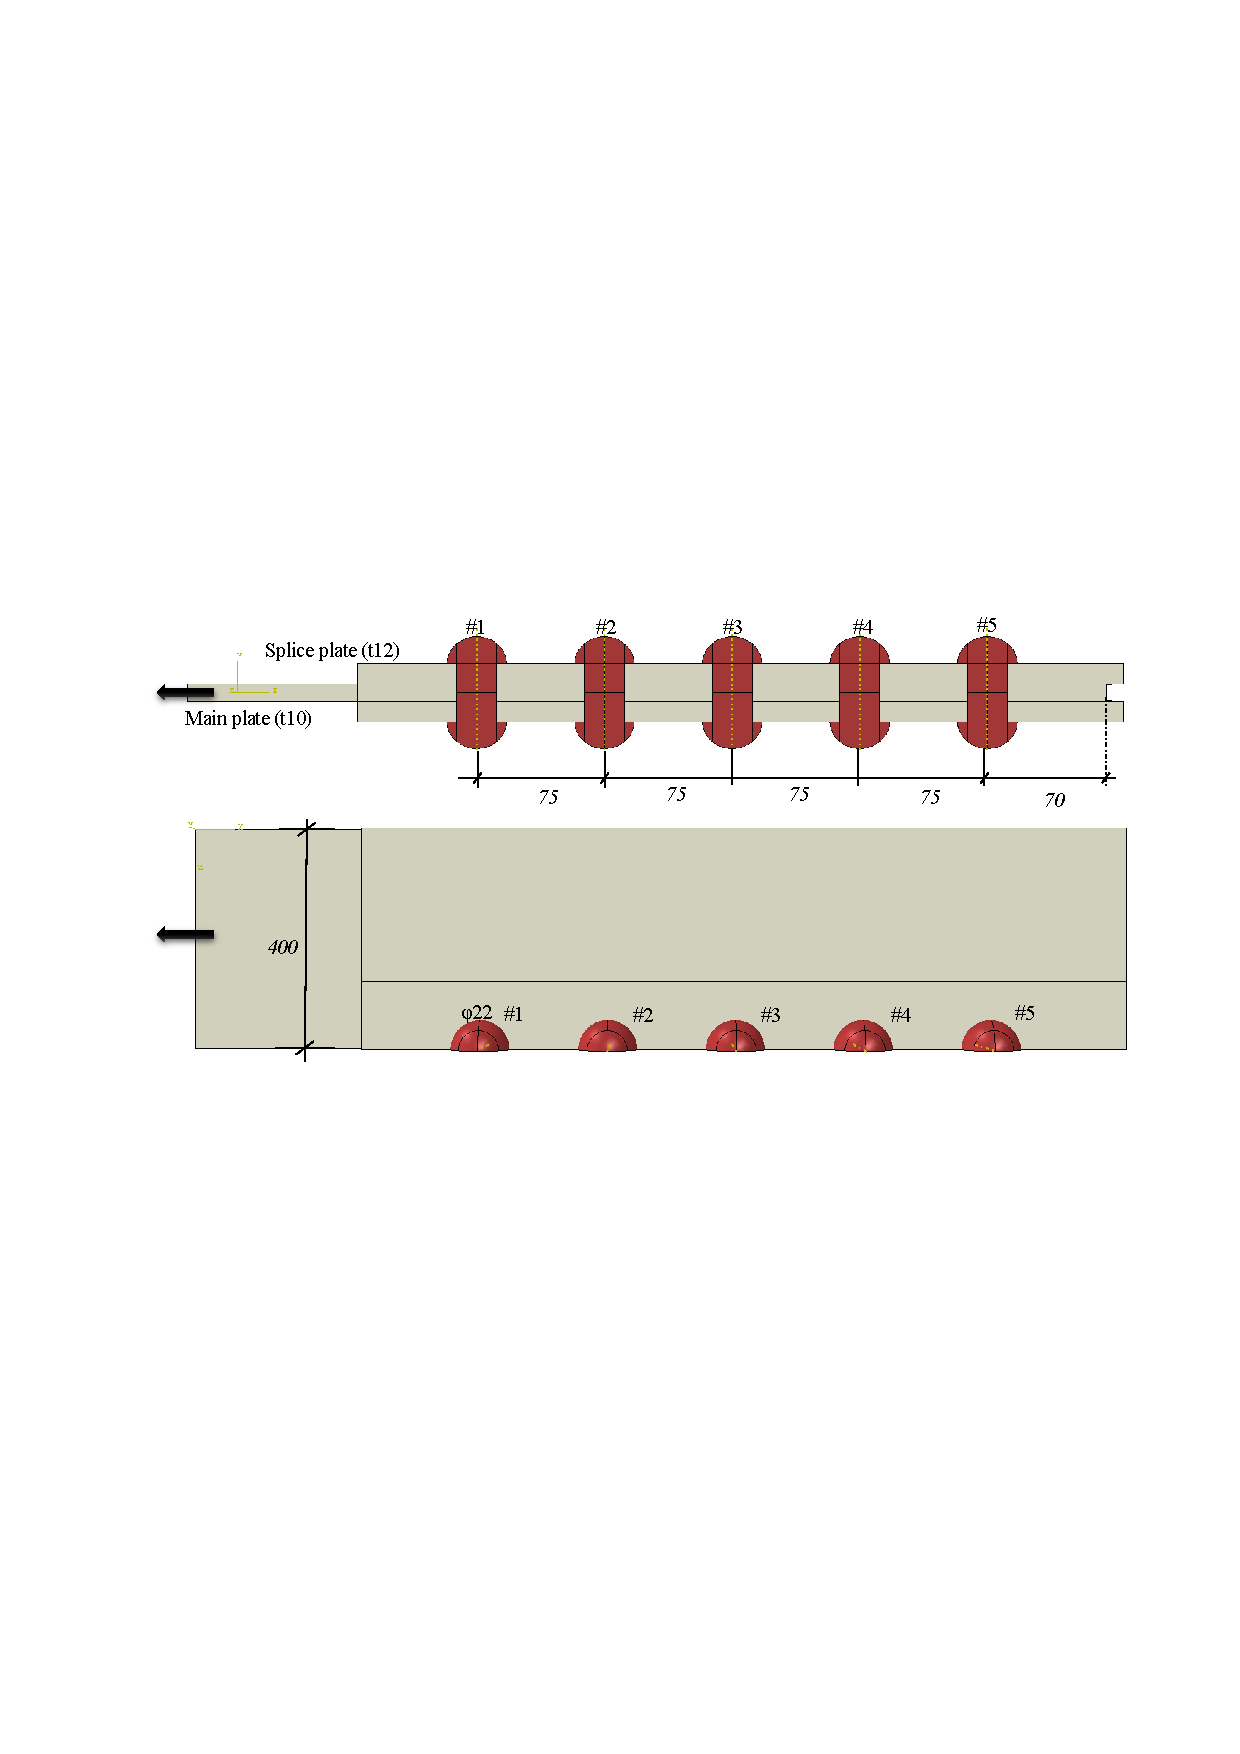
\includegraphics[width=0.9\linewidth]{imgs//ch4/fig-femodl-5r.pdf}
    \caption{FE analysis model}
    \label{fig-femodl-5r}
\end{figure}

\begin{table}[htbp]
\centering
\caption{Analysis cases}\label{tab-5rcase}
\begin{tabular}{@{}cccccc@{}}
\toprule
\multirow{2}{*}{Case} & \multicolumn{5}{c}{Fastener location} \\ \cmidrule(l){2-6} 
                      & \#1   & \#2   & \#3   & \#4   & \#5   \\ \midrule
R5B0                   & ◯     & ◯     & ◯     & ◯     & ◯     \\
R4B1                   & ▲     & ◯     & ◯     & ◯     & ◯     \\
R3B2                   & ▲     &◯     & ◯     & ◯     & ▲     \\
R2B5                   & ▲     & ◯     & ▲     & ◯     & ▲     \\
R0B5                   & ▲     & ▲     & ▲     & ▲     & ▲     \\ \midrule
\multicolumn{6}{r}{◯: Rivet; ▲: HSB}
\end{tabular}
\end{table}

In the analysis, an initial axial force was introduced to the rivet and high-strength bolt in Step 1, and a tensile force due to forced displacement was applied to the end of the material to be welded in Step 2. Although some axial force was actually introduced due to cooling and shrinkage of the rivet, this force was not taken into account in the analysis. However, this axial force was not taken into account in this analysis.

The conditions of material properties and coefficient of friction used for the analysis are the same as in the previous section.

\subsection{Result and discussion}

\subsubsection{Displacement}

Fig.\ref{fig-5rld} shows the The relationship between load and displacement of all the 5-row case. The location of the load and displacement acquisition is where the forced displacement is given.

The initial stiffness of the joint depends on the number of high-strength bolts. The higher the number of high-strength bolts, the higher the initial stiffness of the joint. This is consistent with the results in section \ref{ch4sec2}. In the R0B5 case, slip was observed, but in the case with rivets, no slip was observed because the joint was transmitting the load by bearing. In the case with rivets and joints with rivets, the joint begins to exhibit nonlinear behavior when the displacement is about 1.8 mm. This nonlinear behavior is considered to be caused by the deformation of the hole due to yielding around the hole in the main plate. The more fasteners resist the load by bearing, the smaller the load on the fastener hole. Finally, when the high-strength bolt also enters a bearing transfer state, the stiffness of the joint depends on the shear yield of the rivets, since the shear yield of the rivets is lower than the net cross-sectional yield of the joint. Still, the maximum load on the joint depends on the number of rivets in the joint. This may be due to shear yielding of the rivets before the maximum load is reached.

\begin{figure}
    \centering
    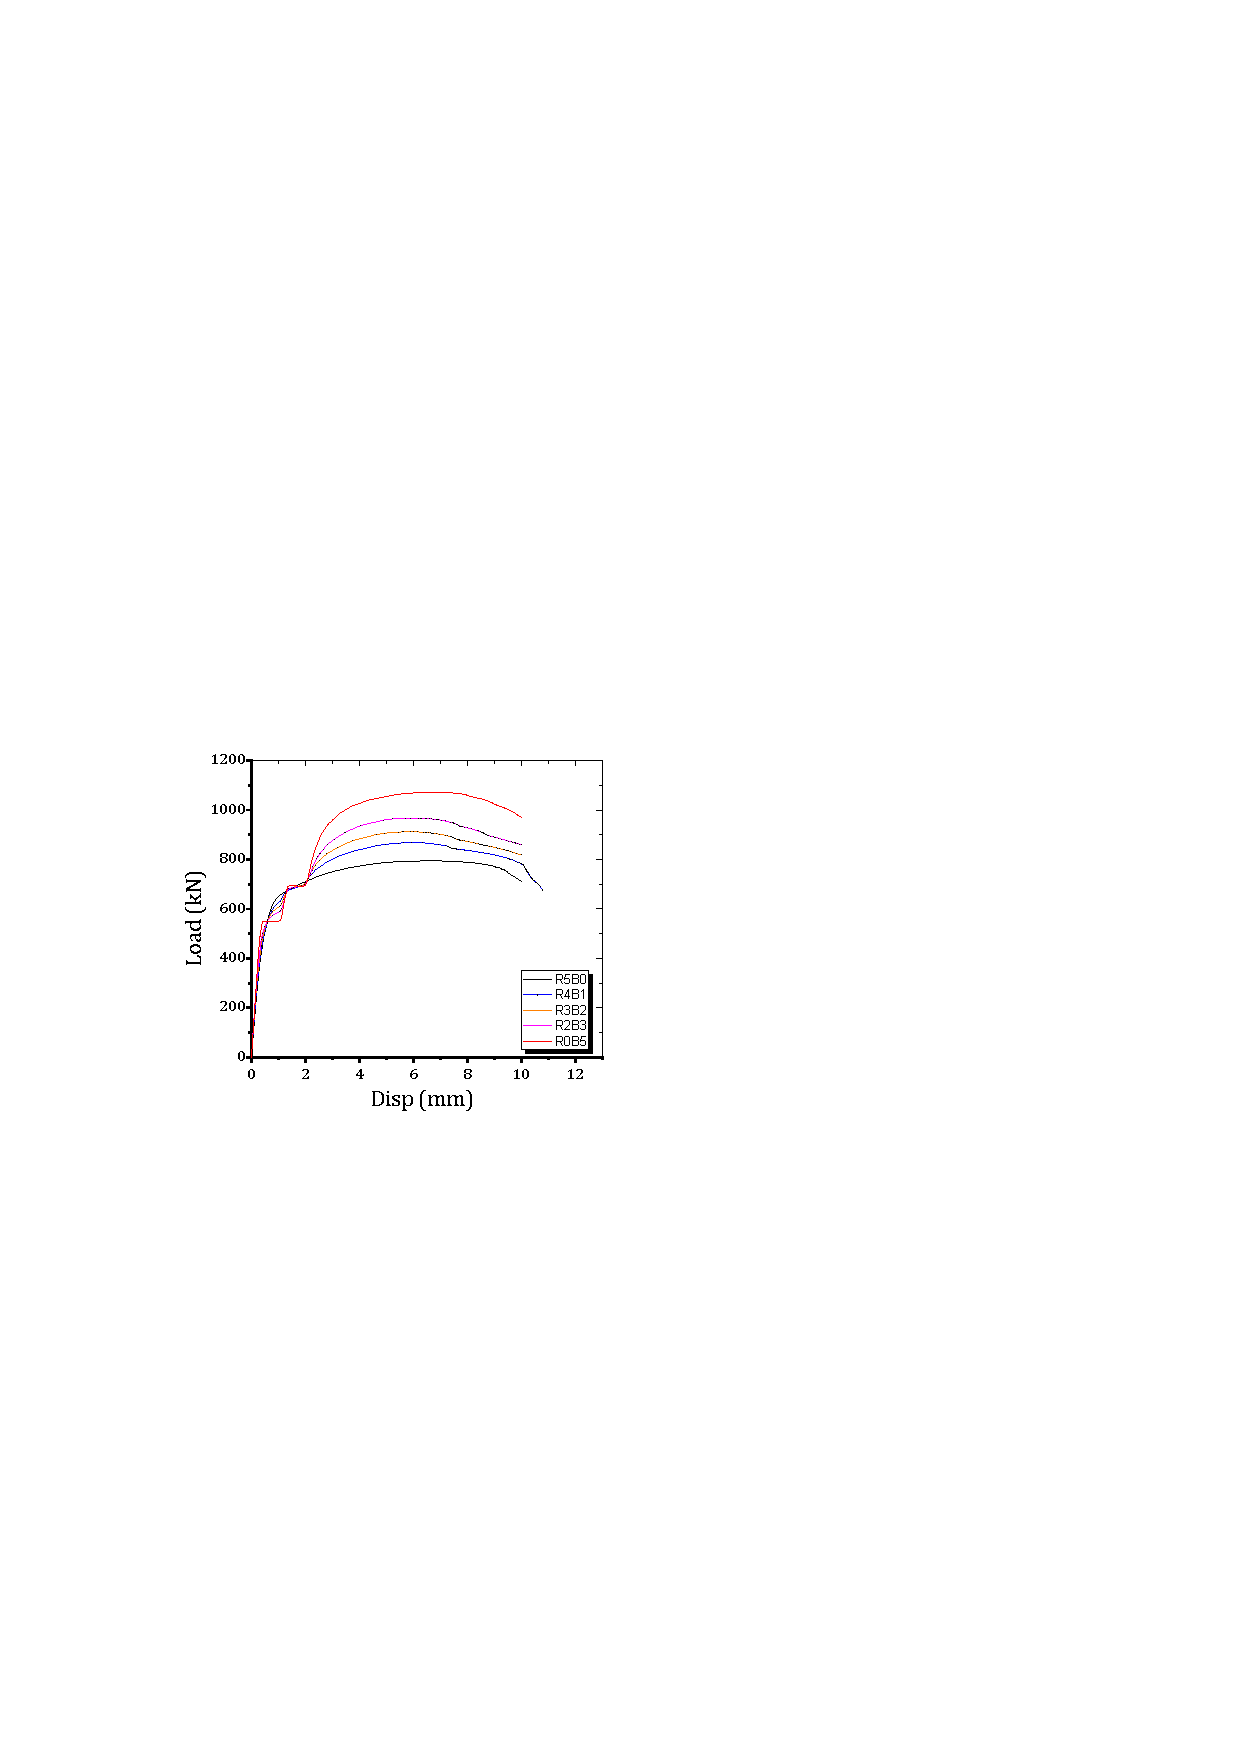
\includegraphics[width=0.7\linewidth]{imgs//ch4/fig-5rld.pdf}
    \caption{The relationship between load and displacement}
    \label{fig-5rld}
\end{figure}

\subsubsection{Stress contour}

Fig.\ref{fig-5rslscount} shows the mises stress contour plot when each case begins to exhibit nonlinear behavior. When the joint begins to exhibit nonlinear behavior, the area around the hole in the main plate develops a plastic zone, but it does not develop to the gross section of the plate. On the other hand, the shaft of each rivet develops a plastic zone at the shear position. It was found that the nonlinear behavior in each case depends on the shear yield of the rivets. It can be confirmed from the contour plots that when the nonlinear behavior begins, the high-strength bolt of the joint is not yet in a bearing state, and the stress around the hole in the main plate to the high-strength bolt is small. In the R0B5 case, there is no stress around the hole due to bearing pressure because of the occurrence of slip in the nonlinear behavior.

\begin{figure}
    \centering
    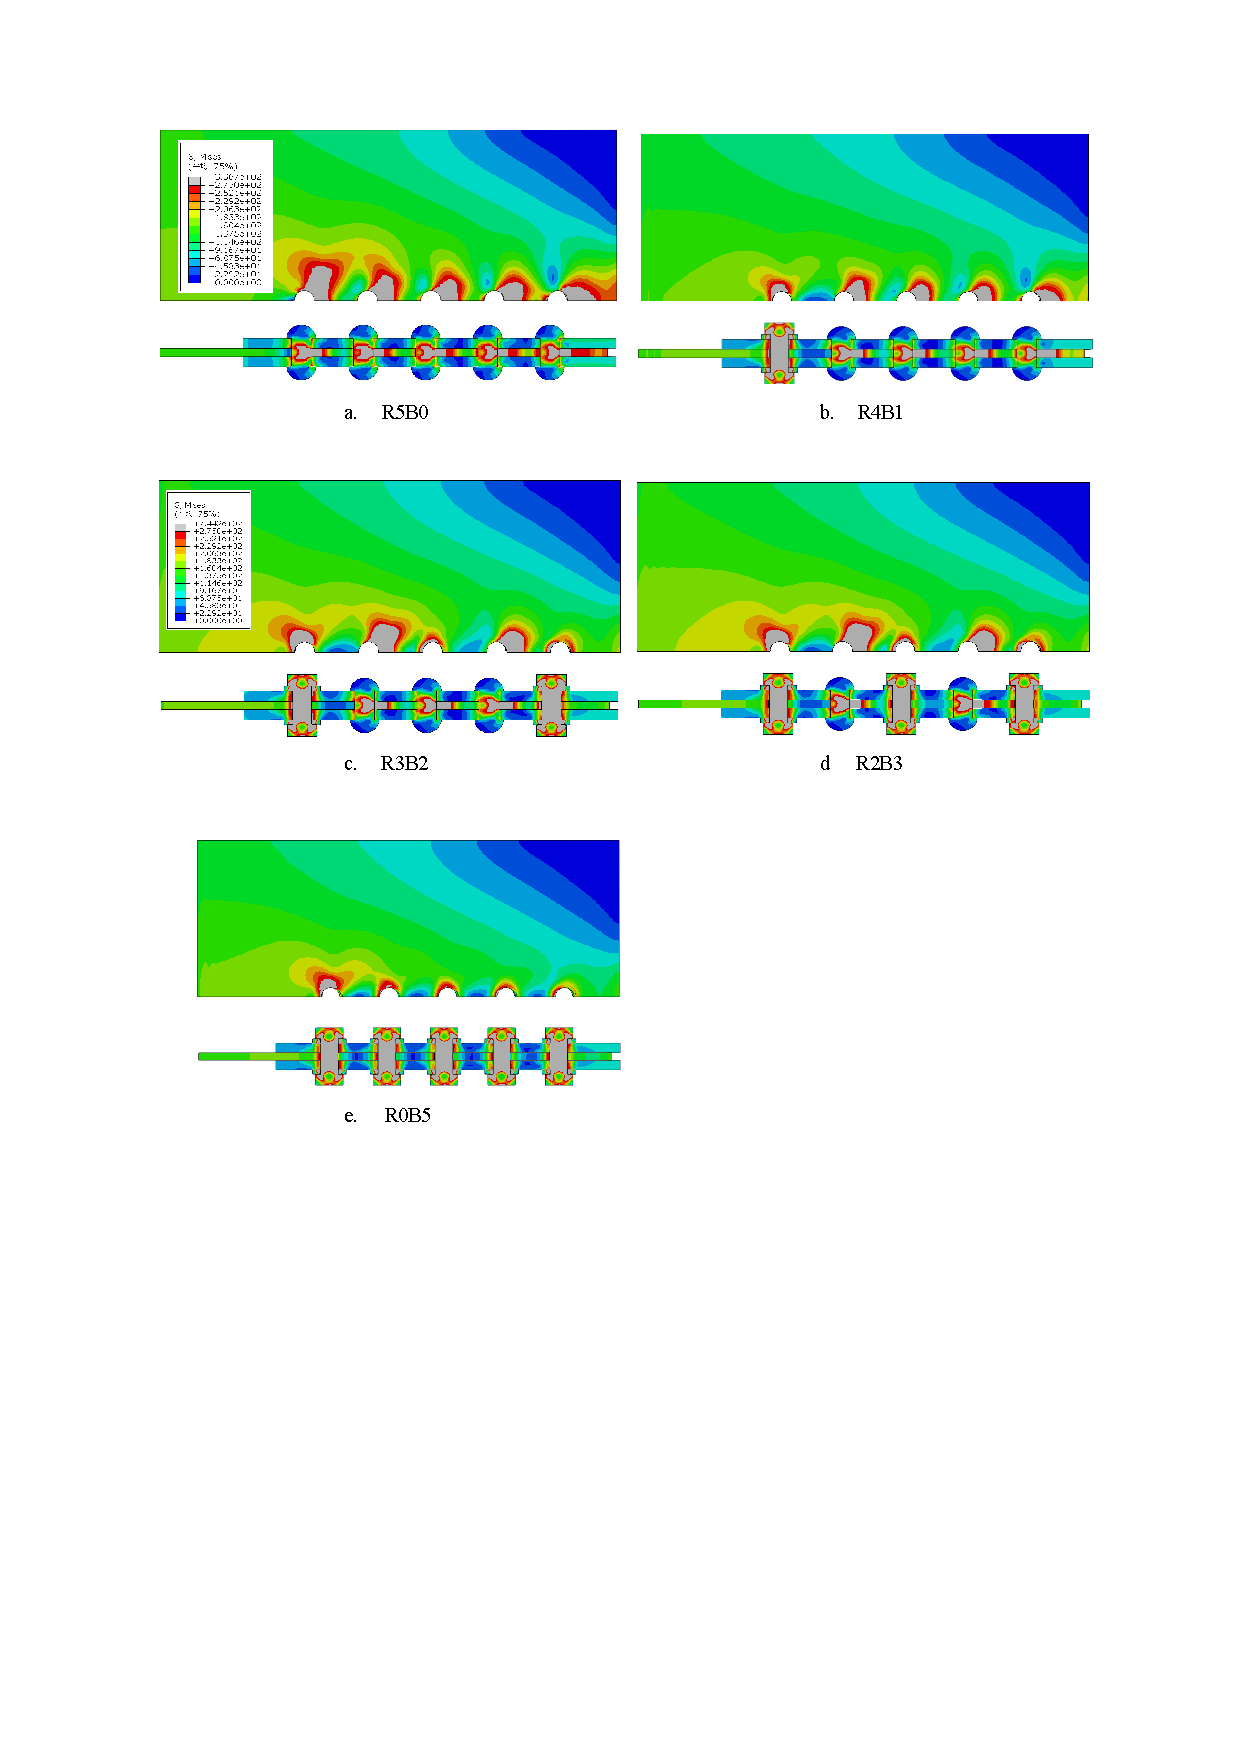
\includegraphics[width=1\linewidth]{imgs//ch4/fig-5rslscount.pdf}
    \caption{Mises stress contour plot when each case begins to exhibit nonlinear behavior}
    \label{fig-5rslscount}
\end{figure}

In the riveted joints, the plastic zone at the rivet axis is smaller than in other cases during linear behavior, but the stress in the welded material is relatively high. Especially at the edge, there is a clear tendency for the plastic zone to extend to the edge. Failure due to bearing of the joined material may occur at an early stage.


Fig.\ref{fig-5rulscount} shows the mises stress contour plot of each case when max load. It can be determined that the maximum load of the riveted and hybrid joint depends on the shear yield of the rivet. The rivet shaft is in the plastic zone and the tensile strength of the rivet is close to the rivet's ultimate strength $f_{ur}$ at the maximum load. The ultimate failure of the rivet is assumed to be the rivet shear rupture. On the other hand, in the high-strength bolt friction joint case, the shaft of the high-strength bolt did not yet develop a plastic zone, but developed a plastic zone around the hole in the main plate up to the gross section of the plate. In the high-strength bolt friction joint case, it can be inferred that the final failure is either net cross-sectional rupture or end shear failure of the main plate. 

The stress propagation in the plastic zone around the hole is different for each case, and the stress propagation is small from the outside to the inside of the joint. The direction of the plastic zone changes depending on the number of high-strength bolts replaced. In the case of rivet and single rivet replacement, the plastic zone tended to propagate toward the center of the plate width on the tensile side. In the case of R2B3, the plastic zone tended to propagate in the diagonal direction.

\begin{figure}
    \centering
    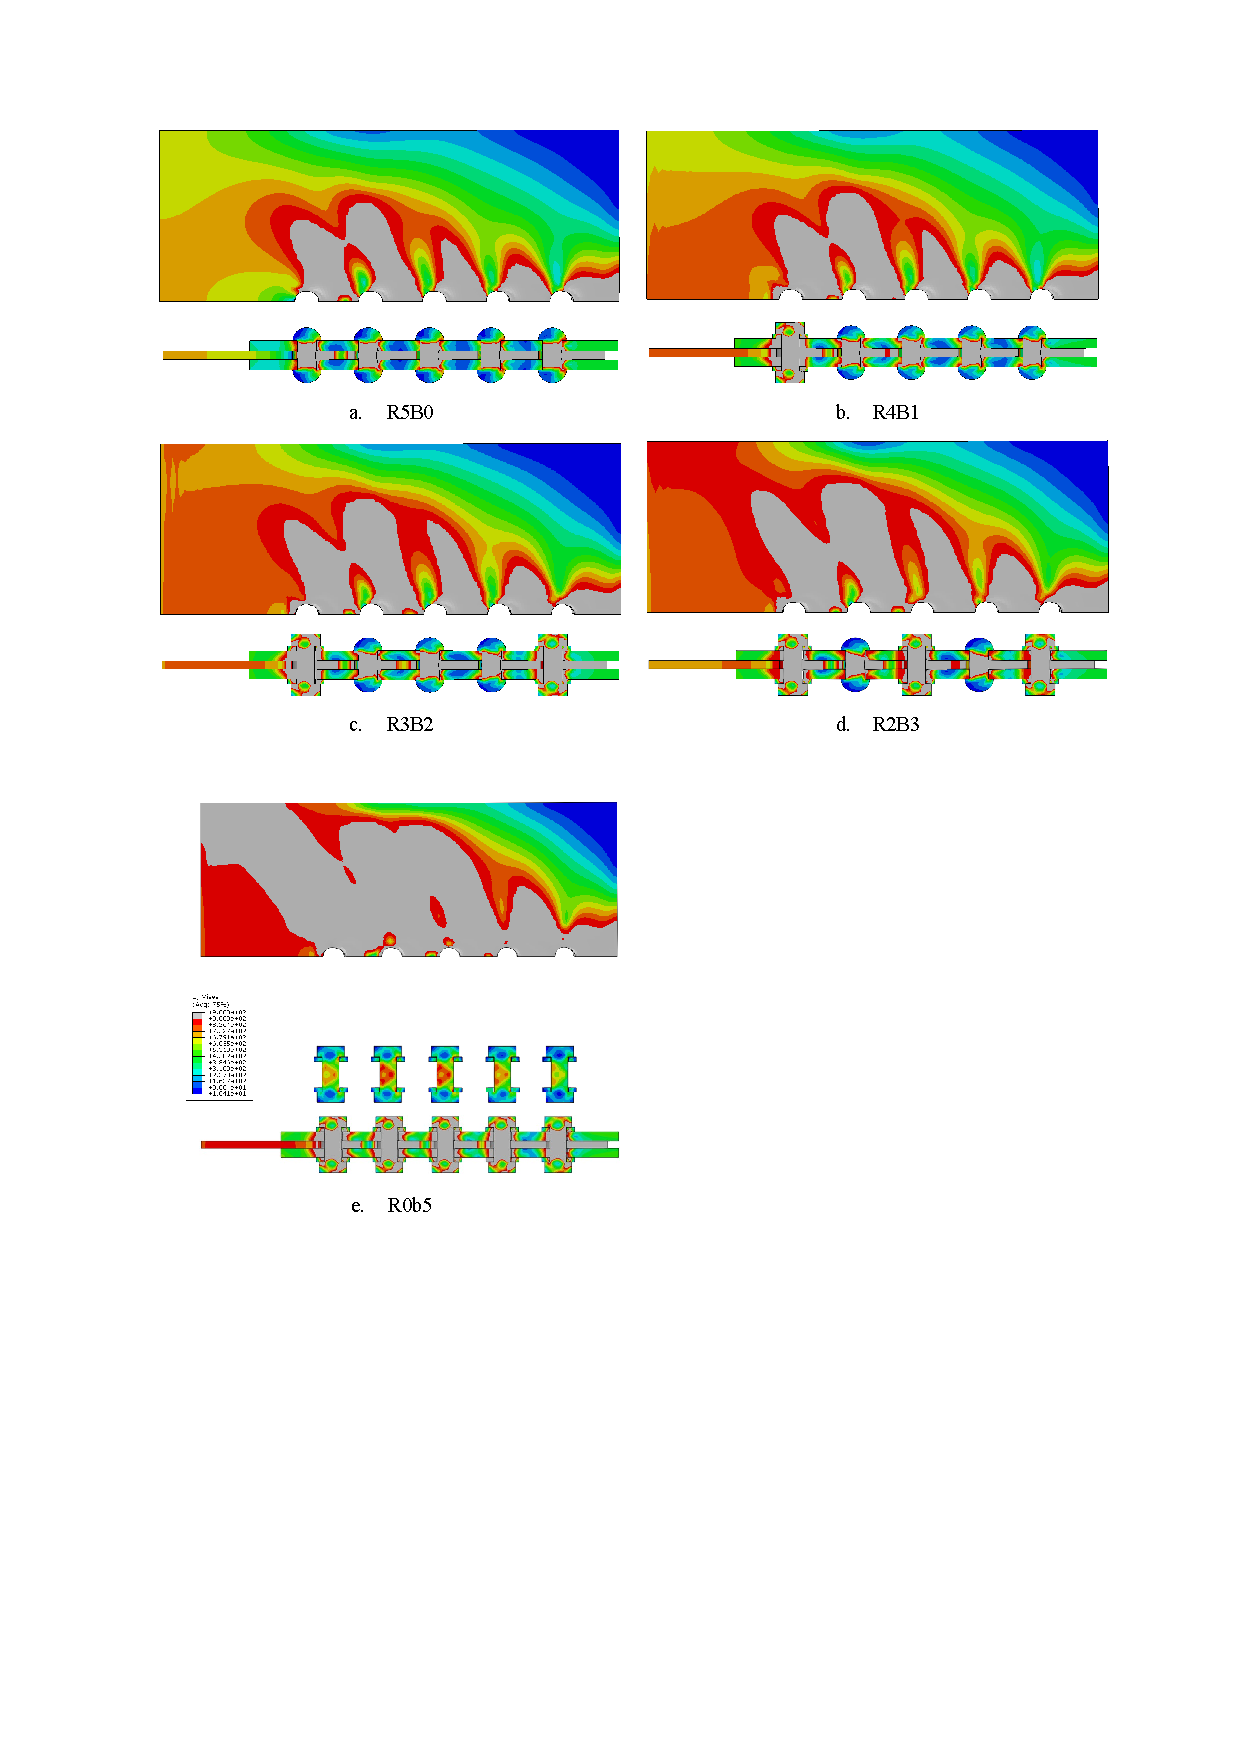
\includegraphics[width=1\linewidth]{imgs//ch4/fig-5rulscount.pdf}
    \caption{Mises stress contour plot of each case when max load}
    \label{fig-5rulscount}
\end{figure}

\subsubsection{Deformation of the hole}


Fig.\ref{fig-5rholedef} shows the deformation of each case each fastener's hole. The vertical axis is the hole deformation at each fastener hole, and the horizontal axis is the overall load. The bearing deformations of the riveted and high-strength bolt friction joints are almost equal. However, in the case of a hybrid joint, the changes in the deformations of the holes in the rivets and high-strength bolts are also different because the load-transfer mechanism is different. From Fig.\ref{fig-5rholedef} b, c, and d, the rate of change in the bearing deformation of the holes in the rivets is almost equal, and bearing deformation occurs at an earlier stage than that of the high-strength bolts. In all cases, when the average value reaches 5\%, the hole in the rivet has already exceeded 5\% of the deformation before that. Since the change in hole deformation is not uniform, the use of the average value to determine the limit state of the joint is a concern. The deformation of the hole in each rivet must be taken into account.

\begin{figure}
    \centering
    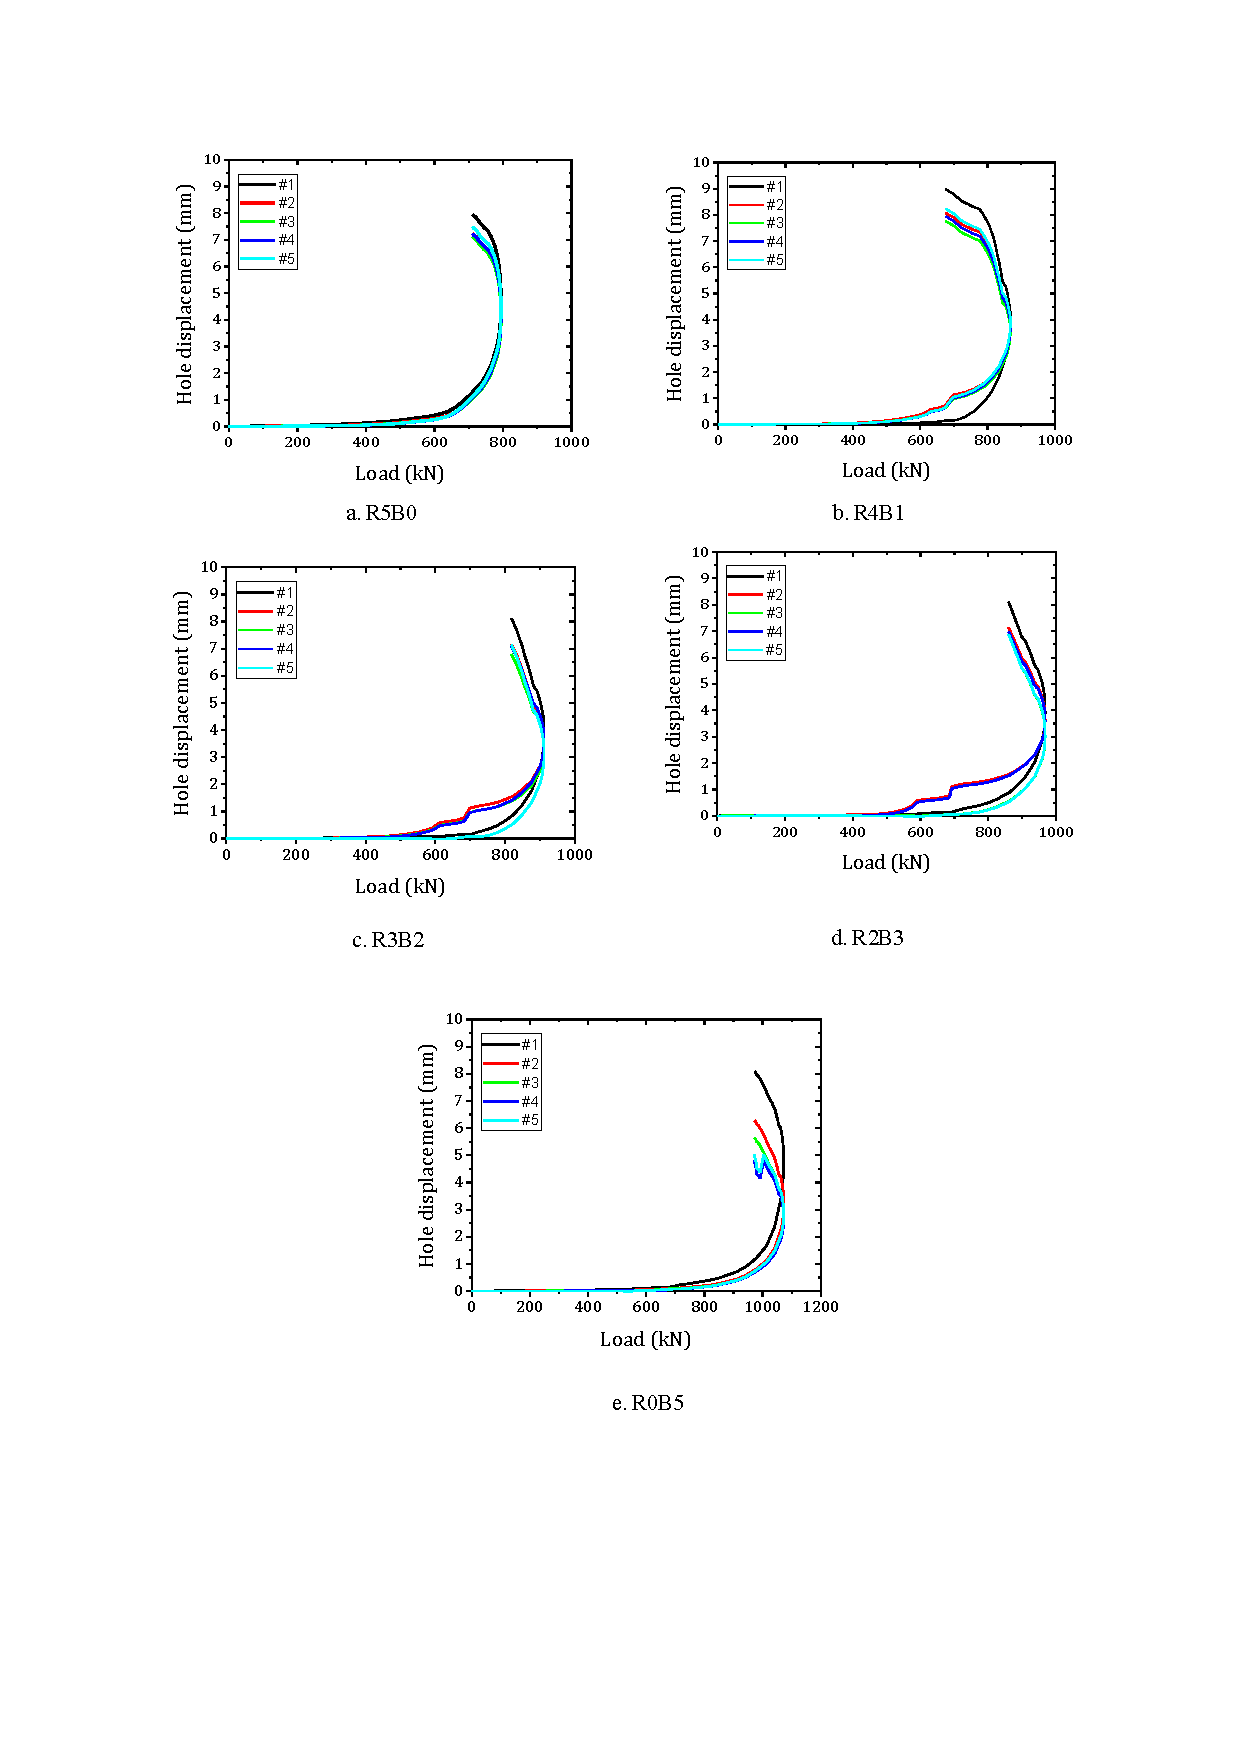
\includegraphics[width=1\linewidth]{imgs//ch4/fig-5rholedef.pdf}
    \caption{The deformation of each case each fastener's hole}
    \label{fig-5rholedef}
\end{figure}

\section{Conclusions}

In this chapter, a three-dimensional elasto-plastic finite displacement analysis was conducted using rivet and high-strength bolt arrangements as parameters to elucidate the load transfer mechanism of a joint using a riveted joint and a high-strength bolt friction joint, considering the preload introduced during tightening. In order to focus on the yielding around the rivet holes in the main plate due to the supporting pressure of the rivets, the plate width b was varied while the plate thickness t was kept constant.

In this chapter, the displacement of the joint, the load sharing of each fastener, and the stress properties of the main plate were used to clarify the load transfer mechanism of the combined riveted and high-strength bolted friction joints with preloads taken into account.

The findings of this chapter are as follows.

\begin{enumerate}
    \item In this study, we focused on the overall displacement of the joint and plastic deformation around the fastener hole, and defined the service limit state of the joint as the time when the load-overall displacement relationship begins to exhibit nonlinear behavior. It was found that the arrangement of the high-strength bolts had almost no effect on the service condition of the three-row joints.

    \item  In the case of the pressure-precedence type, where the critical service condition is determined by the bearing pressure, all rivet holes yielded when the load-total displacement relationship of the entire joint began to exhibit nonlinear behavior, and the load at that time was consistent with Equation (9), which is calculated as the sum of the sliding capacity and bearing pressure capacity of each fastener. In the case of the pure sectional yield-precedence type where the service limit state is determined by the net sectional yield, the net sectional yield is superior to the deformation due to bearing pressure, and the net sectional yield load can be evaluated using the net sectional yield capacity equation (7).

    \item  In a hybrid joint, the load is transferred by three processes: (1) a friction transfer phase in which the load is transferred almost exclusively by friction up to a slip capacity Fslip , (2) a combined transfer phase in which the load is transferred by bearing pressure and friction up to a bearing pressure load $P_{bya}$ , and (3) a plastic deformation phase in which the joint is plastically deformed afterwards. The combined joint not only increases the initial stiffness of the joint compared to a riveted joint, but also relieves the bearing stress on the rivet because the load is transmitted by the contact plate through friction.

    \item  In the pure-section yield-precedence case, the net sectional yield capacity of the case with fastener position 1 as a high-strength bolt increased approximately 10\% and the initial stiffness also increased compared to the fully riveted case because the load was transferred to the bracing plate by frictional force. In the case with high-strength bolts at fastener positions 2 and 3, the joint had higher initial stiffness than the fully riveted case, but the difference in net cross-sectional yield strength was smaller.

    \item In the case of the support-precedence type, the difference in the support load between the all-rivet case and the combined-joining case is small regardless of the bolt arrangement, but the combined-joining case is affected by frictional forces. (preload). HSB0 is not included in the comparison because the rivet preload could not be determined in the experiment.

\end{enumerate}

\textbf{Load redistribution when remove rivet}
 
When replace the rivet, the load sharing behavior will change, especially remove one rivet, the load will transfer to the other rivet, the transfer mechanism is important. An FE analysis was conducted to simulate the load redistribution when the rivet was removed under a dead load. Based on the results obtained, the following conclusions were inferred:

\begin{enumerate}
    \item When the end rivet (i.e., rivet \#1 or rivet \#5) was removed, one-half of the removed rivet load share was transferred to the rivet closest to the removed rivet, and less load was transferred to more distant rivets.

    \item When the rivet in the middle of the joint (e.g., rivet \#3) was removed, the load was redistributed more evenly over the individual rivets.

    \item When a rivet was replaced by a bolt, the load transfer in rivets closer to the bolt was affected more, whereas more distant rivets were almost unaffected.

    \item The effect of replacing rivets other than rivet \#1 on the overall mechanical behavior of the joint was insignificant. When rivet \#1 was replaced by a bolt, bolt \#1 transferred more load to the cover plate by friction, thereby relieving the net cross-section stress in the connected plate.
    
\end{enumerate}




